\documentclass[a4paper]{article}

\setlength{\parindent}{0pt}
\setlength{\parskip}{1em}

\pagestyle{headings}

\usepackage{amssymb}
\usepackage{amsmath}
\usepackage{amsthm}
\usepackage{mathtools}
\usepackage{graphicx}
\usepackage{hyperref}
\usepackage{color}
\usepackage{microtype}
\usepackage{tikz}
\usepackage{pgfplots}
\usepackage{pgfplotstable}

\newcommand{\N}{\mathbb{N}}
\newcommand{\Q}{\mathbb{Q}}
\newcommand{\Z}{\mathbb{Z}}
\newcommand{\R}{\mathbb{R}}
\newcommand{\C}{\mathbb{C}}
\newcommand{\D}{\mathcal{D}}
\renewcommand{\S}{\mathcal{S}}
\renewcommand{\P}{\mathbb{P}}
\newcommand{\F}{\mathbb{F}}
\newcommand{\E}{\mathbb{E}}
\newcommand{\bra}{\langle}
\newcommand{\ket}{\rangle}


\graphicspath{{Image/}}

\hypersetup{
    colorlinks=true,
    linktoc=all,
    linkcolor=blue
}

\theoremstyle{definition}
\newtheorem*{axiom}{Axiom}
\newtheorem*{claim}{Claim}
\newtheorem*{conv}{Convention}
\newtheorem*{coro}{Corollary}
\newtheorem*{defi}{Definition}
\newtheorem*{eg}{Example}
\newtheorem*{lemma}{Lemma}
\newtheorem*{notation}{Notation}
\newtheorem*{prob}{Problem}
\newtheorem*{post}{Postulate}
\newtheorem*{prop}{Proposition}
\newtheorem*{rem}{Remark}
\newtheorem*{thm}{Theorem}

\DeclareMathOperator{\vdiv}{div}
\DeclareMathOperator{\grad}{grad}
\DeclareMathOperator{\curl}{curl}
\DeclareMathOperator{\Ann}{Ann}
\DeclareMathOperator{\Fit}{Fit}
\DeclareMathOperator{\Diag}{Diag}
\DeclareMathOperator{\tr}{tr}
\DeclareMathOperator{\im}{im}
\DeclareMathOperator{\Mat}{Mat}
\DeclareMathOperator{\Log}{Log}
\DeclareMathOperator{\Isom}{Isom}
\DeclareMathOperator{\Mesh}{Mesh}
\DeclareMathOperator{\Sym}{Sym}
\DeclareMathOperator{\Aut}{Aut}
\DeclareMathOperator{\cosech}{cosech}
\DeclareMathOperator{\Card}{Card}
\DeclareMathOperator{\Gal}{Gal}


\begin{document}

\title{Electromagnetism}

\maketitle

\newpage

\tableofcontents

\newpage

\section{Introduction and Definitions}

\subsection{Electric charges and currents}

The \emph{charge} of a particle is an intrinsic property (like mass) determining the strength of the EM forces it experiences. Charge is \emph{quantized} (discrete), always being a multiple $m \in \Z$ of the electron charge $q=-e$, where
\begin{equation*}
\begin{aligned}
e= 1.60217662(1) \times 10^{-19} C
\end{aligned}
\end{equation*}
where $C$ is Coulomb (SI unit of charge).

Charge can be positive, negative or zero (natural). Examples: electrons ($q=-e$), positrons ($q=e$), proton ($q=e$), neutron ($q=0$).

The \emph{charge density} $\rho(x,t)$ describes charge per unit volume.

For a single particle $q$ at positron $x'$, we have
\begin{equation}\tag{1.1} \label{eq:1.1}
\begin{aligned}
\rho(x,t) = q \delta(x-x') 
\end{aligned}
\end{equation}

While for $N$ particles,
\begin{equation*}\tag{1.2} \label{eq:1.2}
\begin{aligned}
\rho(x,t) =\sum_{i=1}^N q_i \delta(x-xi)
\end{aligned}
\end{equation*}

where $q_i,x_i$ are charge and position for the $i^{th}$ particle, and $\delta$ satisfying
\begin{equation*}\tag{1.3} \label{eq:1.3}
\begin{aligned}
\delta(x-x')=0 \forall x \neq x'
\end{aligned}
\end{equation*}

\begin{equation*}\tag{1.4} \label{eq:1.4}
\begin{aligned}
\int_V \delta(x-x') d^3 x = \left\{\begin{array}{ll}
1 & x' \in V\\
0 & \text{ else}
\end{array}\right.
\end{aligned}
\end{equation*}
Also,
\begin{equation*}\tag{1.5} \label{eq:1.5}
\begin{aligned}
\int f(x) \delta(x-x') d^3 x = f(x')
\end{aligned}
\end{equation*}

We will also consider \emph{continuous} distributions $\rho(x,t)$ because $N$ is large (and in QM particles are described by continuous wave functions $\psi(x,t)$.

The \emph{total charge $Q$} in a volume $V$ is
\begin{equation*}\tag{1.6} \label{eq:1.6}
\begin{aligned}
Q = \int_V \rho(x,t) d^3 x
\end{aligned}
\end{equation*}

\emph{Electric current, $I$} describes the coherent motions of electric charge. We have
\begin{equation*}\tag{1.7} \label{eq:1.7}
\begin{aligned}
I = \frac{dQ}{dt}
\end{aligned}
\end{equation*}
across some surface $S$.

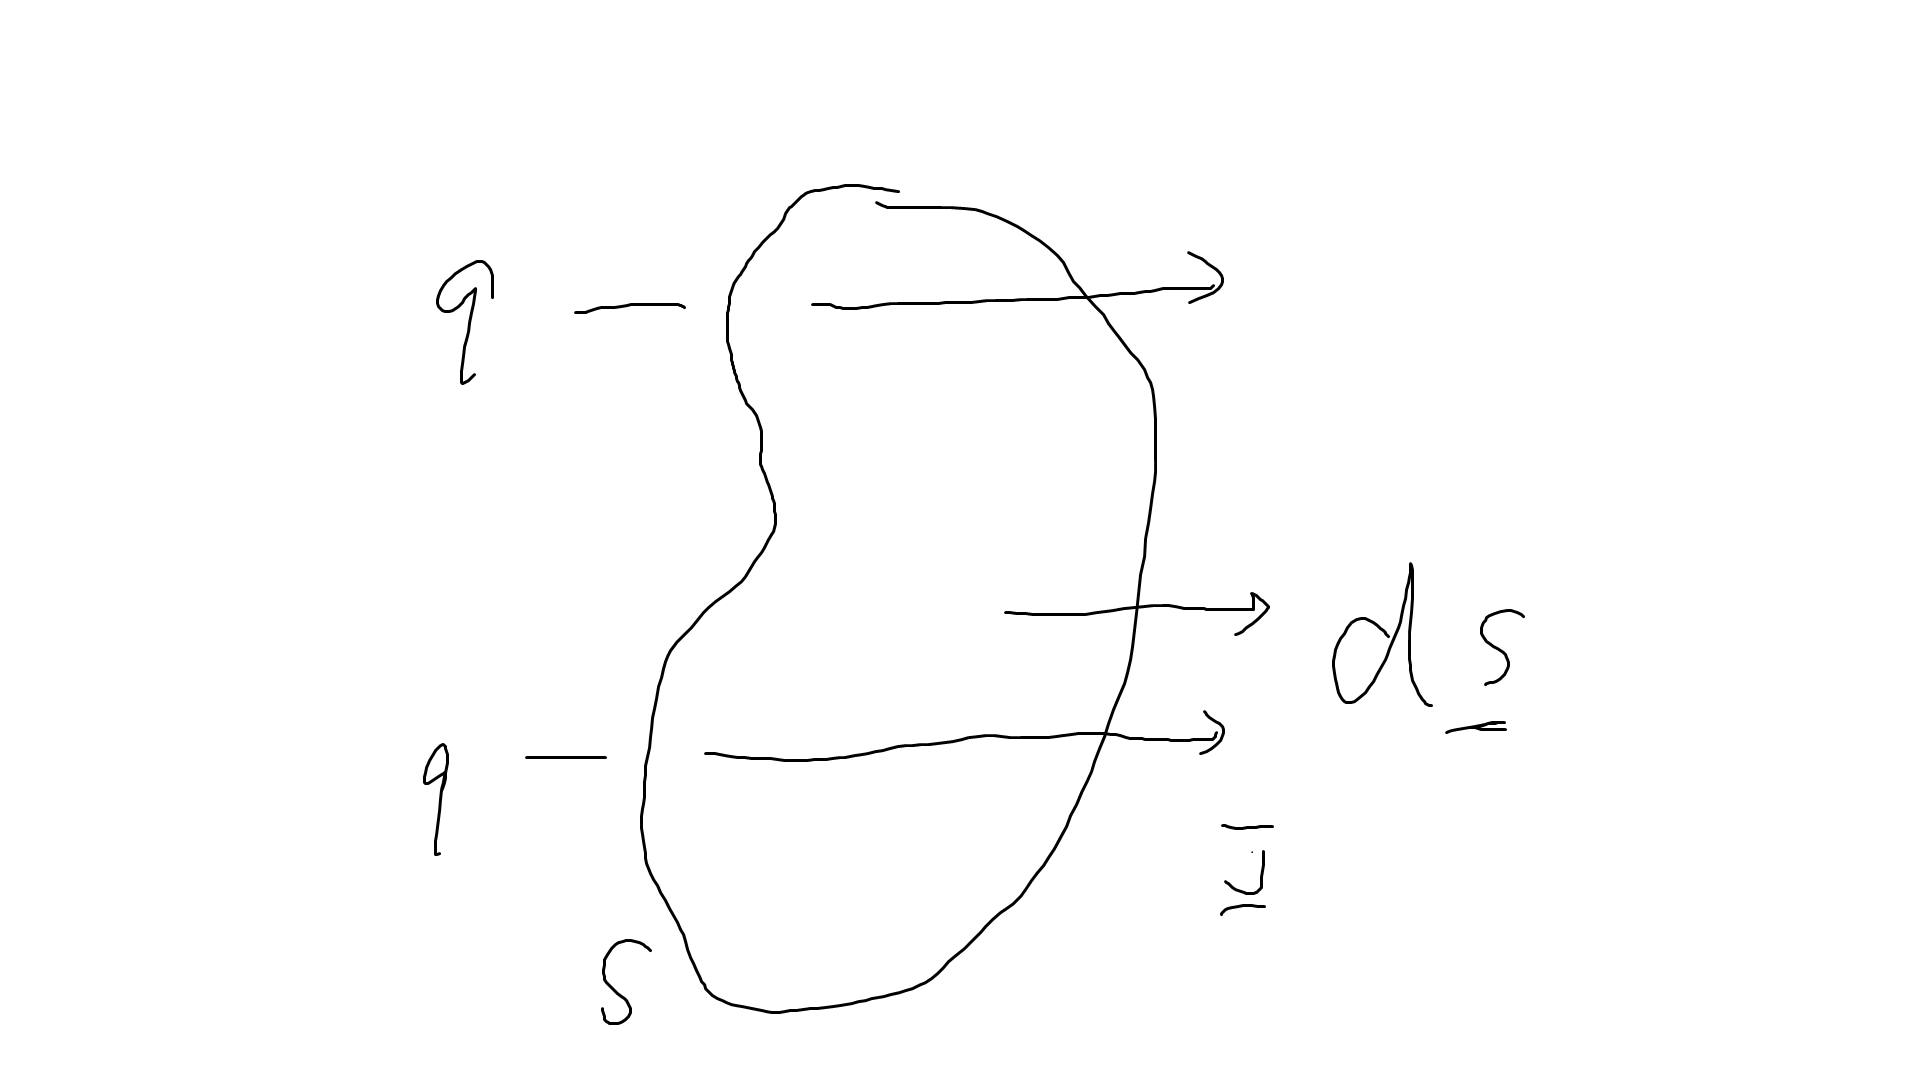
\includegraphics[scale=0.3]{EM_01}

Like fluid flow, we define a \emph{current density} $J(x,t)$, the rate charge passes across the surface element $d\mathbf{S} = \hat{\mathbf{m}} dS$ with normal $\hat{\mathbf{m}}$, that is, $dI = \mathbf{J} \cdot d\mathbf{S} = \mathbf{J} \cdot \hat{\mathbf{m}} dS$.

The total current across $S$ is then
\begin{equation*}\tag{1.8} \label{eq:1.8}
\begin{aligned}
I = \int_S \mathbf{J} \cdot d\mathbf{S}
\end{aligned}
\end{equation*}

Base SI unit of current is Ampere(A, $=Cs^{-1}$).

\begin{eg} Current in a wire.\\

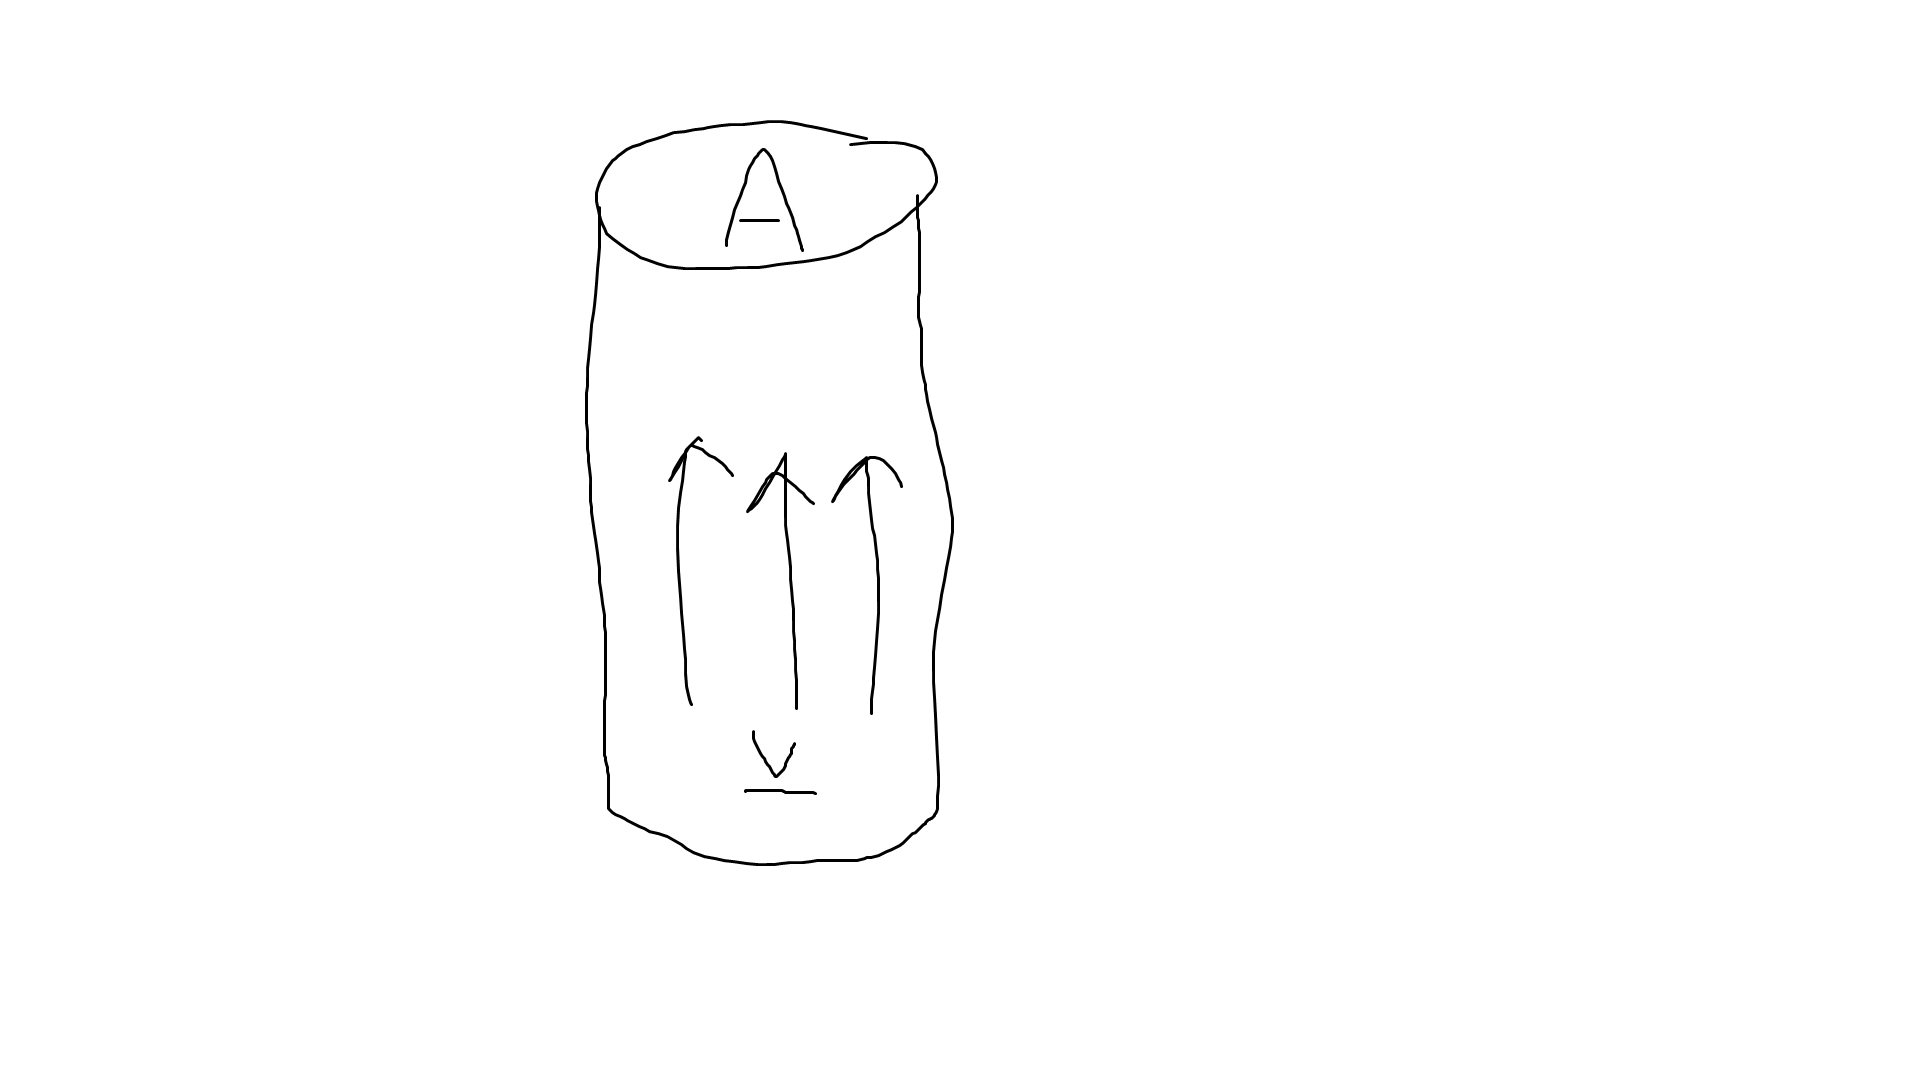
\includegraphics[scale=0.3]{EM_02}

Assume $1 A$ current in $1$mm diameter copper wire (lying in $z-$direction).\\
Uniform charge density: $\rho = ne$;\\
Electron density of Cu: $n=8 \times 10^{28} m^{-3}$;\\
Current density $\mathbf{J} = \rho \mathbf{v} = -env\mathbf{\hat{z}}$.

So the total current density is $d\mathbf{S} = \mathbf{\hat{z}}dS$. So
\begin{equation*}
\begin{aligned}
I&=\int_A \mathbf{J} \cdot d\mathbf{S}\\
&=-\int env\mathbf{\hat{z}}\cdot \mathbf{\hat{z}} dA\\
&=-env\pi R^2\\
&=-10^4 vCm^{-1}
\end{aligned}
\end{equation*}
But $I=1A$. So $v=10^{-4} ms^{-1}$.

\subsection{Forces and Fields}
The Lorentz force
\begin{equation*}\tag{1.9} \label{eq:1.9}
\begin{aligned}
\mathbf{F} = q(\mathbf{E} + \mathbf{v} \times \mathbf{B})
\end{aligned}
\end{equation*}
describes how a particle of charge $\mathbf{q}$ moves under the influence of an electric field $E(\mathbf{x},t)$ and a magnetic field $\mathbf{B}(\mathbf{x},t)$. SI unit for $\mathbf{E}$ are force per unit charge ($NC^{-1} = kgms^{-2}C^{-1}$).

The ratio $[E/B] = [V]$ means units for $B$, Tesla, are linked to particle motion (or currents in a wire) ($T=NC^{-1}m^{-1} s = N/(Am) = N/(Cms^{-1}) = 10^4 Gauss$).

Conversely, particles create EM fields, e.g. a static charge $Q$ at $\mathbf{r} = 0$ has
\begin{equation*}\tag{1.10} \label{eq:1.10}
\begin{aligned}
E(\mathbf{r}) = \frac{1}{4\pi\varepsilon_0} \frac{Q}{r^2} \mathbf{\hat{r}}
\end{aligned}
\end{equation*}
where the electric constant $\varepsilon_0 = 8.83 \times 10^{-11} C^2 kg^{-1} m^{-3}s^{-2}$ ($C^2N^{-1}m^{-2}$). Also note $\varepsilon_0 = \frac{1}{\mu_0 c^2}$ ($c$ is the speed of light) derives from the magnetic constant, where
\begin{equation*}
\begin{aligned}
\mu_0 &= 4\pi \times 10^{-7} C^{-2}kgm\\
&\approx 125 \times 10^{-6} C^{-2} kgm.
\end{aligned}
\end{equation*}

\end{eg}

Charge conservation is observed in every physical process. Charge $Q$ in a volume $V$ can only change by moving across a \emph{closed surface} $S$, i.e.
\begin{equation*}\tag{*}
\begin{aligned}
\int_S \mathbf{J} \cdot d\mathbf{S} &= \int_V \nabla \cdot \mathbf{J} dx^3\\
&= -\frac{dQ}{dt}
\end{aligned}
\end{equation*}
The negative sign is because outward normals imply current flows \emph{out} of $V$.

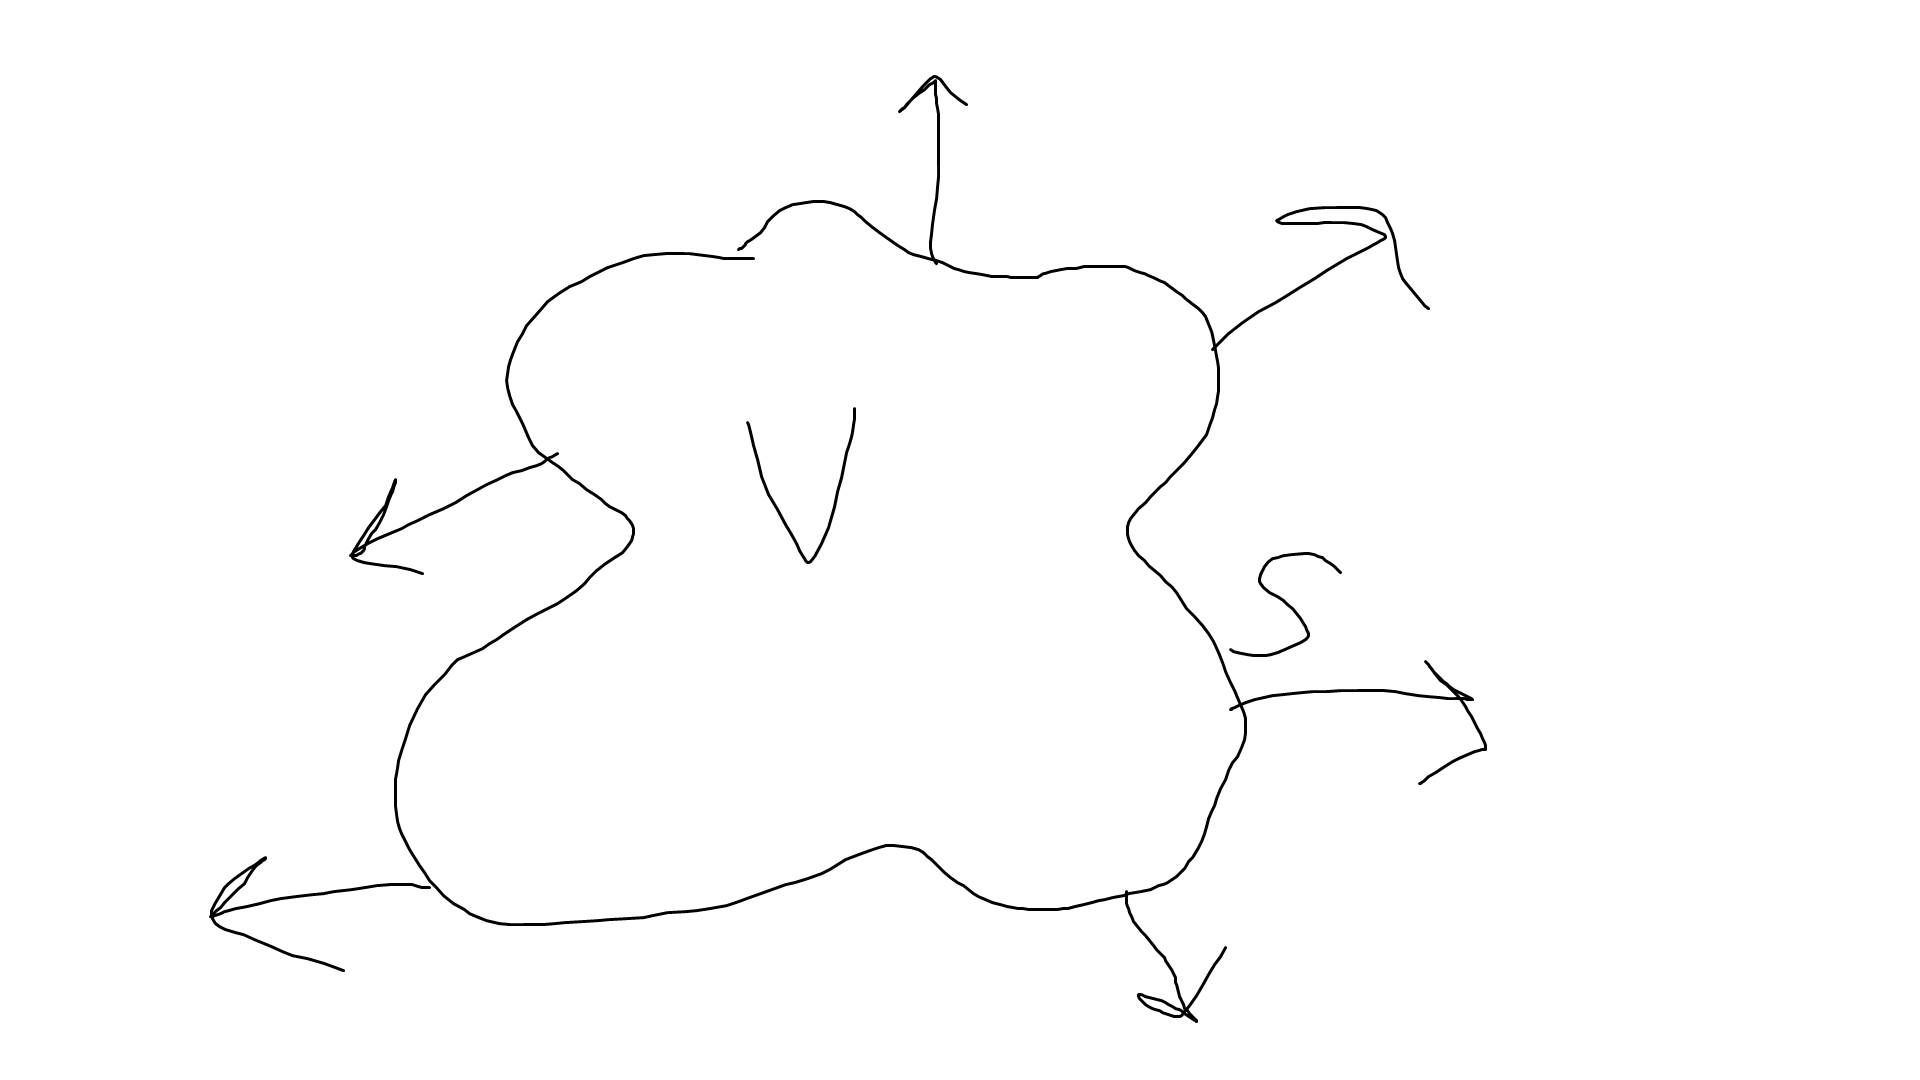
\includegraphics[scale=0.3]{EM_03}

But from definition \ref{eq:1.6},
\begin{equation*}\tag{$\dagger$}
\begin{aligned}
\frac{dQ}{dt} = \frac{d}{dt}\int_V \rho d^3 x = \int_v \frac{\partial \rho}{\partial t} d^3 x
\end{aligned}
\end{equation*}

So for arbitrary $V$, equation (*) and ($\dagger$) must imply a local conservation law
\begin{equation*}\tag{1.11} \label{eq:1.11}
\begin{aligned}
\frac{\partial \rho}{\partial t} + \nabla \cdot \mathbf{J} = 0
\end{aligned}
\end{equation*}

\subsection{Maxwell's equations}
All knowledge about the interplay between EM fields and particles is encoded in Maxwell's equations:
\begin{equation*}\tag{Gauss' Law, 1.12} \label{eq:1.12}
\begin{aligned}
\nabla \cdot \mathbf{E} = \frac{\rho}{\varepsilon_0}
\end{aligned}
\end{equation*}
\begin{equation*}\tag{Gauss' Law for magnetism, 1.13} \label{eq:1.13}
\begin{aligned}
\nabla \cdot \mathbf{B} = 0
\end{aligned}
\end{equation*}
\begin{equation*}\tag{Faraday's law of induction, 1.14} \label{eq:1.14}
\begin{aligned}
\nabla \times \mathbf{E} = -\frac{\partial \mathbf{B}}{\partial t}
\end{aligned}
\end{equation*}
\begin{equation*}\tag{Ampere-Maxwell Law, 1.15} \label{eq:1.15}
\begin{aligned}
\nabla \times \mathbf{B} = \mu_0 \mathbf{J} + \frac{1}{c^2} \frac{\partial \mathbf{E}}{\partial t}
\end{aligned}
\end{equation*}

\newpage

\section{Electrostatics}

Consider time-independent charge distribution $\rho(\mathbf{x},t)$ with $\mathbf{J}=0$ (allowing us to set $\mathbf{B} = 0$ in equation \eqref{eq:1.13} - \eqref{eq:1.15}). Given $\rho$, we seek solutions of
\begin{equation*}\tag{2.1} \label{eq:2.1}
\begin{aligned}
\nabla \cdot \mathbf{E} = \frac{\rho}{\varepsilon_0}
\end{aligned}
\end{equation*}
and
\begin{equation*}\tag{2.2} \label{eq:2.2}
\begin{aligned}
\nabla \times \mathbf{E} = 0.
\end{aligned}
\end{equation*}

\subsection{Gauss' Laws}
Integrate \eqref{eq:2.1} over a volume $V$ in $\R^3$ bounded by surface $S$:
\begin{equation*}
\begin{aligned}
\int_V \nabla \cdot \mathbf{E} d^3 x &= \int_S \mathbf{E} \cdot d\mathbf{S}\\
&= \frac{1}{\varepsilon_0} \int_V \rho d^3 x\\
&= \frac{Q}{\varepsilon_0}
\end{aligned}
\end{equation*}
by divergence theorem, \eqref{eq:2.1} and \eqref{eq:1.6} respectively.

This implies Gauss' Laws
\begin{equation*}\tag{2.3} \label{eq:2.3}
\begin{aligned}
\Phi_{flux} = \int_S \mathbf{E}\cdot d\mathbf{S} = \frac{Q}{\varepsilon_0}
\end{aligned}
\end{equation*}
where the middle is flux through $S$ and the right is total charge in $V$.

For example, in the diagram below, we have $\Phi_S = \Phi_{S'}$ since they both enclose the charge.

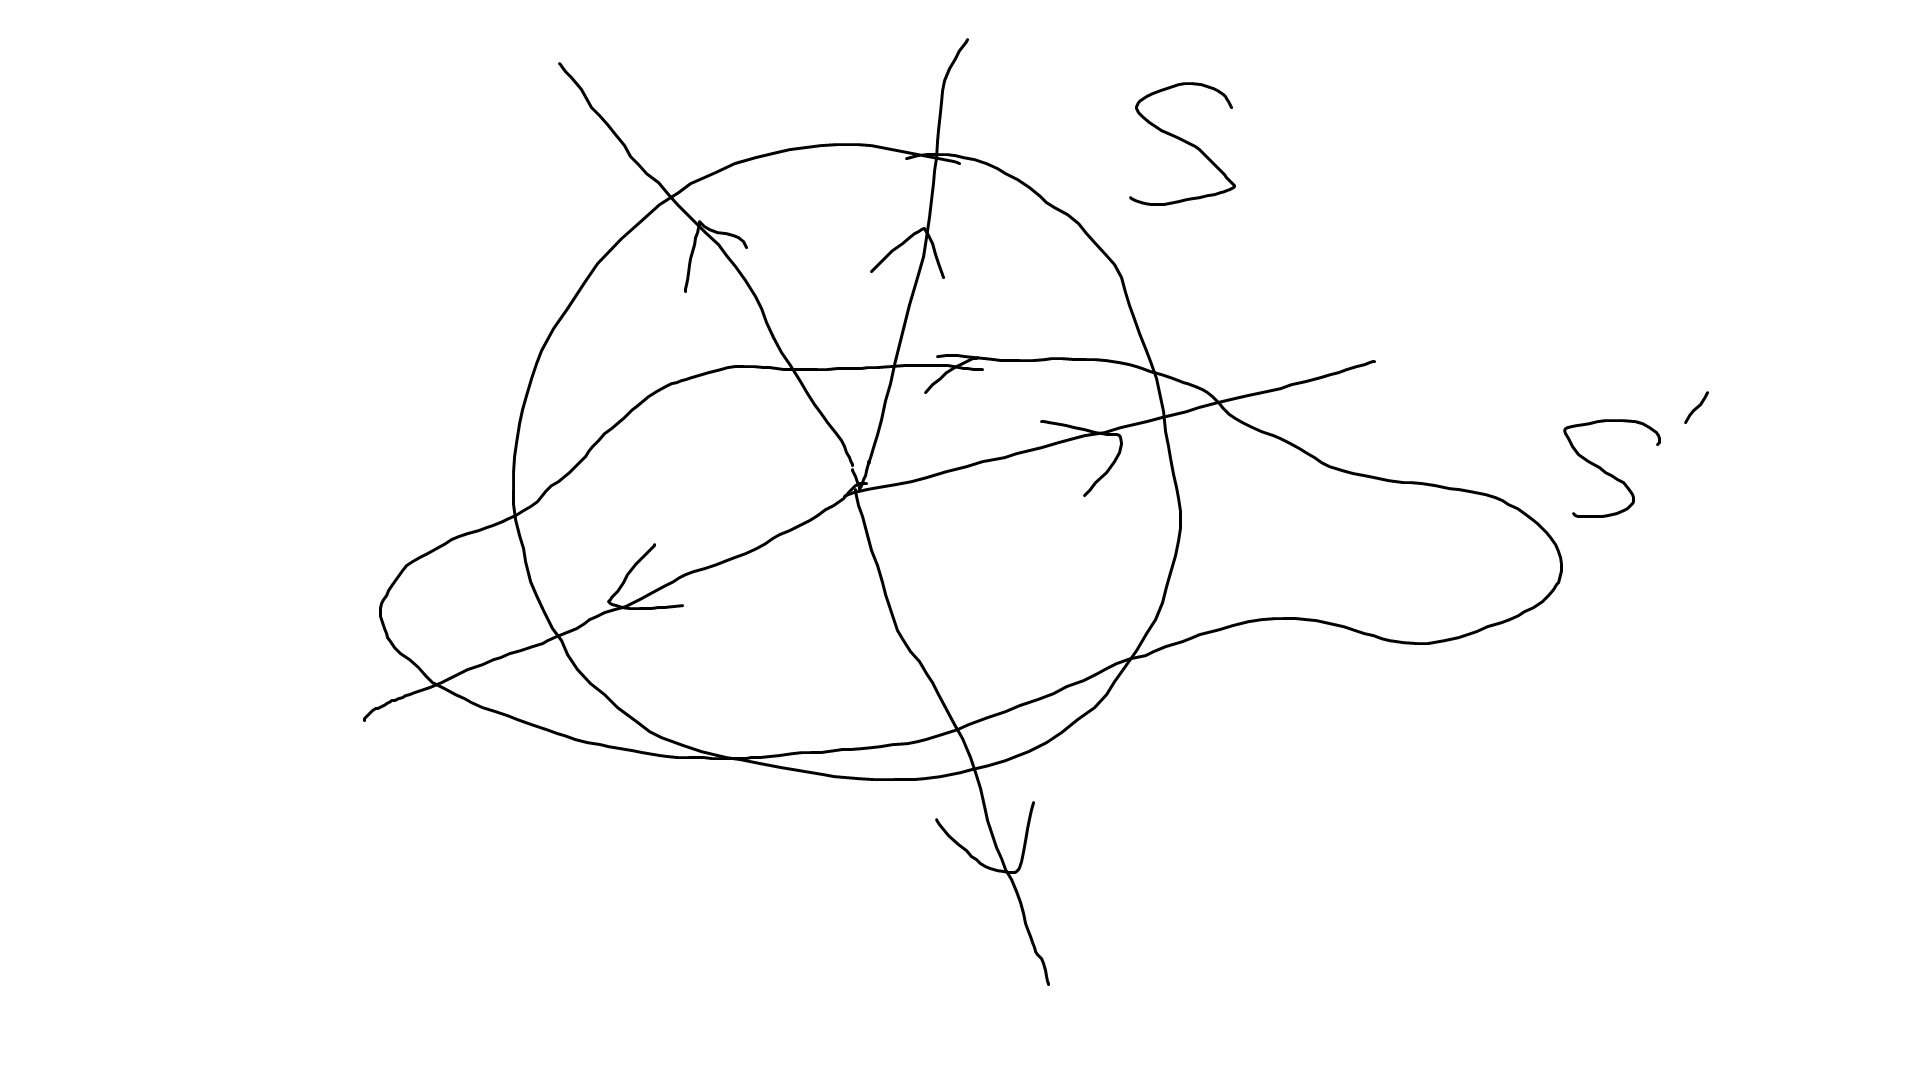
\includegraphics[scale=0.2]{EM_04}

While in the diagram below $\Phi_{S''} = 0$ since the total charge in $V$ is $0$.

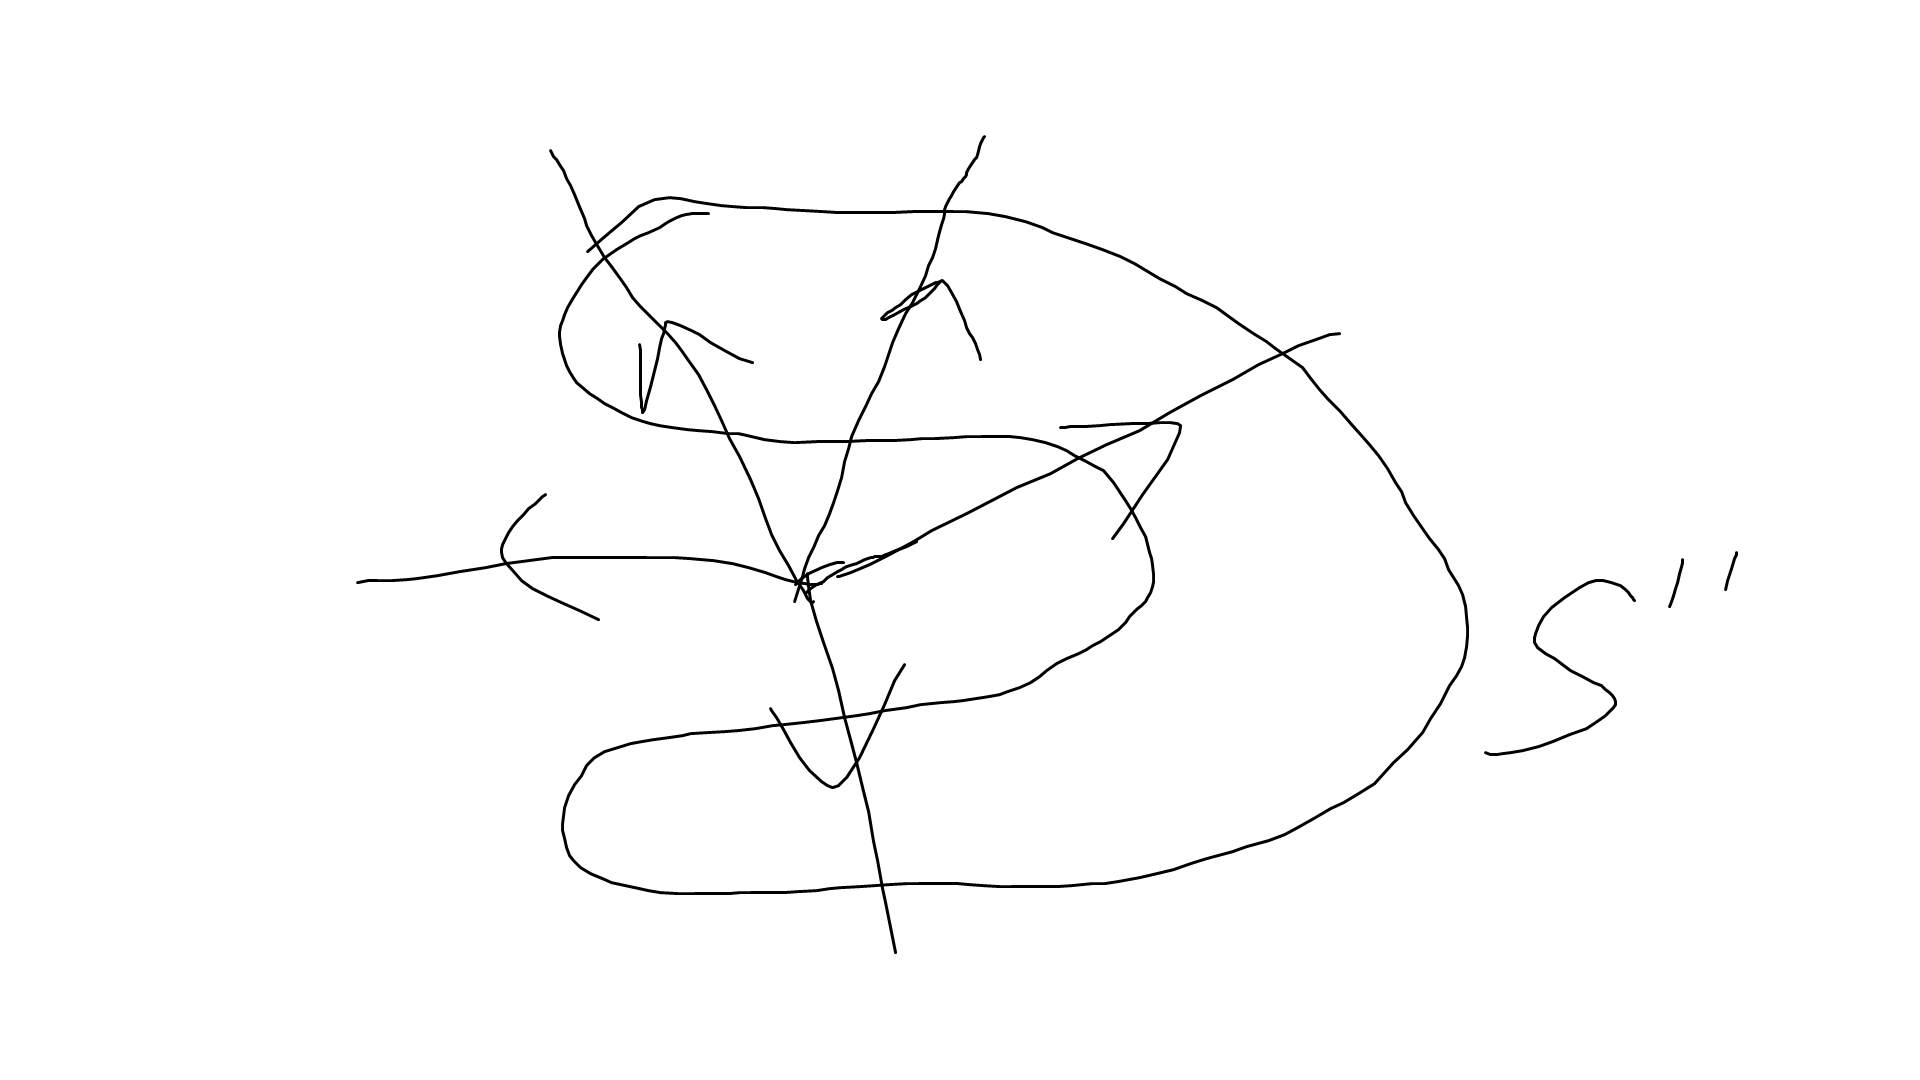
\includegraphics[scale=0.2]{EM_05}

Gauss' Law can be used to find solutions for $\mathbf{E}$ in situations of spherical symmetry.

\subsubsection{Application: Coulomb's Laws}

Suppose we have spherically symmetric charge distribution $\rho(\mathbf{r}) = \rho(r)$ with $r=|\mathbf{r}|$, $\rho(r) = 0$ for $r>R$.

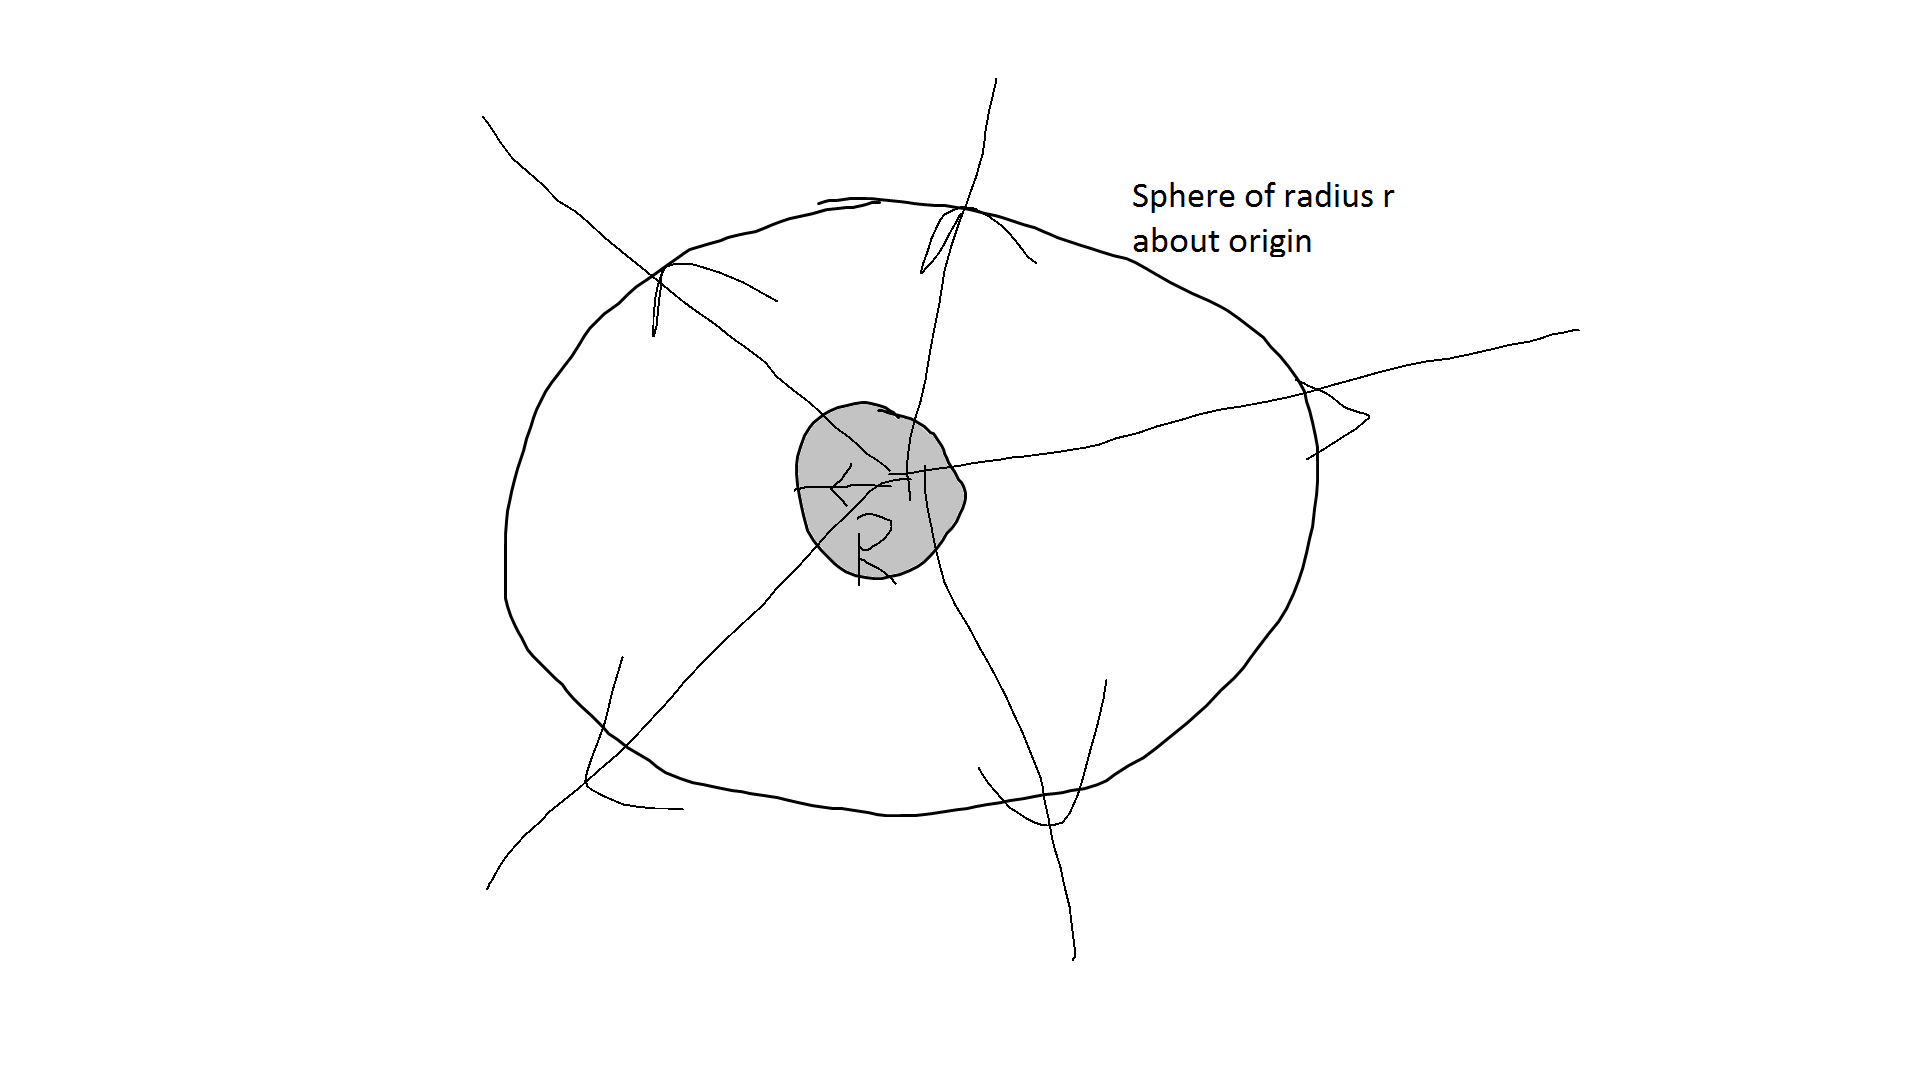
\includegraphics[scale=0.5]{EM_06}

Here,
\begin{equation*}
\begin{aligned}
\int_0^R \rho 4\pi r^2 dr = Q
\end{aligned}
\end{equation*}

By symmetry, $\mathbf{E} = E(r) \mathbf{\hat{r}}$ (so $\nabla \times \mathbf{E} = 0$). Gauss Law yields
\begin{equation*}
\begin{aligned}
\int_S \mathbf{E} \cdot d\mathbf{S} &= \int_S E(r)\mathbf{\hat{r}}\cdot d\mathbf{S}\\
&=E(r)4\pi r^2\\
&=\frac{Q}{\varepsilon_0}
\end{aligned}
\end{equation*}
(Note $d\mathbf{S} = r^2 \sin\theta d\theta d\phi \mathbf{\hat{r}}$).

This implies Coulomb's Law \eqref{eq:1.10},
\begin{equation*}\tag{2.4} \label{eq:2.4}
\begin{aligned}
\mathbf{E}(\mathbf{r}) = \frac{1}{4\pi \varepsilon_0} \frac{Q}{r^2} \mathbf{\hat{r}}, \ r>R
\end{aligned}
\end{equation*}

\textbf{Interior solution($r<R$)}: Suppose uniform distribution in sphere, i.e.
\begin{equation*}
\begin{aligned}
\rho(r) = \left\{\begin{array}{ll}
\rho_0 & r \leq R\\
0 & r>R
\end{array}\right.
\end{aligned}
\end{equation*}
where $\rho_0$ is some constant. Then the total charge is
\begin{equation*}\tag{*}
\begin{aligned}
Q = \frac{4\pi}{3} R^3 \rho_0
\end{aligned}
\end{equation*}
So
\begin{equation*}
\begin{aligned}
\int_S \mathbf{E} \cdot d\mathbf{S} &= E(r)4\pi r^2\\
&= \int_0^r \frac{\rho_0}{\varepsilon_0} 4\pi r^2 dr\\
&= \frac{1}{\varepsilon_0} \frac{4\pi}{3} r^3 \rho_0\\
&= \frac{Q}{\varepsilon_0} (\frac{r^3}{R^3})
\end{aligned}
\end{equation*}
using (*). So
\begin{equation*}\tag{2.5} \label{eq:2.5}
\begin{aligned}
\mathbf{E}(\mathbf{r}) = \frac{1}{4\pi \varepsilon_0} \frac{Qr}{R^3}\mathbf{\hat{r}} \ (r<R)
\end{aligned}
\end{equation*}

So the solution $\mathbf{E}$ looks like

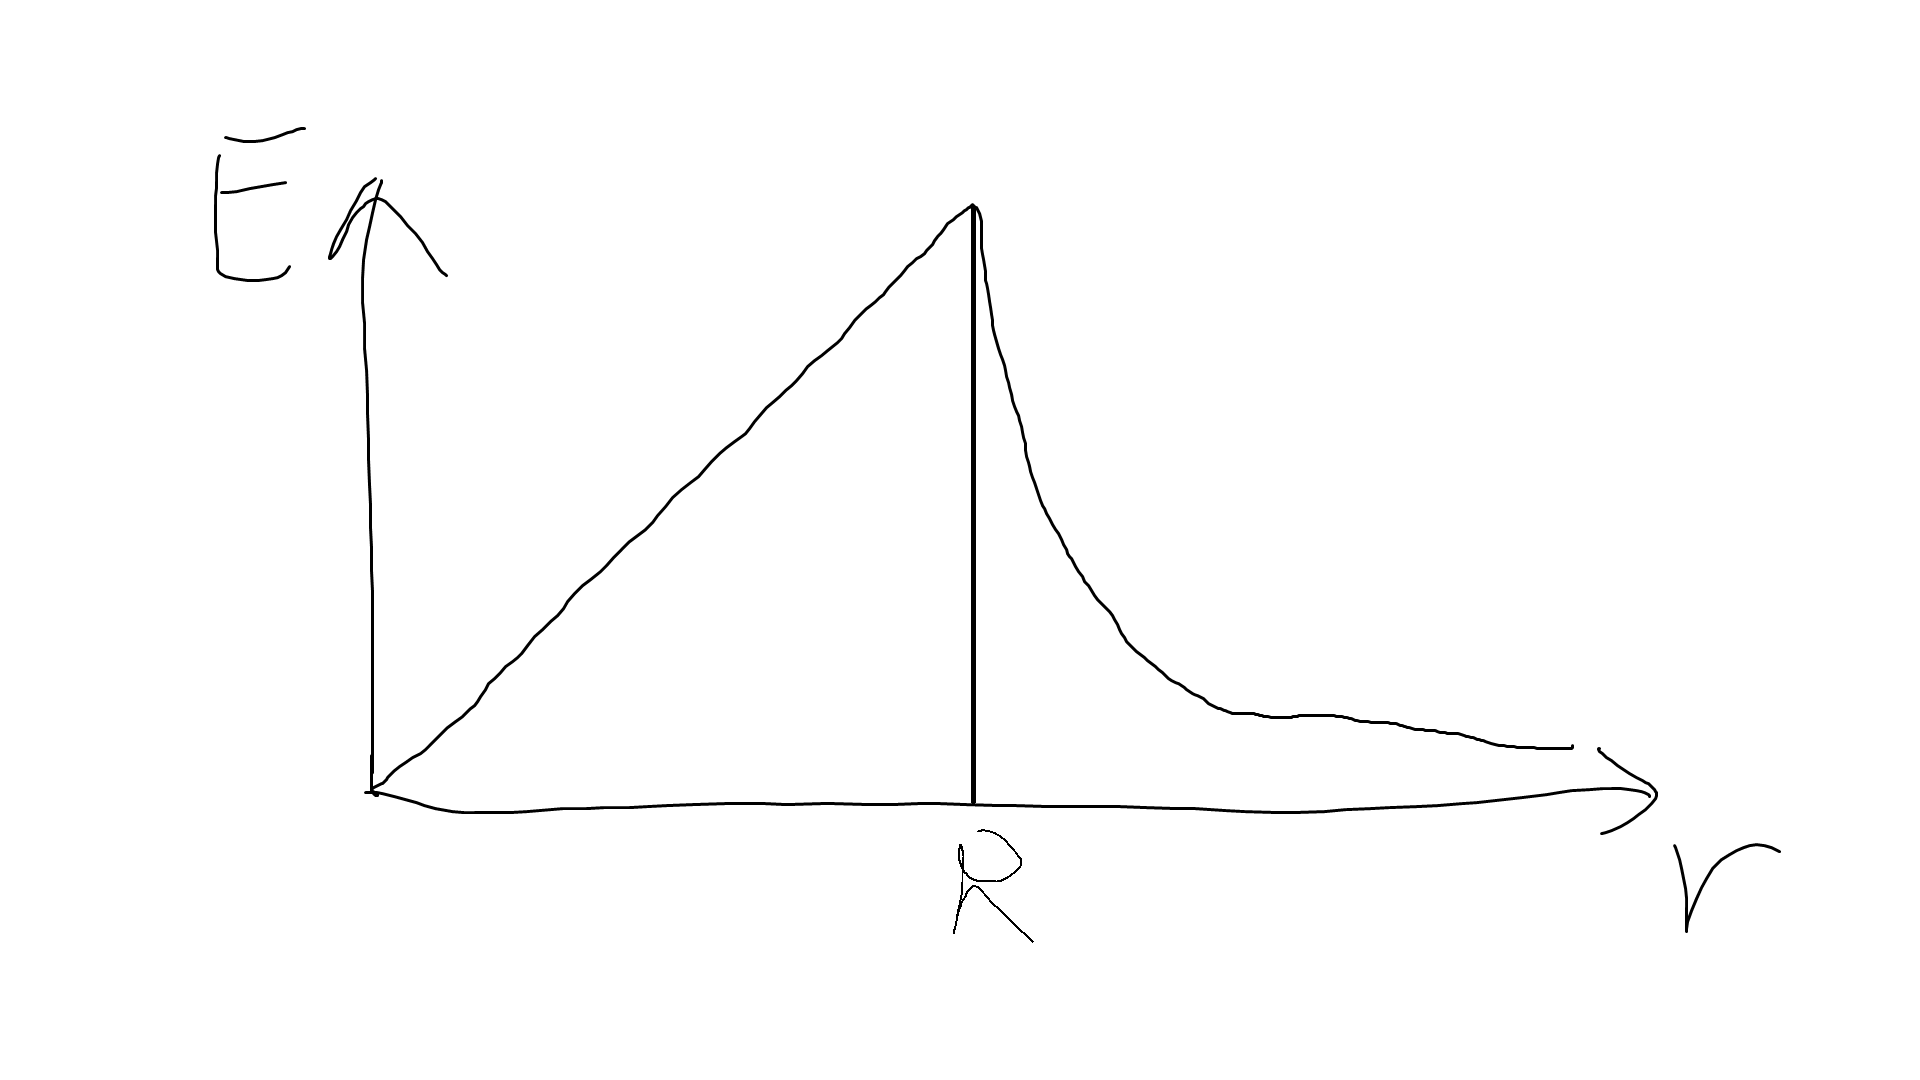
\includegraphics[scale=0.3]{EM_07}

\begin{eg} (Charged Line)\\
Consider a wire with constant charge $\eta$ per unit length.

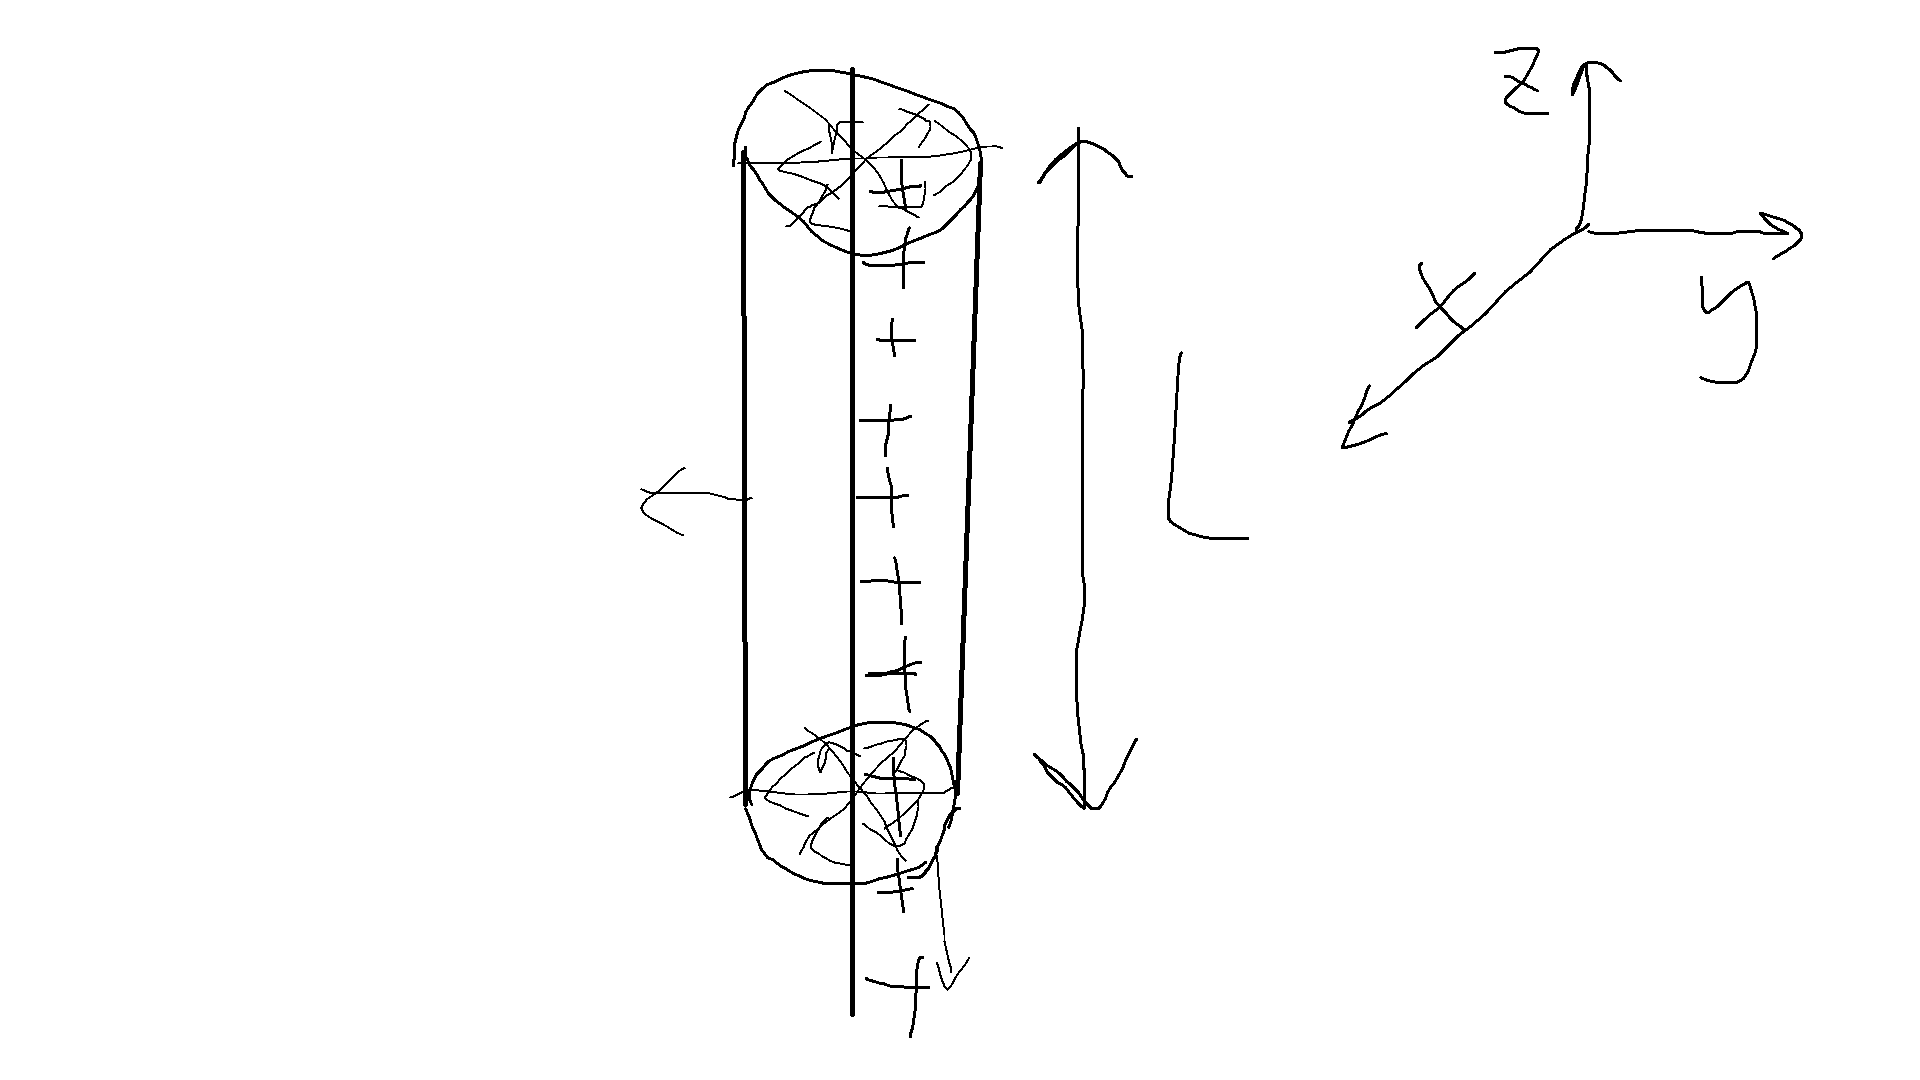
\includegraphics[scale=0.5]{EM_08}

By symmetry in cylindrical polars,
\begin{equation*}
\begin{aligned}
\mathbf{E}(\mathbf{r}) = E(r) \mathbf{\hat{r}}
\end{aligned}
\end{equation*}
where $r = \sqrt{x^2+y^2}$.

Take a cylinder of length $L$ with $d\mathbf{S} = \mathbf{\hat{r}} rd\phi dz$ while upper and lower disks with $d\mathbf{S} = \pm \mathbf{\hat{z}}r dr d\phi$ -- do not contribute as $\mathbf{\hat{z}} \cdot \mathbf{\hat{r}} = 0$. So
\begin{equation*}
\begin{aligned}
\int_S \mathbf{E} \cdot d\mathbf{S} &= E(r)2\pi r L\\
&=\eta \frac{L}{\varepsilon_0}
\end{aligned}
\end{equation*}
Hence we have our solution
\begin{equation*}\tag{2.5} \label{eq:2.5}
\begin{aligned}
E(r) = \frac{\eta}{2\pi \varepsilon_0} \frac{1}{r}
\end{aligned}
\end{equation*}
i.e. slower $\frac{1}{r}$ fall-off.

\end{eg}

\begin{eg} (Surface charge and matching conditions)\\
Suppose we have a charged plane at $z=0$. Charge density per unit area $\sigma(x,y)$. 

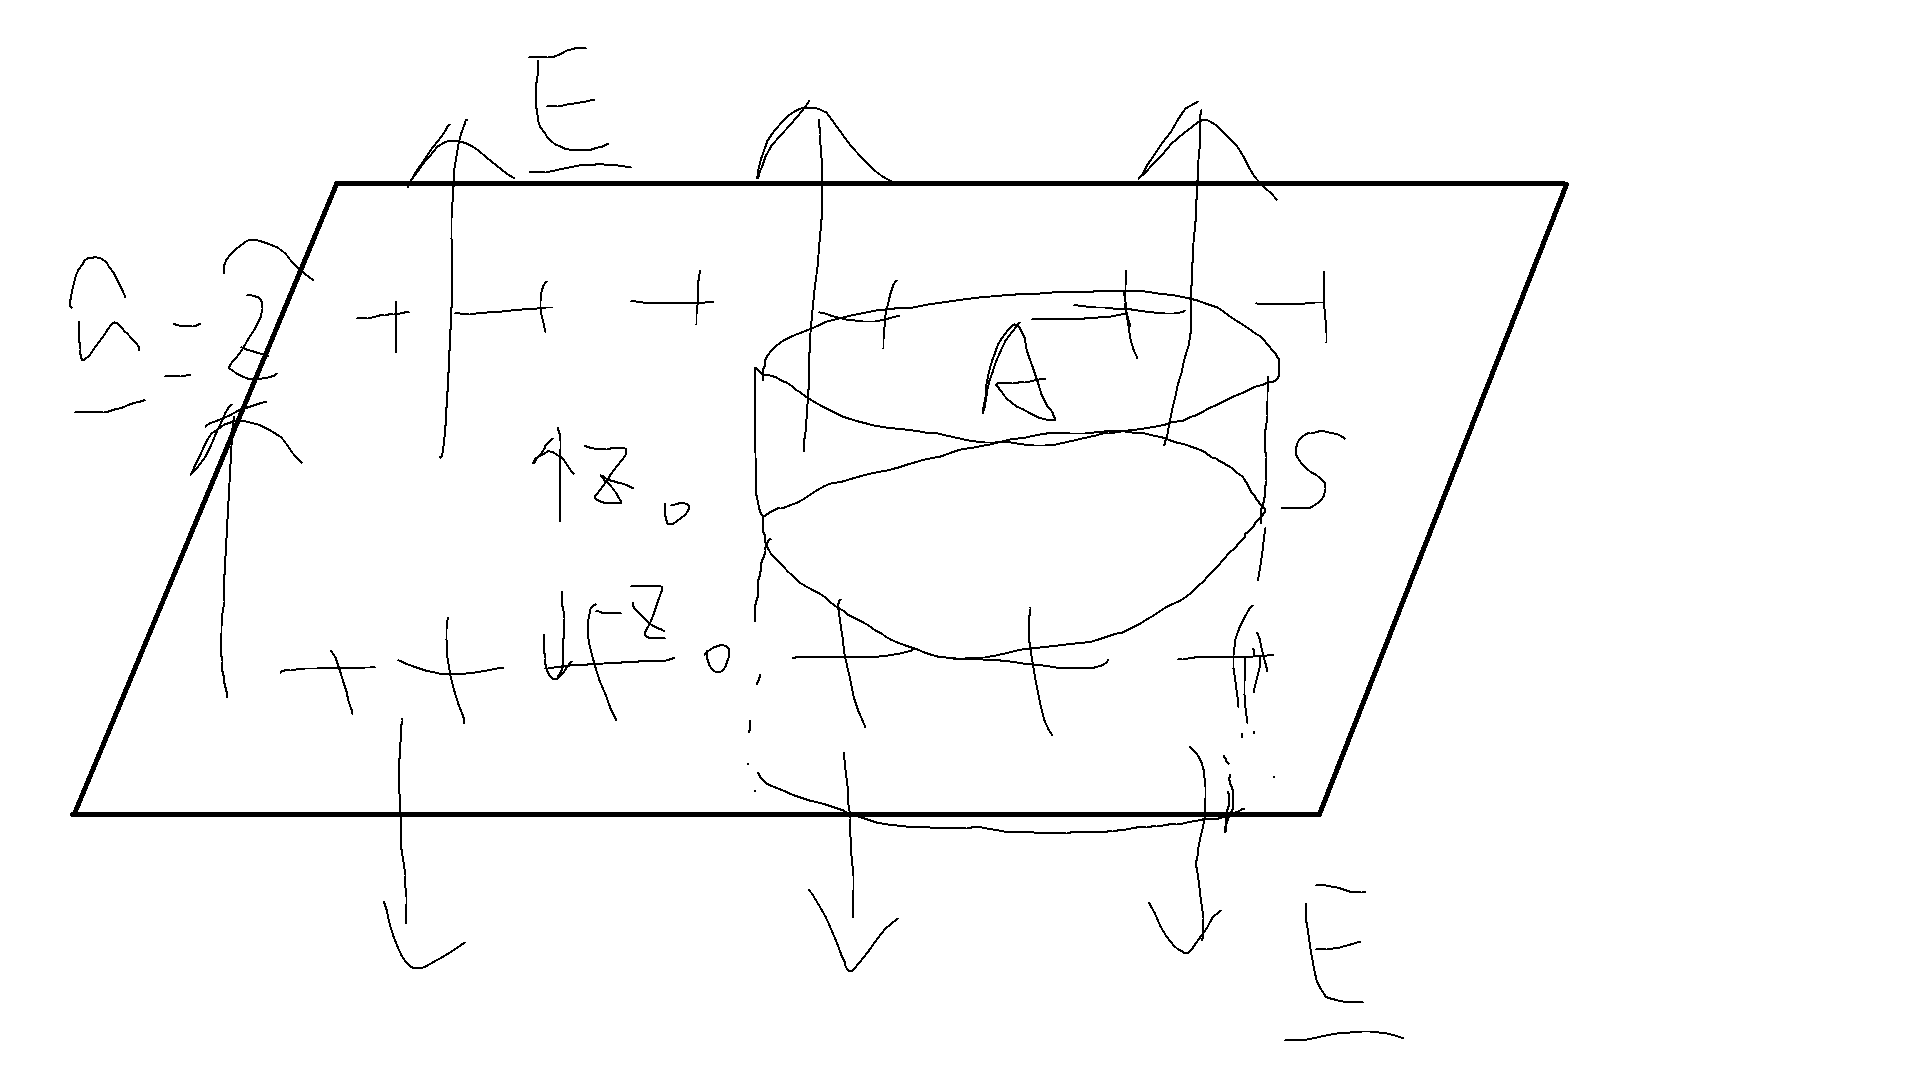
\includegraphics[scale=0.4]{EM_09}

By symmetry, we must have
\begin{equation*}
\begin{aligned}
E(\mathbf{r}) = E(z)\mathbf{\hat{z}}
\end{aligned}
\end{equation*}
and $E(z) =-E(-z)$.

Consider a small cylinder $S$ enclosing an area $A$ of the charged surface.

The surface integral becomes
\begin{equation*}
\begin{aligned}
\int \mathbf{E} \cdot d\mathbf{S} &= E(z_0) A\text{ (top disk)} - E(-z_0) A\text{ (bottom disk)} + \mathbf{\hat{z}} \cdot \mathbf{\hat{r}} \text{ (=0)}\\
&= 2 E(z_0) A\\
&=\frac{\sigma A}{\varepsilon_0}
\end{aligned}
\end{equation*}
by Gauss' Law (\eqref{eq:2.3}) charge inside $S$.

Hence
\begin{equation*}\tag{2.6} \label{eq:2.6}
\begin{aligned}
E(z) = \frac{\sigma}{2 \varepsilon_0} \ (z>0)
\end{aligned}
\end{equation*}
which is independent of $z-$ perpendicular distance.

So as we approach the surface ($z \to 0$), there is a discontinuity
\begin{equation*}\tag{2.7} \label{eq:2.7}
\begin{aligned}
E(z \to 0^+) - E(z \to 0^-) = \frac{\sigma}{\varepsilon_0}
\end{aligned}
\end{equation*}
This result is easy to \emph{generalize} to an arbitrary surface $S$ (with normal $\mathbf{\hat{n}}$) with inhomogeneous $\sigma$:

\begin{equation*}\tag{2.8} \label{eq:2.8}
\begin{aligned}
\mathbf{\hat{n}} \cdot [\mathbf{E}^+ - \mathbf{E}^-] = \frac{\sigma}{\varepsilon_0}
\end{aligned}
\end{equation*}
This is the \emph{matching condition} for the \emph{normal component} of $\mathbf{E}$.

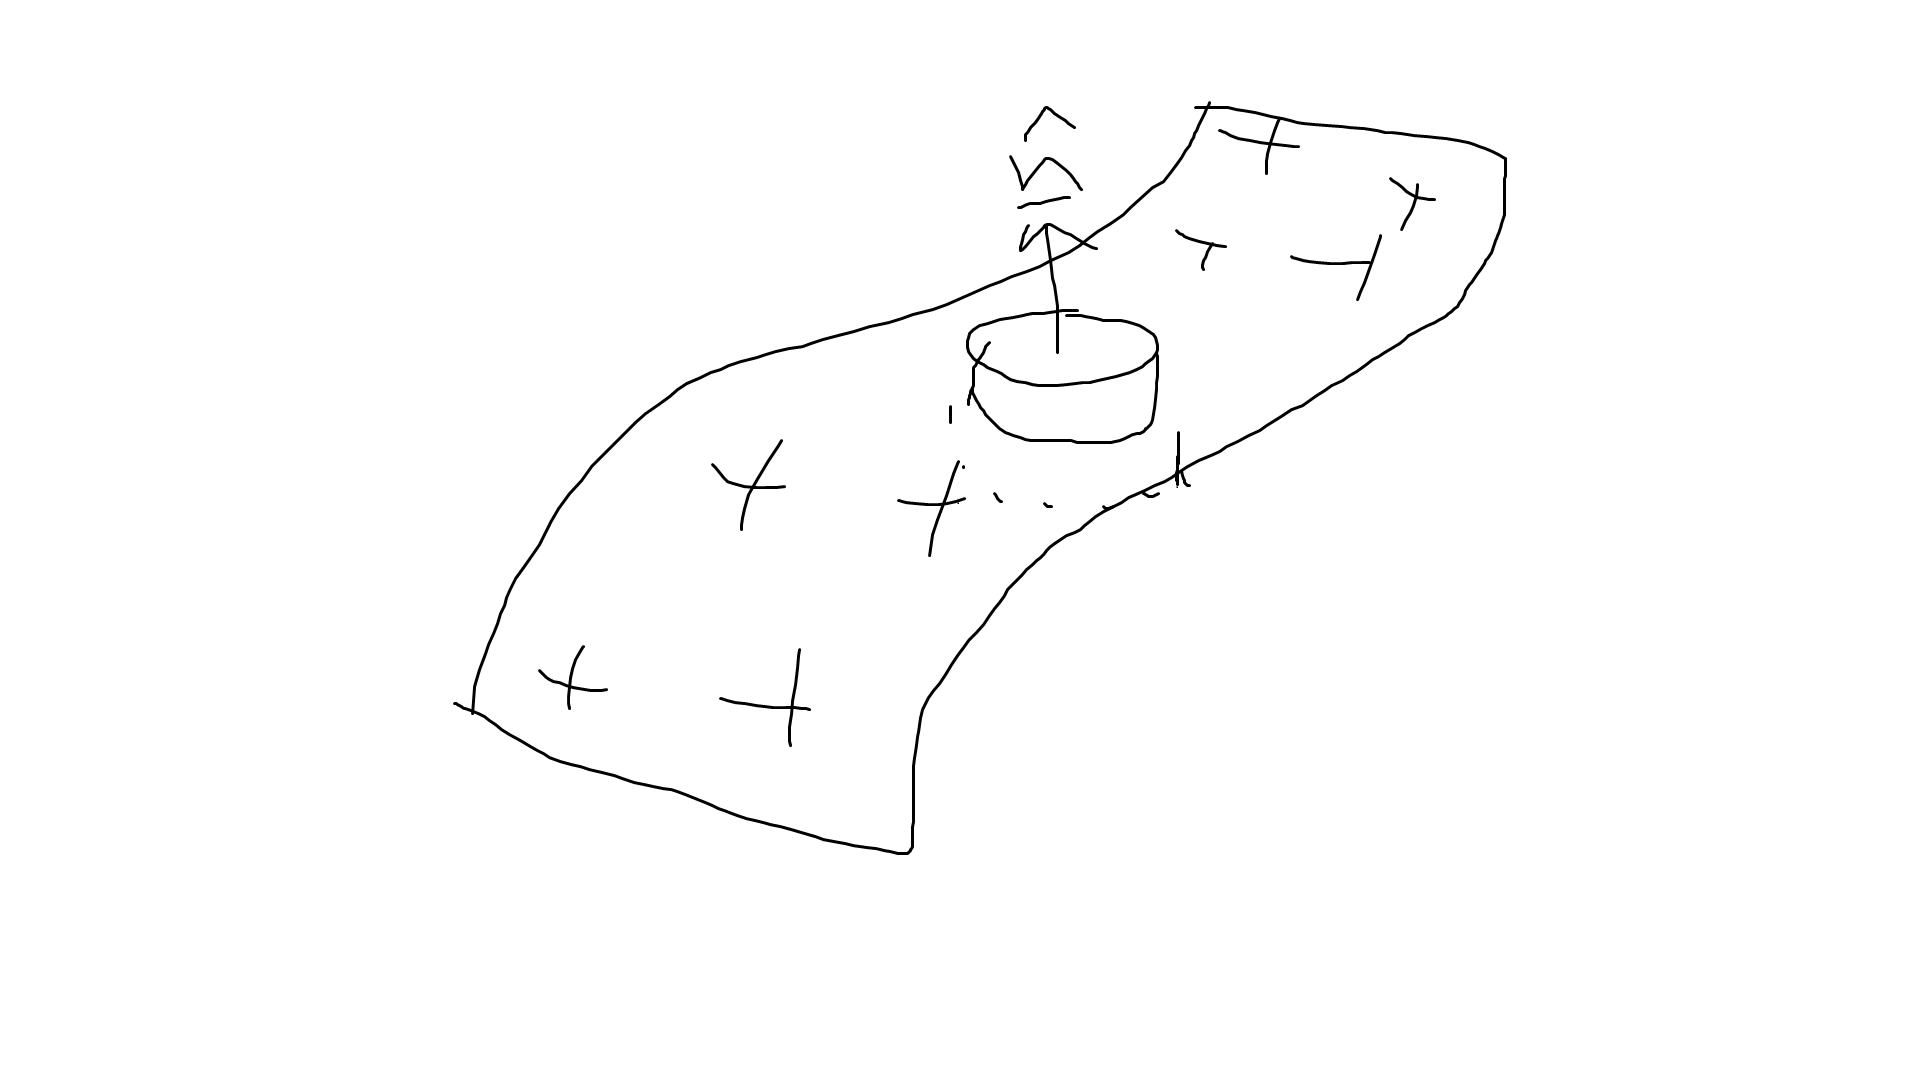
\includegraphics[scale=0.3]{EM_10}

Aside: Any field $\mathbf{E}$ on $S$ decomposes into normal $\mathbf{E}_\perp$ and tangential $\mathbf{E}_{//}$:
\begin{equation*}
\begin{aligned}
\mathbf{E} = \mathbf{E}_\perp + \mathbf{E}_{//} = (\mathbf{E} \cdot \mathbf{\hat{n}})\mathbf{\hat{n}} + \mathbf{E} - (\mathbf{E} \cdot \mathbf{n})\mathbf{\hat{n}} = (\mathbf{E} \cdot \mathbf{\hat{n}})\mathbf{\hat{n}} +\mathbf{\hat{n}} \times (\mathbf{E} \times \mathbf{\hat{n}})
\end{aligned}
\end{equation*}

We can show that the tangential component $\mathbf{E}_{//}$ on $S$ has to be continuous:
\begin{equation*}\tag{2.9} \label{eq:2.9}
\begin{aligned}
\mathbf{\hat{n}} \times [\mathbf{E}^+ - \mathbf{E}^-] = 0
\end{aligned}
\end{equation*}

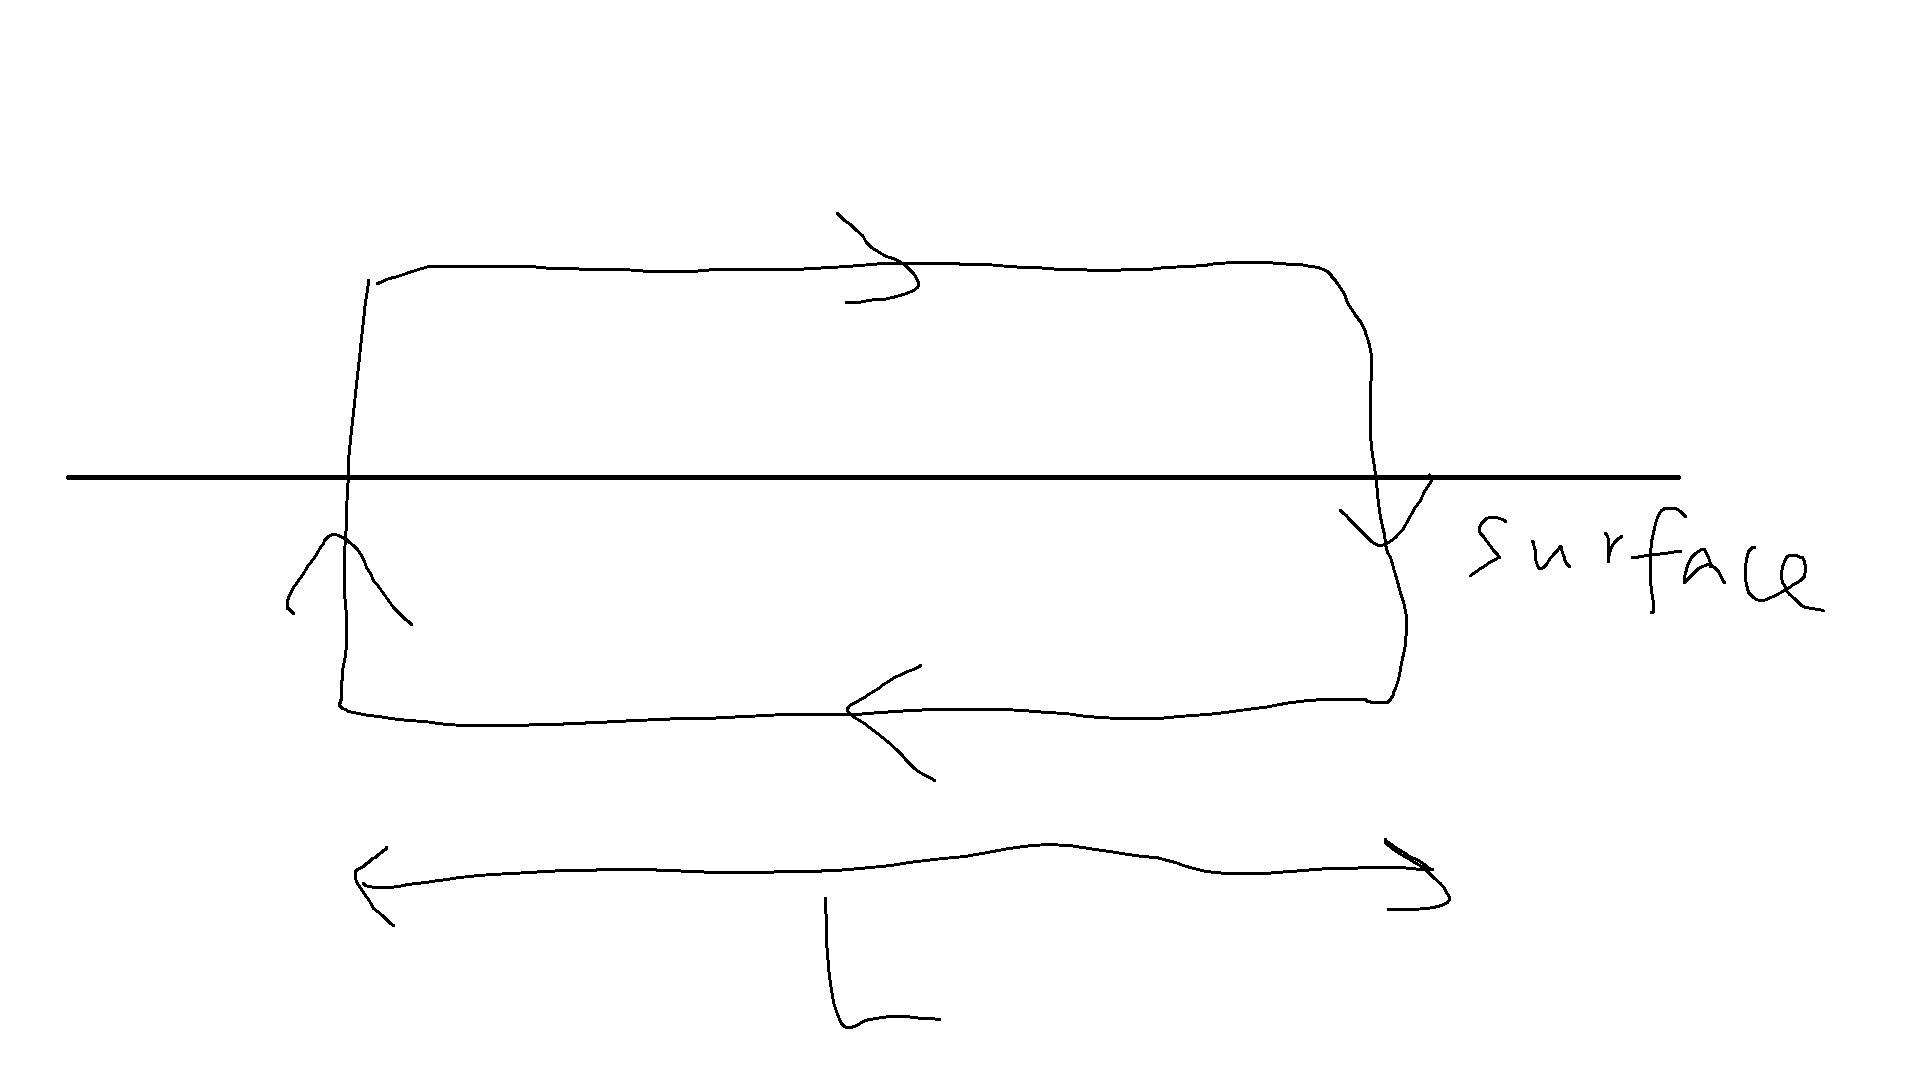
\includegraphics[scale=0.4]{EM_11}

This can be shown using the line integral
\begin{equation*}\tag{2.10} \label{eq:2.10}
\begin{aligned}
\oint \mathbf{E} \cdot d \mathbf{l} &= \int_S \nabla \times \mathbf{E} \cdot d \mathbf{S}\\
&= 0
\end{aligned}
\end{equation*}
By Stokes' Theorem and \eqref{eq:2.2} respectively (see David Tong's lecture notes).

\end{eg}

\begin{eg} 
Consider empty shell of radius $R$ with surface charge $\sigma$ with $Q = 4\pi R^2 \sigma$.

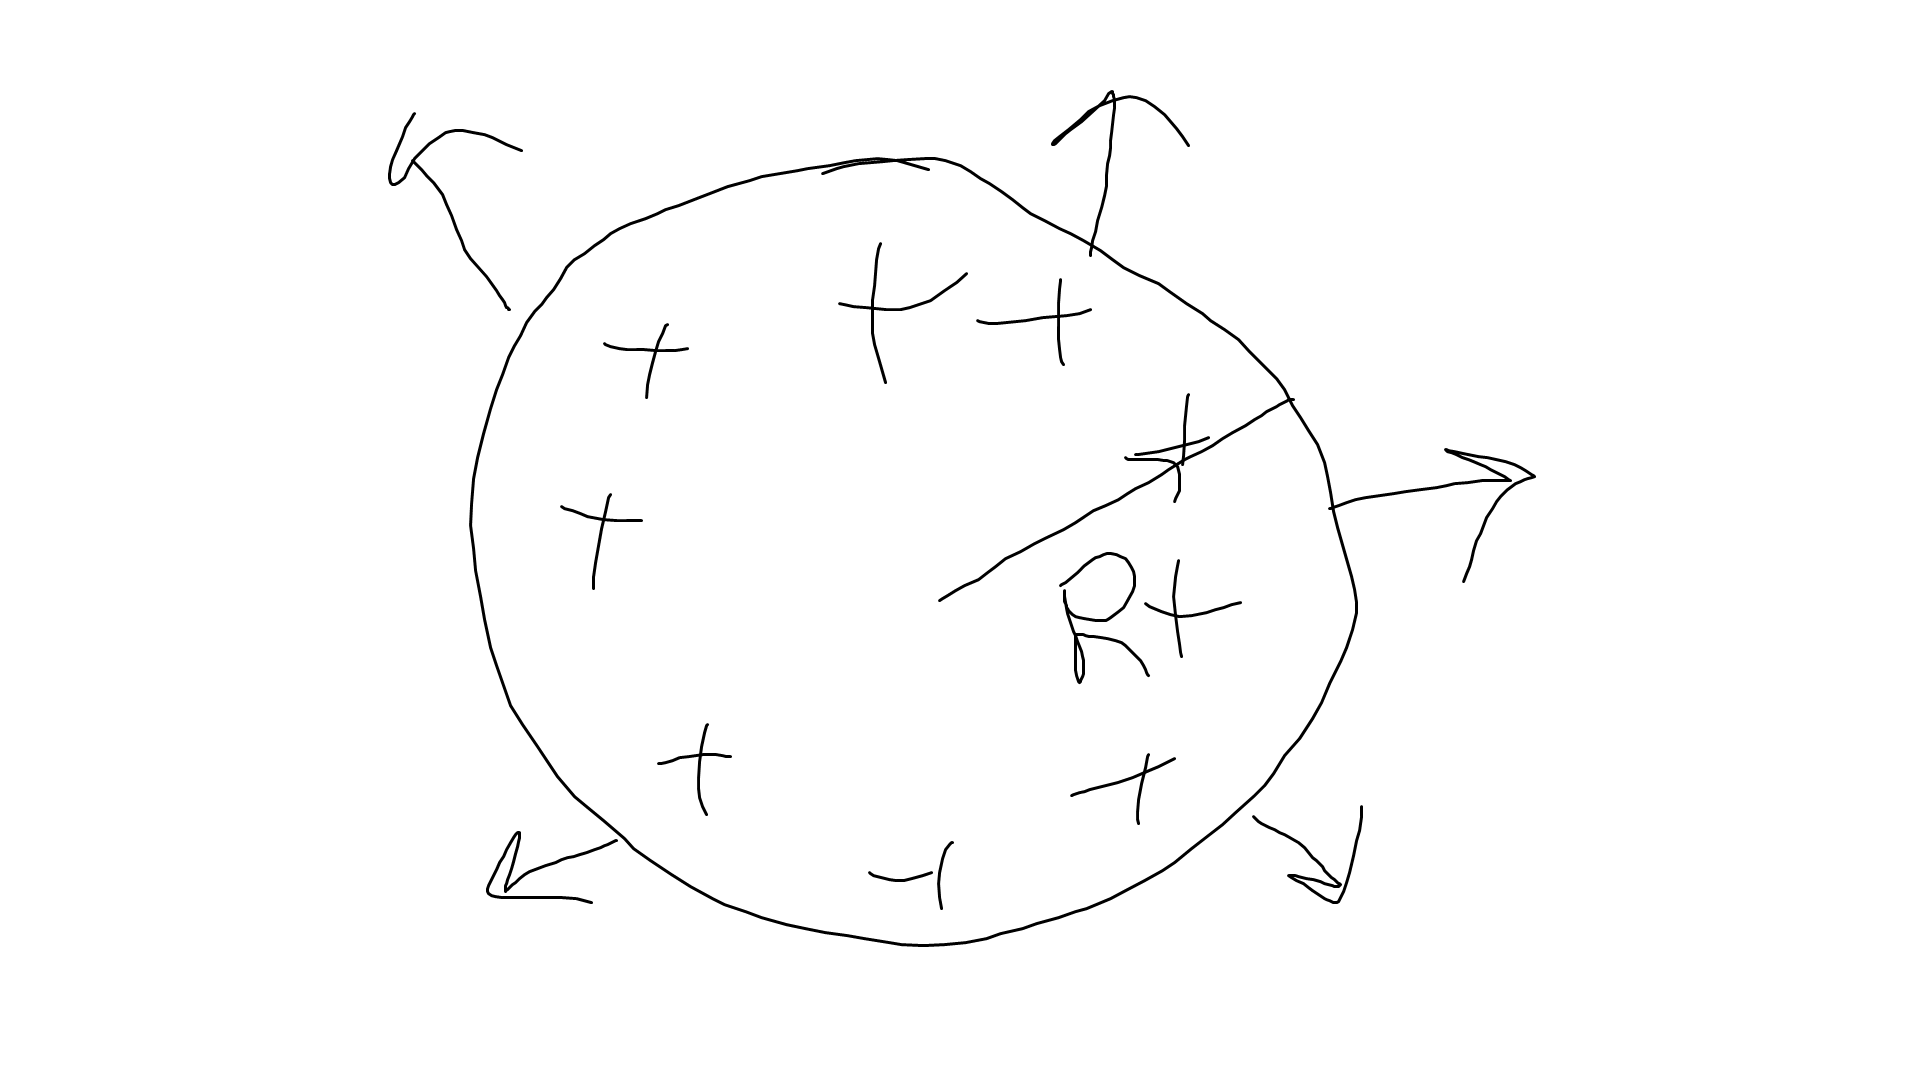
\includegraphics[scale=0.4]{EM_12}

This has the Coulomb solution
\begin{equation*}
\begin{aligned}
\mathbf{E} = \left\{ \begin{array}{ll}
\frac{1}{4\pi \varepsilon_0}\frac{Q}{r^2} \mathbf{\hat{r}} = \frac{r}{\varepsilon_0}\left(\frac{R}{r}\right)^2 & r>R\\
0 & r<R
\end{array}\right.
\end{aligned}
\end{equation*}

So $\mathbf{\hat{r}} \cdot (\mathbf{E}^+ - \mathbf{E}^-) =\frac{\sigma}{\varepsilon_0}$ at $r=R$ on surface $S$ satisfying \eqref{eq:2.6} - \eqref{eq:2.7}.
\end{eg}

\subsection{Electrostatic potential}
The scalar field is curl-free, i.e. $\nabla \times \mathbf{E} = 0$, so it can be expressed as the gradient of a scalar potential $\phi(\mathbf{x})$:
\begin{equation*}\tag{2.11} \label{eq:2.11}
\begin{aligned}
\mathbf{E} = -\nabla \phi
\end{aligned}
\end{equation*}
(Helmholtz decomposition: every differentiable vector field $\mathbf{F}$ can be decomposed into a curl-free and a divergence-free part, i.e. $\mathbf{F} = -\nabla \phi + \nabla \times \mathbf{A}$).

The electrostatic equation \eqref{eq:2.1} $\nabla \cdot \mathbf{E} = \frac{\rho}{\varepsilon_0}$ becomes the \emph{Poisson equation}
\begin{equation*}\tag{2.12} \label{eq:2.12}
\begin{aligned}
\nabla^2 \phi = -\frac{\rho}{\varepsilon_0}
\end{aligned}
\end{equation*}
If $\rho = 0$, the homogeneous form is the \emph{Laplace equation}
\begin{equation*}\tag{2.13} \label{eq:2.13}
\begin{aligned}
\nabla^2 \phi = 0
\end{aligned}
\end{equation*}

Both \eqref{eq:2.12},\eqref{eq:2.13} are linear, so we can use the \emph{superposition} of solution (e.g. $\rho = \rho_1+\rho_2$, $\phi = \phi_1 + \phi_2$ and $\mathbf{E} = \mathbf{E}_1+\mathbf{E}_2$) notably by employing summation over Green's functions.

\subsubsection{Point charge revisited}
Consider \eqref{eq:1.1} $\rho(\mathbf{r}) = q\delta (\mathbf{r})$, a point $q$ at $\mathbf{r} = 0$.
\begin{equation*}\tag{2.14} \label{eq:2.14}
\begin{aligned}
\nabla^2 \phi = -\frac{q}{\varepsilon_0} \delta(\mathbf{r})
\end{aligned}
\end{equation*}

The symmetric solution must have
\begin{equation*}
\begin{aligned}
\phi(\mathbf{r}) = \phi(r)
\end{aligned}
\end{equation*}
so use Gauss' Law on the interior of a sphere $S^2$ centred at $\mathbf{r} = 0$. (normal $\mathbf{\hat{n}} = \mathbf{\hat{r}}$):
\begin{equation*}
\begin{aligned}
\int_V \nabla^2 \phi d^3 \mathbf{r} &= \int_{S^2} \nabla \phi \cdot \mathbf{\hat{n}} (=\frac{d\phi}{dr}) dS\\
&=\frac{-q}{\varepsilon_0}
\end{aligned}
\end{equation*}
from \eqref{eq:2.14} with \eqref{eq:1.4}.\\
Hence, $4\pi r^2 \frac{d\phi}{dr} = -\frac{q}{\varepsilon_0}$, $\frac{d\phi}{dr} = \frac{-q}{4\pi \varepsilon_0}\frac{1}{r^2}$ yielding
\begin{equation*}\tag{2.15} \label{eq:2.15}
\begin{aligned}
\phi = \frac{1}{4\pi \varepsilon_0}\frac{q}{r} + \text{ const}
\end{aligned}
\end{equation*}
Assuming boundary conditions $\phi \to 0 $ as $r \to \infty$, then this is free-space Green's function (check Methods).

As before \eqref{eq:1.10}, the electric field is
\begin{equation*}
\begin{aligned}
\mathbf{E} = -\nabla \phi = \frac{1}{4\pi \varepsilon_0} \frac{q}{r^2} \mathbf{\hat{r}}.
\end{aligned}
\end{equation*}

\subsubsection{The Dipole}
Consider two particles with opposite charge with $-q$ at $\mathbf{r} = 0$ and $+q$ at $\mathbf{r} = \mathbf{d}$.

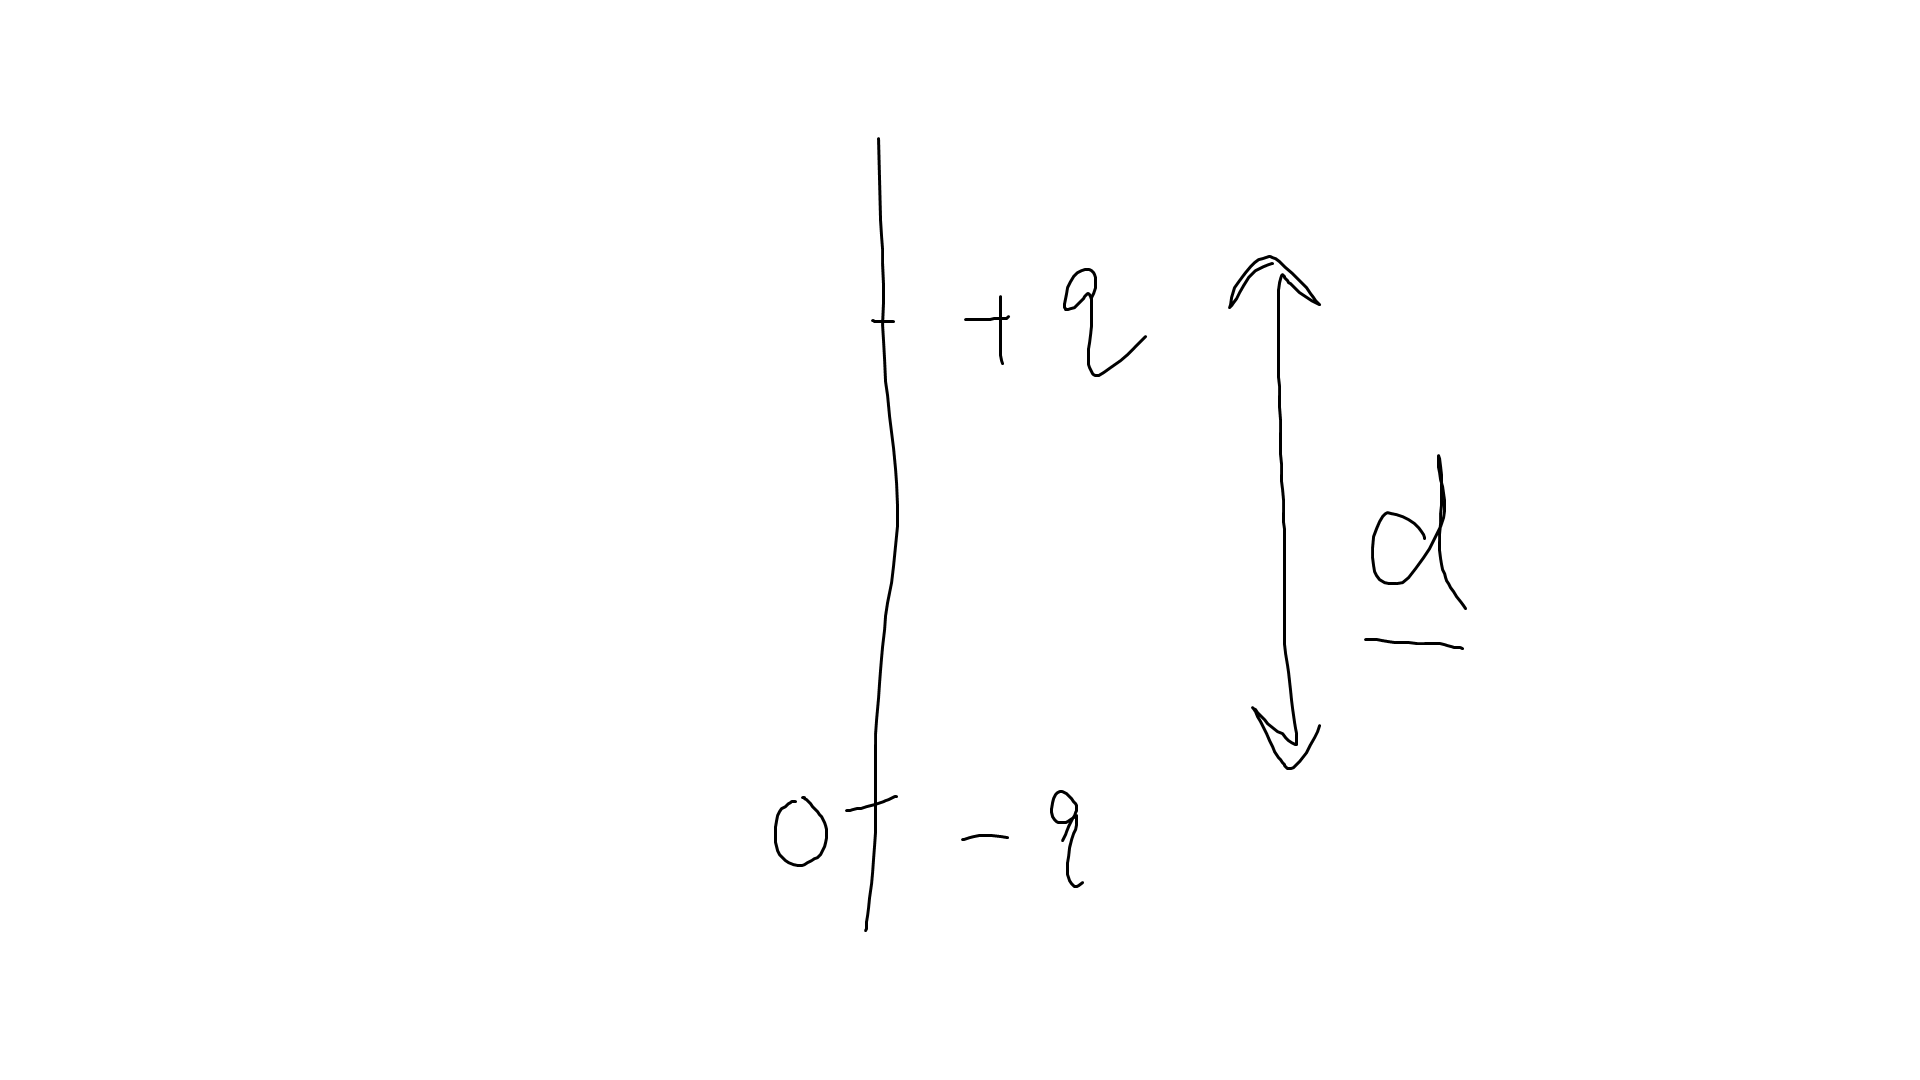
\includegraphics[scale=0.4]{EM_13}

By superposition of \eqref{eq:2.15}, the solution is simply
\begin{equation*}\tag{2.16} \label{eq:2.16}
\begin{aligned}
\phi(\mathbf{r}) = \frac{1}{4\pi \varepsilon_0} \left( \frac{-q}{r} + \frac{q}{|\mathbf{r} - \mathbf{d}|}\right)
\end{aligned}
\end{equation*}

Expanding in Taylor series
\begin{equation*}
\begin{aligned}
f(\mathbf{r}-\mathbf{d}) = f(\mathbf{r}) - \mathbf{d} \cdot \nabla f(\mathbf{r}) + \frac{1}{2}(\mathbf{d} \cdot \nabla)^2 f(\mathbf{r}) + ...
\end{aligned}
\end{equation*}
So
\begin{equation*}
\begin{aligned}
\frac{1}{|\mathbf{r} - \mathbf{d}|} &= \frac{1}{r} - \mathbf{d} \cdot \nabla\left(\frac{1}{r}\right) + \frac{1}{2}(\mathbf{d}\cdot \nabla)^2 \left(\frac{1}{r}\right)+...\\
&= \frac{1}{r} + \frac{\mathbf{d} \cdot \mathbf{r}}{r^3} - \frac{1}{2}\left(\frac{|\mathbf{d}|^2}{r^3} - \frac{3(\mathbf{d} \cdot \mathbf{r})^2}{r^5}\right)+...
\end{aligned}
\end{equation*}

So the dipole solution as $|\mathbf{r}| \to \infty$
\begin{equation*}
\begin{aligned}
\phi &= \frac{q}{4\pi \varepsilon_0} \left(-\frac{1}{r} + \frac{1}{r} + \frac{\mathbf{d} \cdot \mathbf{r}}{r^3} + ... \right)\\
&\approx \frac{q}{4\pi \varepsilon_0} \frac{\mathbf{d} \cdot \mathbf{r}}{r^3}.
\end{aligned}
\end{equation*}

Defining the \emph{dipole moment} $\mathbf{p} = q\mathbf{d}$ pointing from the negative to the positive charge, we have
\begin{equation*}\tag{2.17} \label{eq:2.17}
\begin{aligned}
\phi = \frac{\mathbf{p} \cdot \hat{\mathbf{r}}}{4\pi \varepsilon_0 r^2}
\end{aligned}
\end{equation*}

The dipole electric field is
\begin{equation*}\tag{2.18} \label{eq:2.18}
\begin{aligned}
\mathbf{E} = -\nabla \phi &= -\frac{1}{4\pi \varepsilon_0} \left((\mathbf{p} \cdot \mathbf{r}) \nabla \left(\frac{1}{r^3}\right) + \frac{\nabla(\mathbf{p} \cdot \mathbf{r})}{r^3}\right)\\
&=\frac{1}{4\pi \varepsilon_0} \left(\frac{3(\mathbf{p} \cdot \mathbf{r}) \hat{\mathbf{r}} - \mathbf{p}}{r^3}\right)
\end{aligned}
\end{equation*}

\subsubsection{General Green's function solution}
Recall that the Laplacian $\nabla^2 G(\mathbf{r};\mathbf{r}') = \delta(\mathbf{r}-\mathbf{r}')$ has the free-space Green's function
\begin{equation*}\tag{2.19} \label{eq:2.19}
\begin{aligned}
G(\mathbf{r},\mathbf{r}') = \frac{-1}{4\pi |\mathbf{r}-\mathbf{r'}|}
\end{aligned}
\end{equation*}
If we take charge distribution $\rho(\mathbf{r}) \neq 0$ only in a compact region $V \subset \R^3$.

Then the general solution for the Poisson equation \eqref{eq:2.12} is
\begin{equation*}\tag{2.20} \label{eq:2.20}
\begin{aligned}
\phi(r) &= \frac{-1}{\varepsilon_0} \int G(\mathbf{r};\mathbf{r'}) \rho(\mathbf{r'}) d^3 \mathbf{r}'\\
&= \frac{1}{4\pi \varepsilon_0} \int \frac{\rho(\mathbf{r'})}{|\mathbf{r}-\mathbf{r'}|} d^3 \mathbf{r'}
\end{aligned}
\end{equation*}
with electric field
\begin{equation*}\tag{2.21} \label{eq:2.21}
\begin{aligned}
\mathbf{E}(\mathbf{r}) = -\nabla \phi &= -\frac{1}{4\pi\varepsilon_0} \int \rho(\mathbf{r'})\nabla_\mathbf{r} \left(\frac{1}{|\mathbf{r}-\mathbf{r'}|}\right) d^3 \mathbf{r'}\\
&=\frac{1}{4\pi \varepsilon_0} \int \frac{\rho(\mathbf{r'}) (\mathbf{r}-\mathbf{r'})}{|\mathbf{r}-\mathbf{r'}|^3}d^3 \mathbf{r'}
\end{aligned}
\end{equation*}
Aside: If instead, Dirichlet boundary conditions imposed in the near(?) domain, then $$G(\mathbf{r};\mathbf{r'}) = -\frac{1}{4\pi |\mathbf{r}-\mathbf{r'}|} + H(\mathbf{r},\mathbf{r'})$$ where $H$ is harmonic and chosen so that $G=0$ on the boundary of $V$ (see Methods).

At far distances beyond $V$ (i.e. $\mathbf{r} \gg \mathbf{r'}, \forall \mathbf{r'}$), the solution \eqref{eq:2.20} becomes
\begin{equation*}\tag{2.22} \label{eq:2.22}
\begin{aligned}
\phi(\mathbf{r}) &= \frac{1}{4\pi \varepsilon_0} \int d^3 \mathbf{r'} \rho(\mathbf{r'}) \left(\frac{1}{r} + \frac{\mathbf{r} \cdot \mathbf{r'}}{r^3} + ...\right)\\
&= \frac{1}{4\pi \varepsilon_0} \left(\frac{Q}{r} + \frac{\mathbf{R} \cdot \hat{\mathbf{r}}}{r^2} + ...\right)
\end{aligned}
\end{equation*}
where total charge is \eqref{eq:1.6}
\begin{equation*}
\begin{aligned}
Q=\int d^3\mathbf{r'} \rho(\mathbf{r'})
\end{aligned}
\end{equation*}
and the average dipole moment is
\begin{equation*}\tag{2.23} \label{eq:2.23}
\begin{aligned}
\mathbf{p} = \int d^3 \mathbf{r'} \mathbf{r'} \rho(\mathbf{r}')
\end{aligned}
\end{equation*}
We can continue to expand to quadruple and higher moments.

\subsubsection{Equipotentials and field lines}
Move particle (charge $q$) along path $\mathbf{l}$ from $\mathbf{r}$ to $\mathbf{r'}$ in a potential $\phi(\mathbf{r})$. Potential energy $U$ given by work done against force $\mathbf{F} = q\mathbf{E} =-q\nabla \phi$:
\begin{equation*}\tag{2.24} \label{eq:2.24}
\begin{aligned}
U &= -\int_\mathbf{r}^\mathbf{r'} \mathbf{F} \cdot d\mathbf{l}\\
&= -q\int_\mathbf{r}^\mathbf{r'} \mathbf{E}\cdot d\mathbf{l}\\
&= q\int_\mathbf{r}^\mathbf{r'} \nabla\phi \cdot d\mathbf{l}\\
&= q[\phi(\mathbf{r'}) - \phi(\mathbf{r})]
\end{aligned}
\end{equation*}
i.e. the potential difference between $\mathbf{r}$ and $\mathbf{r'}$.

Recall that any line integral $\int \mathbf{E} \cdot d\mathbf{l}$ along a closed curve is $0$ since $\mathbf{E}$ is conservative.

Suppose that $\phi(\mathbf{r}) = \phi(\mathbf{r'}) =\phi_0$ along the path $\mathbf{l}$ from $\mathbf{r}$ to $\mathbf{r'}$, field satisfies
\begin{equation*}\tag{2.25} \label{eq:2.25}
\begin{aligned}
\phi(\mathbf{r})=\phi_0
\end{aligned}
\end{equation*}
which is a constant, thus defining a set of \emph{equipotential surfaces}.

Since $\int \mathbf{E}\cdot d\mathbf{l} = 0$, this implies $\mathbf{E}=0$ or $\mathbf{E}$ is normal to the surface. \emph{Electric field lines} are continuous lines drawn tangent to $\mathbf{E}(\mathbf{r})$ with density proportional to $|\mathbf{E}|$.

\begin{eg}
\emph{Point charges} field lines begin at the positive charge and end at the negative charge.

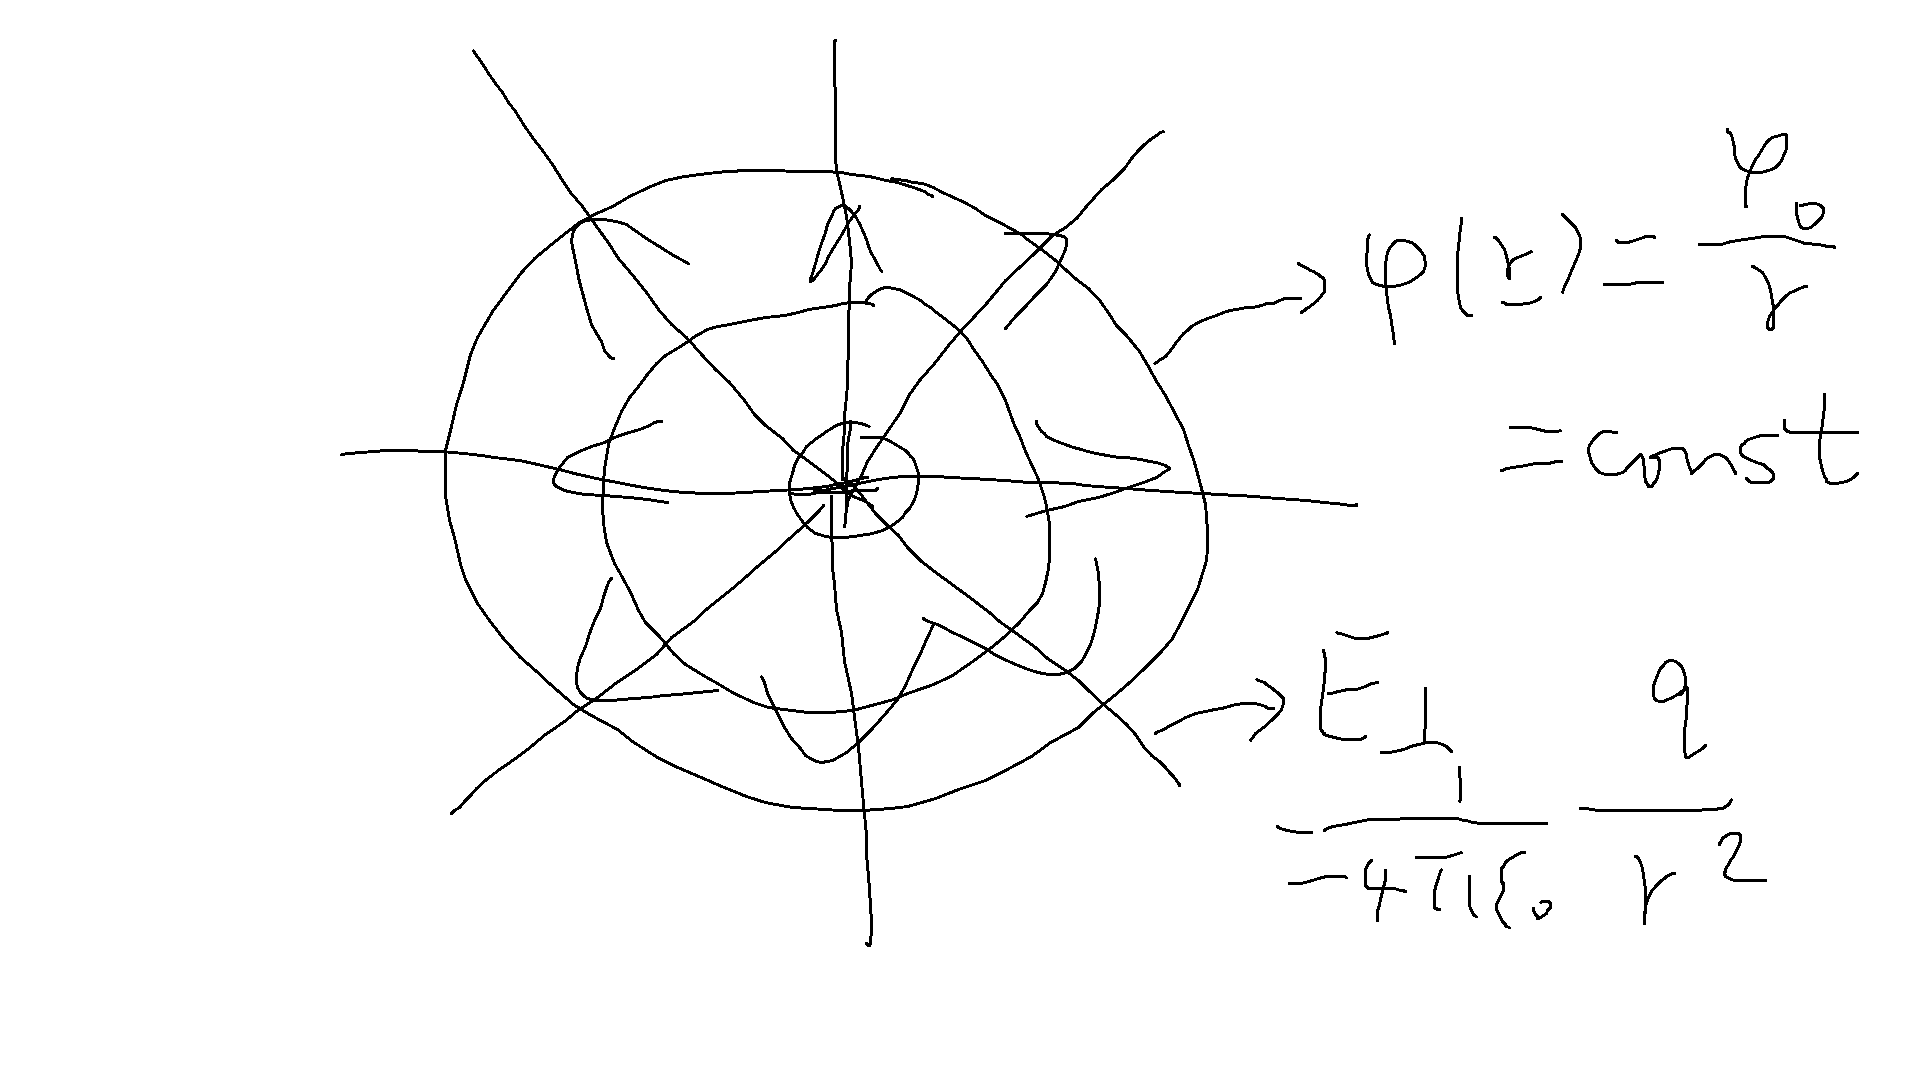
\includegraphics[scale=0.4]{EM_14}

and similarly for the negative charge.
\end{eg}

\begin{eg}
Consider a pure dipole \eqref{eq:2.17}.

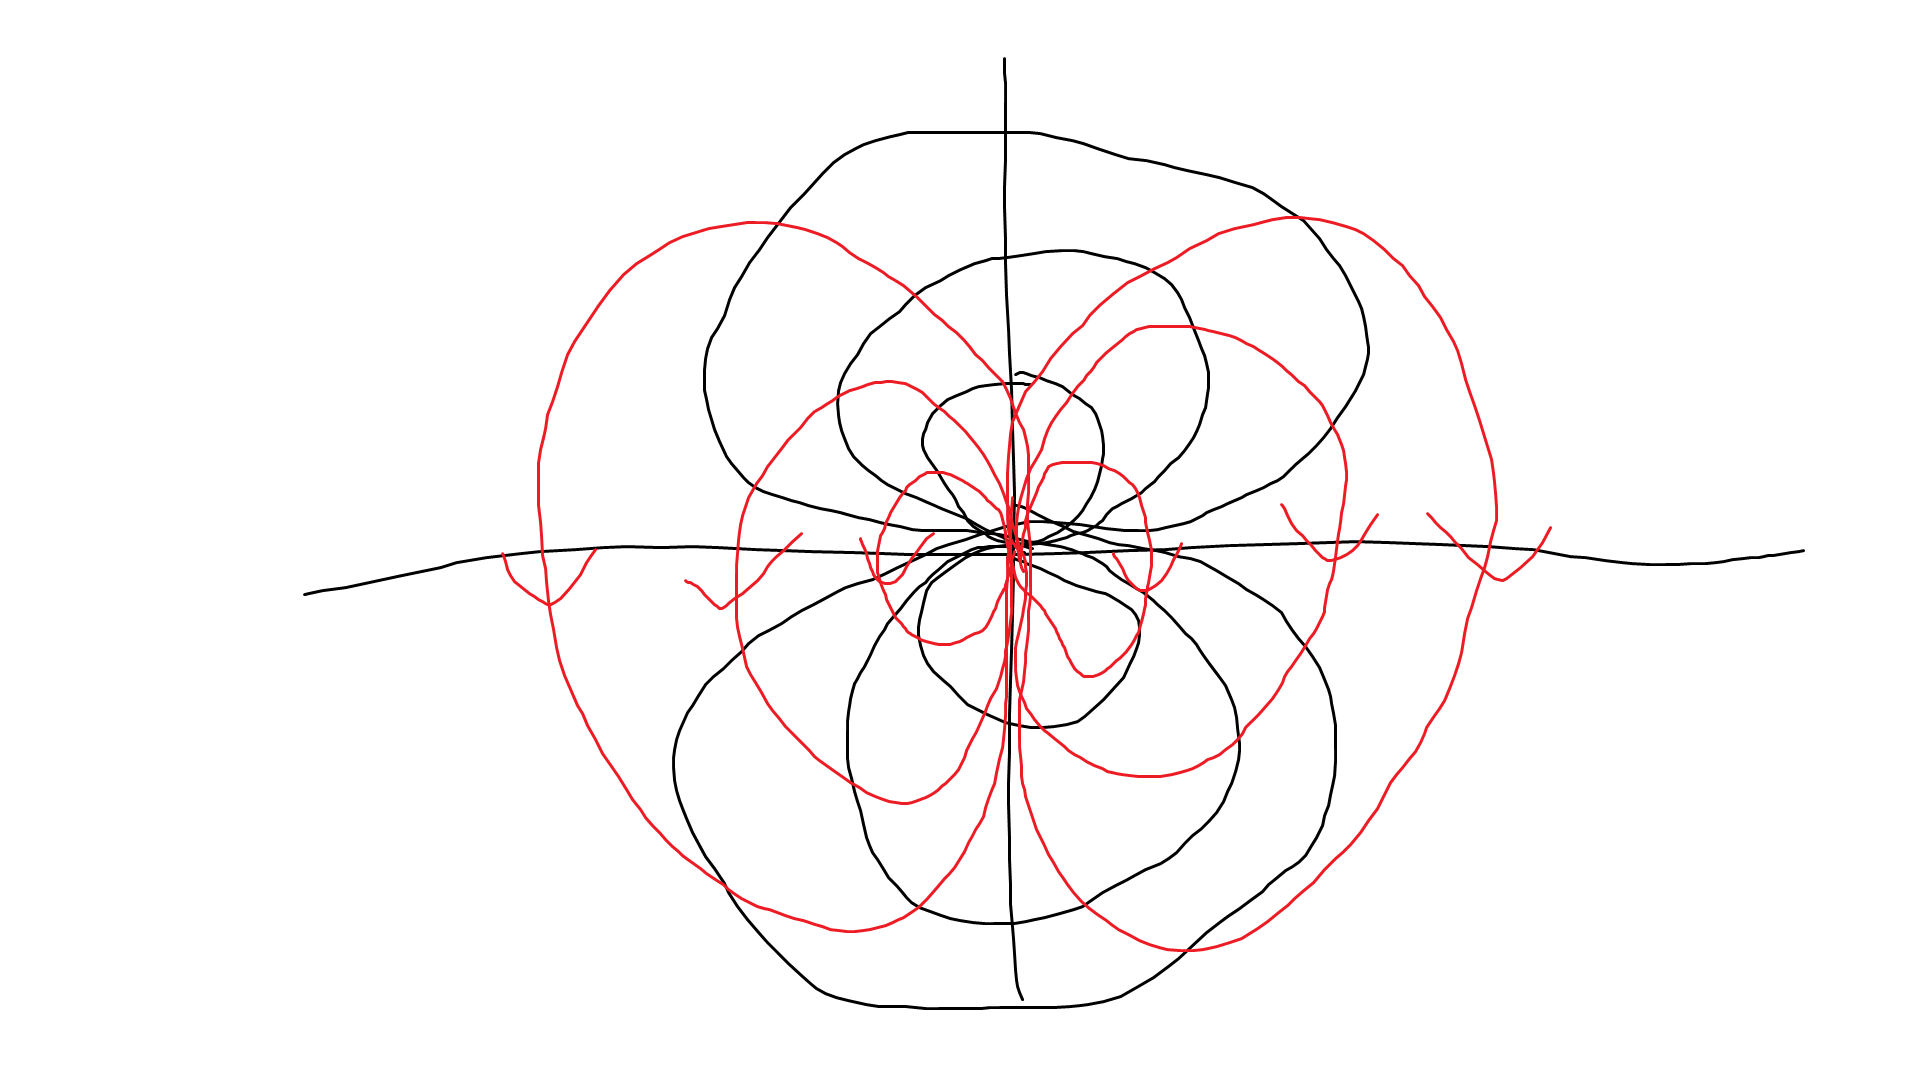
\includegraphics[scale=0.4]{EM_15}

where $\phi = \frac{\rho \cos \theta}{4\pi \varepsilon_0 r^2}$, $r \sim (\cos\theta)^{1/2}$, $E = \frac{1}{4\pi\varepsilon_0 r^2} [2\cos\theta \hat{\mathbf{r}}+\sin\theta \hat{\mathbf{\theta}}]$.
\end{eg}

\begin{eg}
The actual dipole is a combination of the above two.

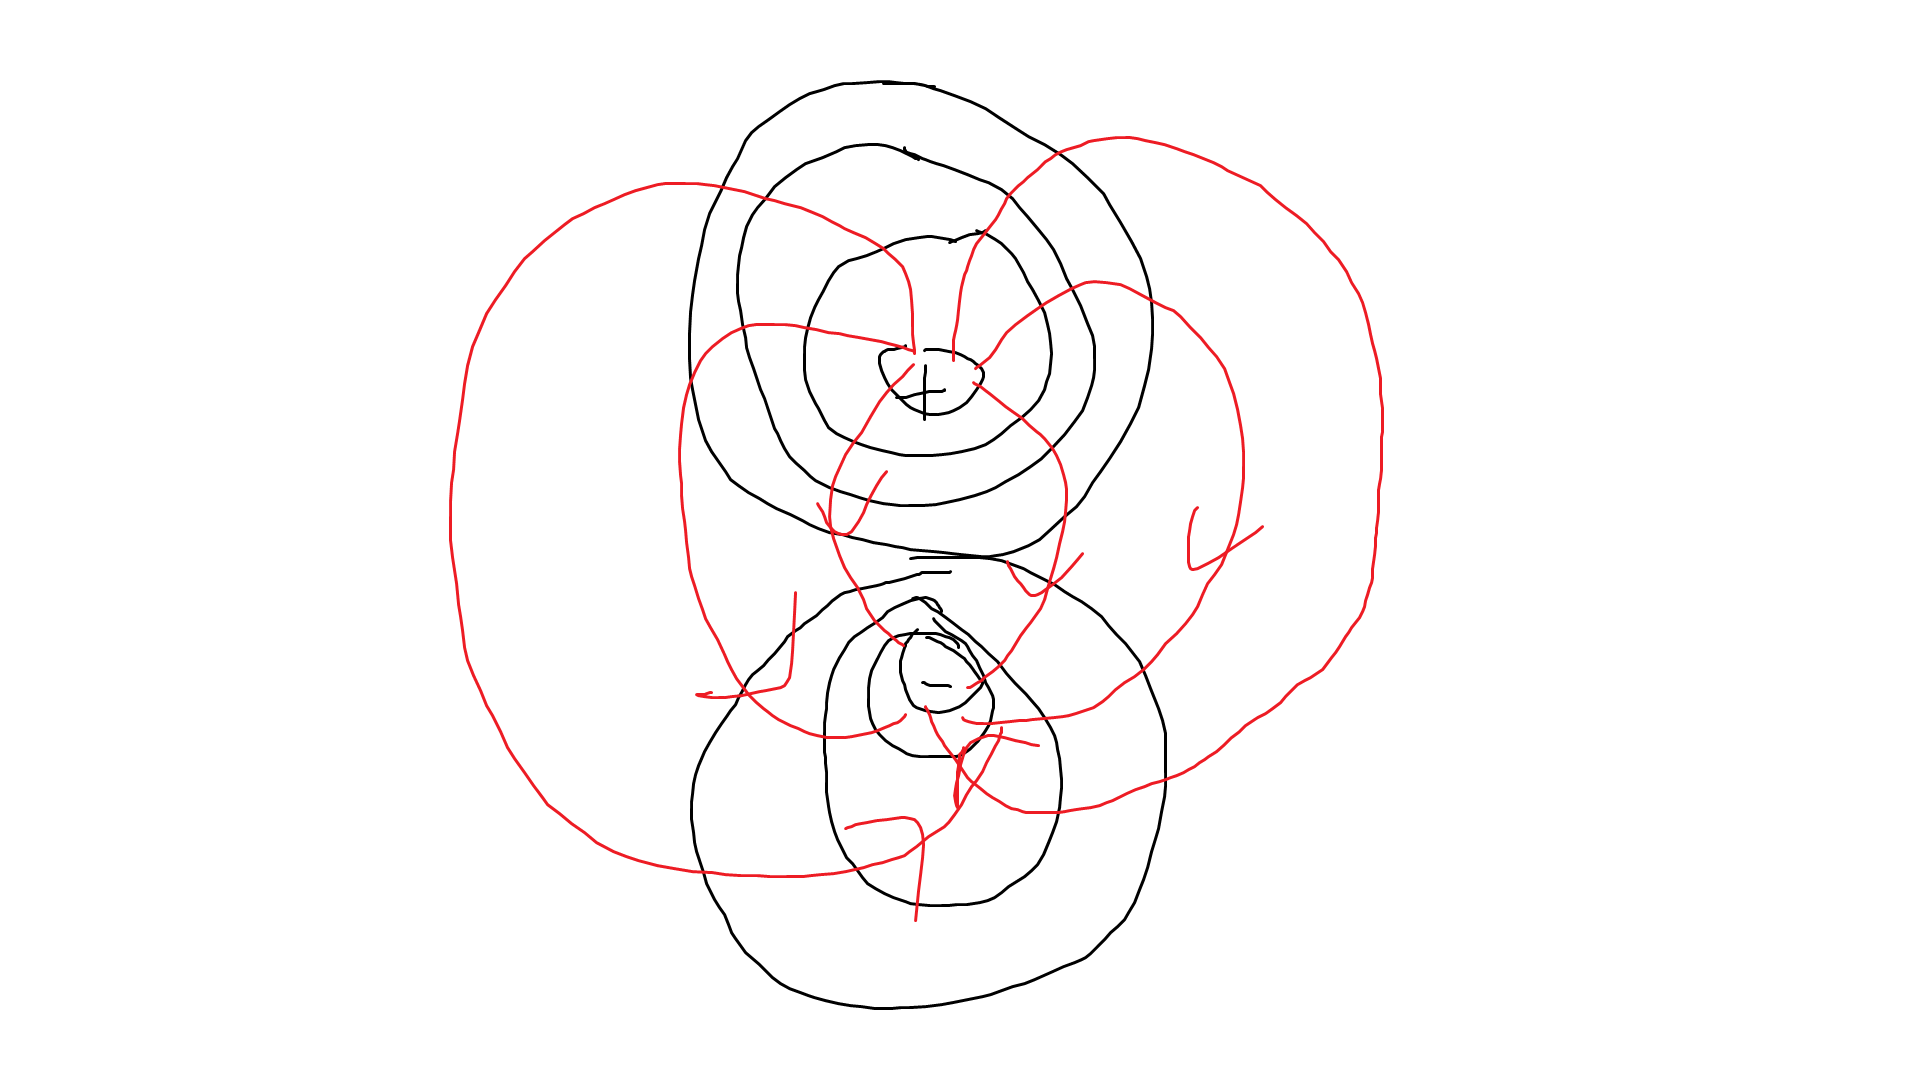
\includegraphics[scale=0.4]{EM_16}
\end{eg}

\subsection{Electrostatic energy}
How much electrostatic energy do $N$ charged particles have?

Place first particle (charge $q_1$, position $\mathbf{r}$) which creates potential
\begin{equation*}
\begin{aligned}
\phi_1(\mathbf{r}) = \frac{q_1}{4\pi \varepsilon_0|\mathbf{r}-\mathbf{r}_1|}
\end{aligned}
\end{equation*}
but we do no work $W=0$, i.e. we ignore the rest mass energy $E=mc^2$ of all particles (self energy).

Bring second particle from $r=\infty$ to $\mathbf{r} = \mathbf{r}_2$ yielding potential energy
\begin{equation*}
\begin{aligned}
W_2 = q[\phi_1 (\mathbf{r}_2) - \phi_1 (\infty)] = q_2 \phi_1 (\mathbf{r}_2) = \frac{q_1q_2}{4\pi \varepsilon_0 |\mathbf{r}_2 - \mathbf{r}_1|}
\end{aligned}
\end{equation*}

Bring third particle from $r=\infty$:
\begin{equation*}
\begin{aligned}
W_3 &= q_3[\phi_2 (\mathbf{r}_2) + \phi_1 (\mathbf{r}_1)]\\
&= q_3 \left(\frac{q_2}{|\mathbf{r_3}-\mathbf{r_2}|}+\frac{q_1}{|\mathbf{r_3}-\mathbf{r_1}|}\right)
\end{aligned}
\end{equation*}
etc.

Summing over all particles, the total PE is
\begin{equation*}\tag{2.26} \label{eq:2.26}
\begin{aligned}
U &= \sum_{i=1}^N W_i\\
&= \frac{1}{4\pi \varepsilon_0} \sum_{i=1}^n \sum_{j>i}^N \frac{q_i q_j}{|\mathbf{r}_i-\mathbf{r}_j|}\\
&= \frac{1}{8\pi\varepsilon_0} \sum_{i=1}^n \sum_{j \neq i}^n \frac{q_i q_j}{|\mathbf{r}_i-\mathbf{r}_j|}\\
&= \frac{1}{2} \sum_{i=1}^N \phi_i (\mathbf{r}_i)
\end{aligned}
\end{equation*}
where we define $\phi_i (\mathbf{r}_i) = \frac{1}{4\pi \varepsilon_0} \sum_{j\neq i} \frac{q_j}{|\mathbf{r}_i-\mathbf{r}_j|}$.

Now consider the continuous limit of electrostatic energy \eqref{eq:2.26}:
\begin{equation*}
\begin{aligned}
U = \frac{1}{2} \int_V d^3 \mathbf{r} \rho(\mathbf{r})\phi(\mathbf{r}) = \frac{\varepsilon_0}{2} \int_V d^3 \mathbf{r} (\nabla \cdot \mathbf{E}) \phi
\end{aligned}
\end{equation*}
by Maxwell's equation \eqref{eq:2.1}. This is then equal to
\begin{equation*}\tag{*}
\begin{aligned}
\frac{\varepsilon_0}{2} \int_V d^3 \mathbf{r} [\nabla(\mathbf{E}\phi)-\mathbf{E} \cdot \nabla \phi]
\end{aligned}
\end{equation*}
using $\nabla \cdot (\mathbf{E}\phi) = \nabla\cdot\mathbf{E} \ \phi + \mathbf{E} \cdot \nabla \phi$.

But by divergence theorem
\begin{equation*}
\begin{aligned}
\int_V \nabla \cdot (\mathbf{E}\phi) d^3 \mathbf{r} = \int_S \phi \mathbf{E} \cdot d\mathbf{S} \to 0
\end{aligned}
\end{equation*}
as $r \to \infty$, since on surface $S$, $\phi, E \to 0$ as $r \to \infty$ (for isolated charges $\phi \sim \frac{1}{r}, E\sim \frac{1}{r^2}, A \sim 4\pi r^2$, so $\int_S \to \frac{1}{r^3}r\pi r^2 \to 0$).

Using $\mathbf{E} = -\nabla \phi$, we find that (*) becomes
\begin{equation*}\tag{2.27} \label{eq:2.27}
\begin{aligned}
U = \frac{\varepsilon_0}{2} \int d^3 \mathbf{r} \mathbf{E} \cdot \mathbf{E}
\end{aligned}
\end{equation*}
i.e. equivalent to the \emph{energy of the electric field}.

\subsection{Conductors}
There are broadly 3 types of electrical materials:
$\bullet$ \emph{Insulators} have \emph{bound electrons} with a large energy gap to the conduction band;\\
$\bullet$ \emph{Semiconductors} have \emph{limited} numbers of absent electrons ('holes') which can move;\\
$\bullet$ \emph{Conductors} have \emph{many free electrons} in a conduction band and current flows freely.

For \emph{electrostatics} conductors have spherical properties:\\
$\bullet$ Any \emph{interior electric field must vanish}: $\mathbf{E} = 0$, otherwise electrons would move.\\
$\bullet$ Since interior $\mathbf{E} = 0$, from $\mathbf{E} = -\nabla \phi$ we know $\phi=$constant inside (equipotential).\\
$\bullet$ By $\nabla \cdot \mathbf{E} = \rho/\varepsilon_0$, there is no interior charge, i.e. $\rho = 0$ (despite there are many free electrons).\\
$\bullet$ Where have all the charges gone? They must all reside on the surface $S$ (with normal $\hat{\mathbf{n}}$.\\
$\bullet$ describe with \emph{surface charge density} $\sigma$.\\
$\bullet$ Any \emph{electric field} $E$ must be normal to conductor surface $S$ (any tangential field $\mathbf{E}_{//}$ would move charges).

By matching conditions (\eqref{eq:2.8}), the exterior field is
\begin{equation*}\tag{2.28} \label{eq:2.28}
\begin{aligned}
\mathbf{E} = \sigma/\varepsilon_0 \hat{\mathbf{n}}
\end{aligned}
\end{equation*}
i.e. Conductors define boundary conditions for the Poisson and Laplace's equations (\eqref{eq:2.12},\eqref{eq:2.13}).

\subsubsection{Electrostatic shielding (Faraday cage)}
The potential is constant inside the conductor $\phi_c=$constant, so true also in the cavity (region $V$).

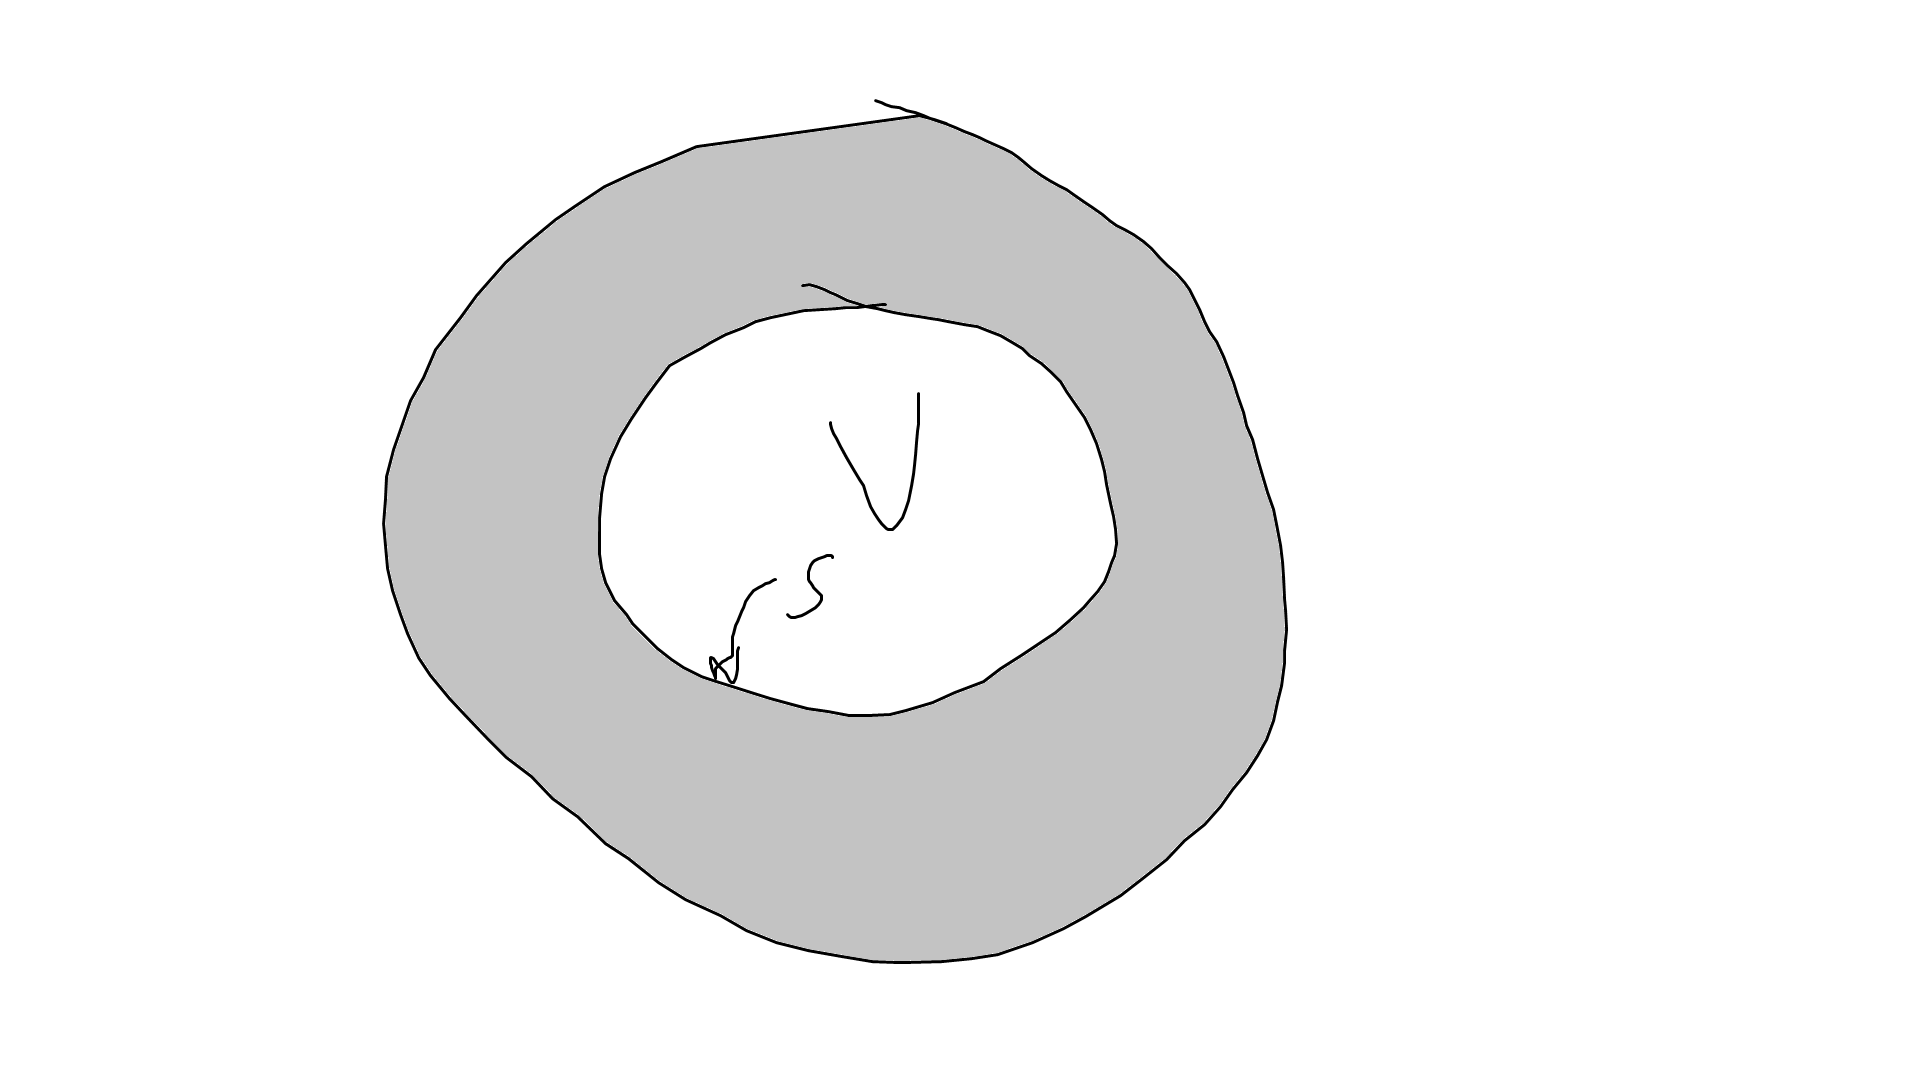
\includegraphics[scale=0.4]{EM_17}

Since the potential satisfies Laplace's equation $\nabla^2 \phi = 0$ we have $\mathbf{E} = 0$ inside cavity and no surface charge.

\textbf{Exercise.} Place charge $Q$ inside and show that it will be shielded by equal opposite charge on $S$.

\subsection{Method of images}
Conductors provide equipotential boundary conditions which, if sufficiently symmetric, can be satisfied instead by adding additional image or mirror charges. The \emph{uniqueness theorem} for solutions of Poisson's equation given $\rho$ and boundary conditions on $V$ means that any solution that satisfies these is the unique solution.

\begin{eg}
Consider a point charge $q$, a distance $z_0$ from a conducting plane at $z=0$ which is \emph{grounded or earthed} (i.e. is held at $\phi=0$).

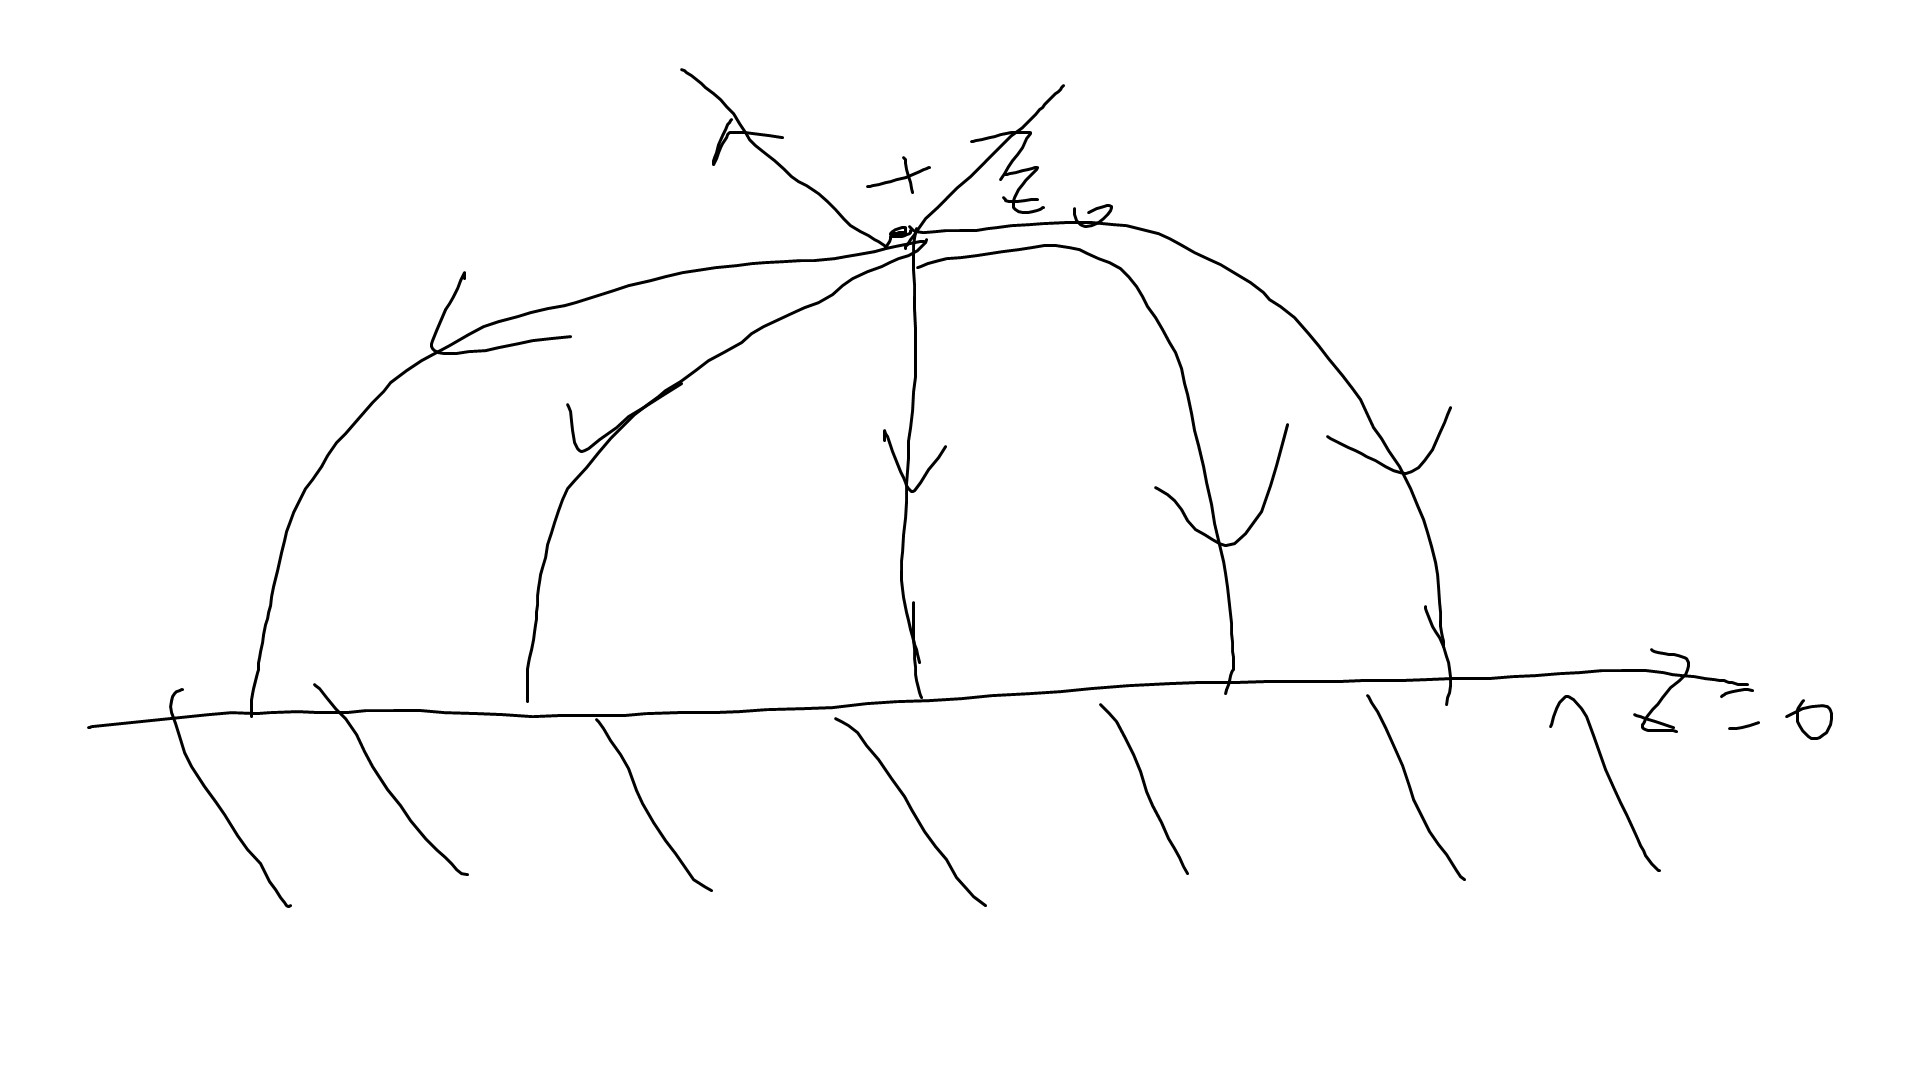
\includegraphics[scale=0.4]{EM_18}

Now instead of the conductor, place an image charge at $z=-z_0$.

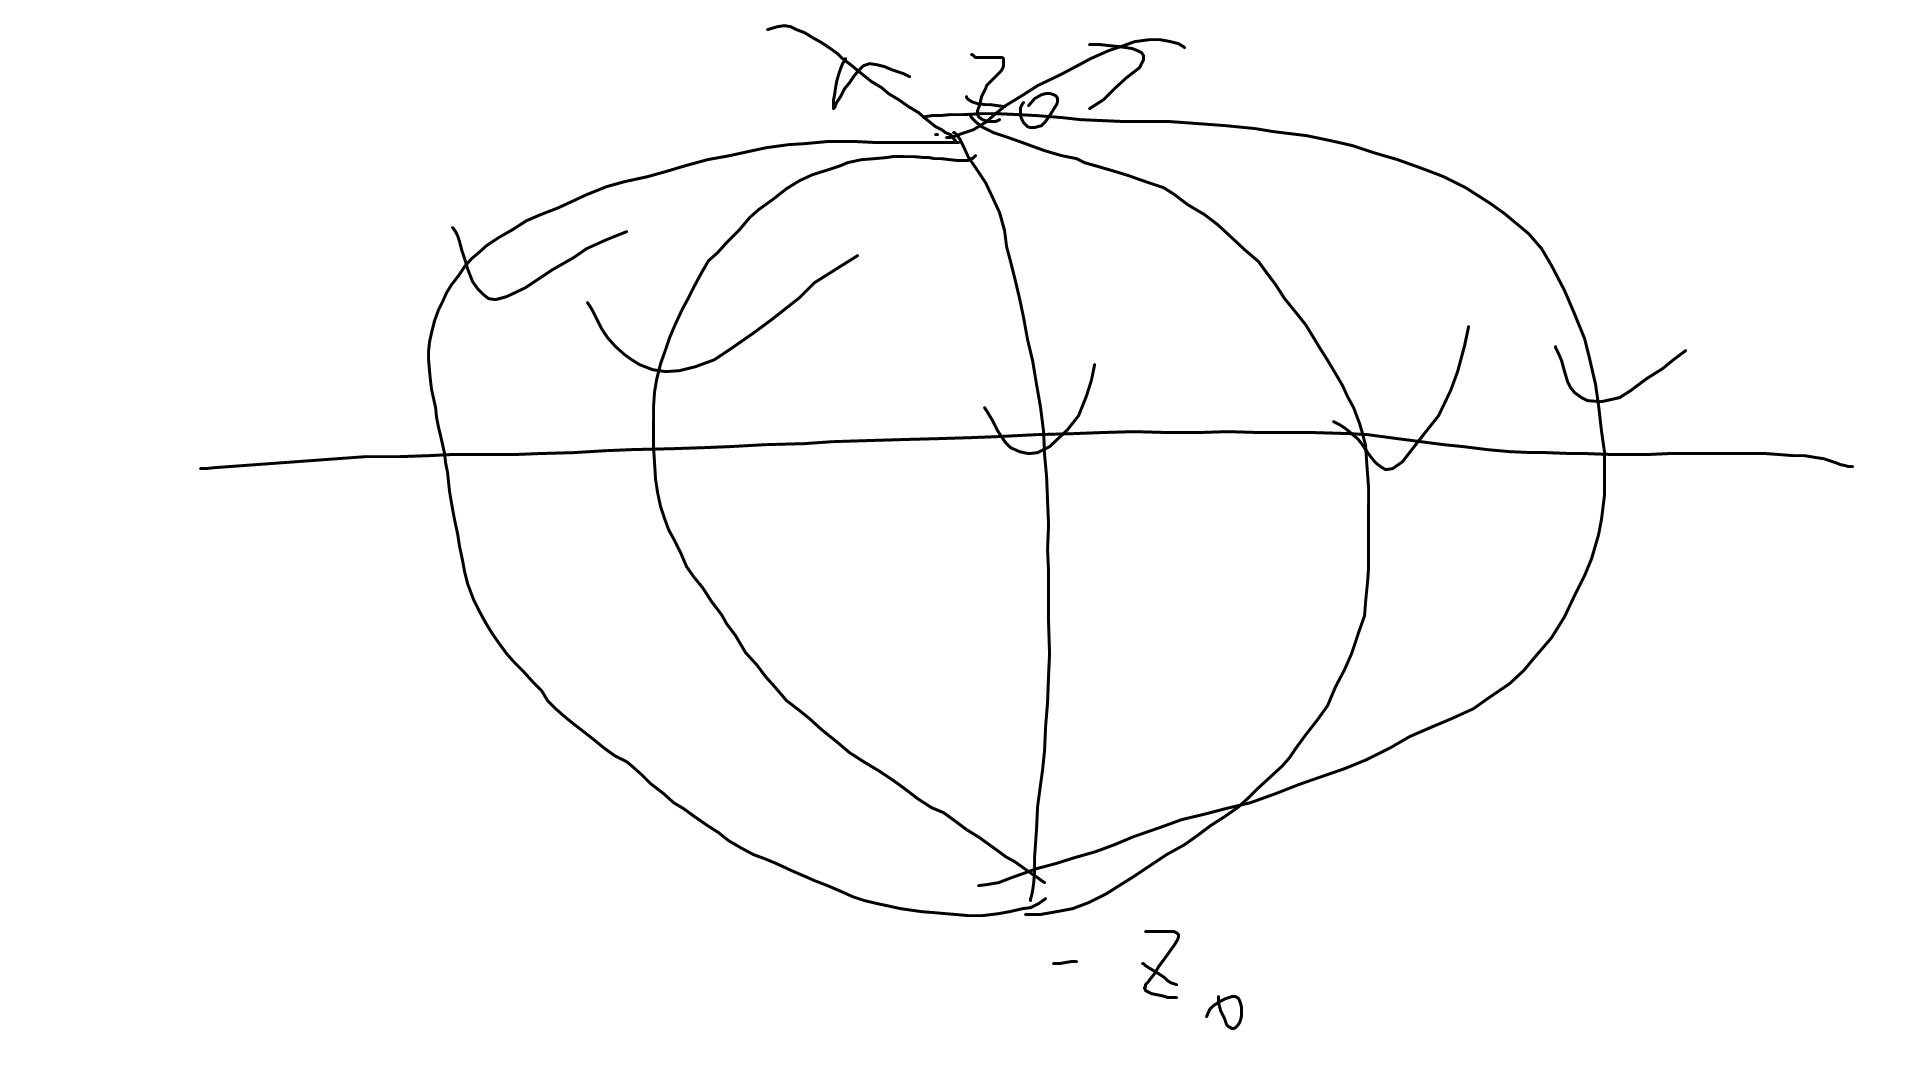
\includegraphics[scale=0.4]{EM_19}

The mirror solution is
\begin{equation*} 
\begin{aligned}
\phi = \frac{1}{4\pi \varepsilon_0} \left(\frac{q}{\sqrt{x^2+y^2 + (z-z_0)^2}}- \frac{q}{\sqrt{x^2 + y^2 + (z+z_0)^2}}\right)
\end{aligned}
\end{equation*}
for which it is clear that $\phi=0$ on the plane $z=0$.

Thus we also have the unique solution for $z>0$. Normal field $E_z$ is given by
\begin{equation*}\tag{2.29} \label{eq:2.29}
\begin{aligned}
E_z = -\frac{\partial \phi}{\partial z} = \frac{q}{4\pi \varepsilon} \left(\frac{z-z_0}{(x^2+y^2+(z-z_0)^2)^\frac{3}{2}} - \frac{z+z_0}{(x^2+y^2+(z+z_0)^2)^\frac{3}{2}} \right)
\end{aligned}
\end{equation*}
This induces a surface charge at $z=0$ from \eqref{eq:2.28} $E=\frac{\sigma}{\varepsilon_0} \hat{\mathbf{n}}$ given by
\begin{equation*}\tag{2.31} \label{eq:2.31}
\begin{aligned}
\sigma = \varepsilon_0 E_z|_{z=0} = \frac{q}{2\pi} \frac{z_0}{(x^2+y^2+z_0^2)^\frac{3}{2}}
\end{aligned}
\end{equation*}
\end{eg}

\textbf{Exercise.} Show that the total induced surface charge
\begin{equation*}
\begin{aligned}
Q=\int dxdy\sigma = -q
\end{aligned}
\end{equation*}
i.e. the same as the image charge.

\begin{eg} (Conducting sphere in an electric field)\\

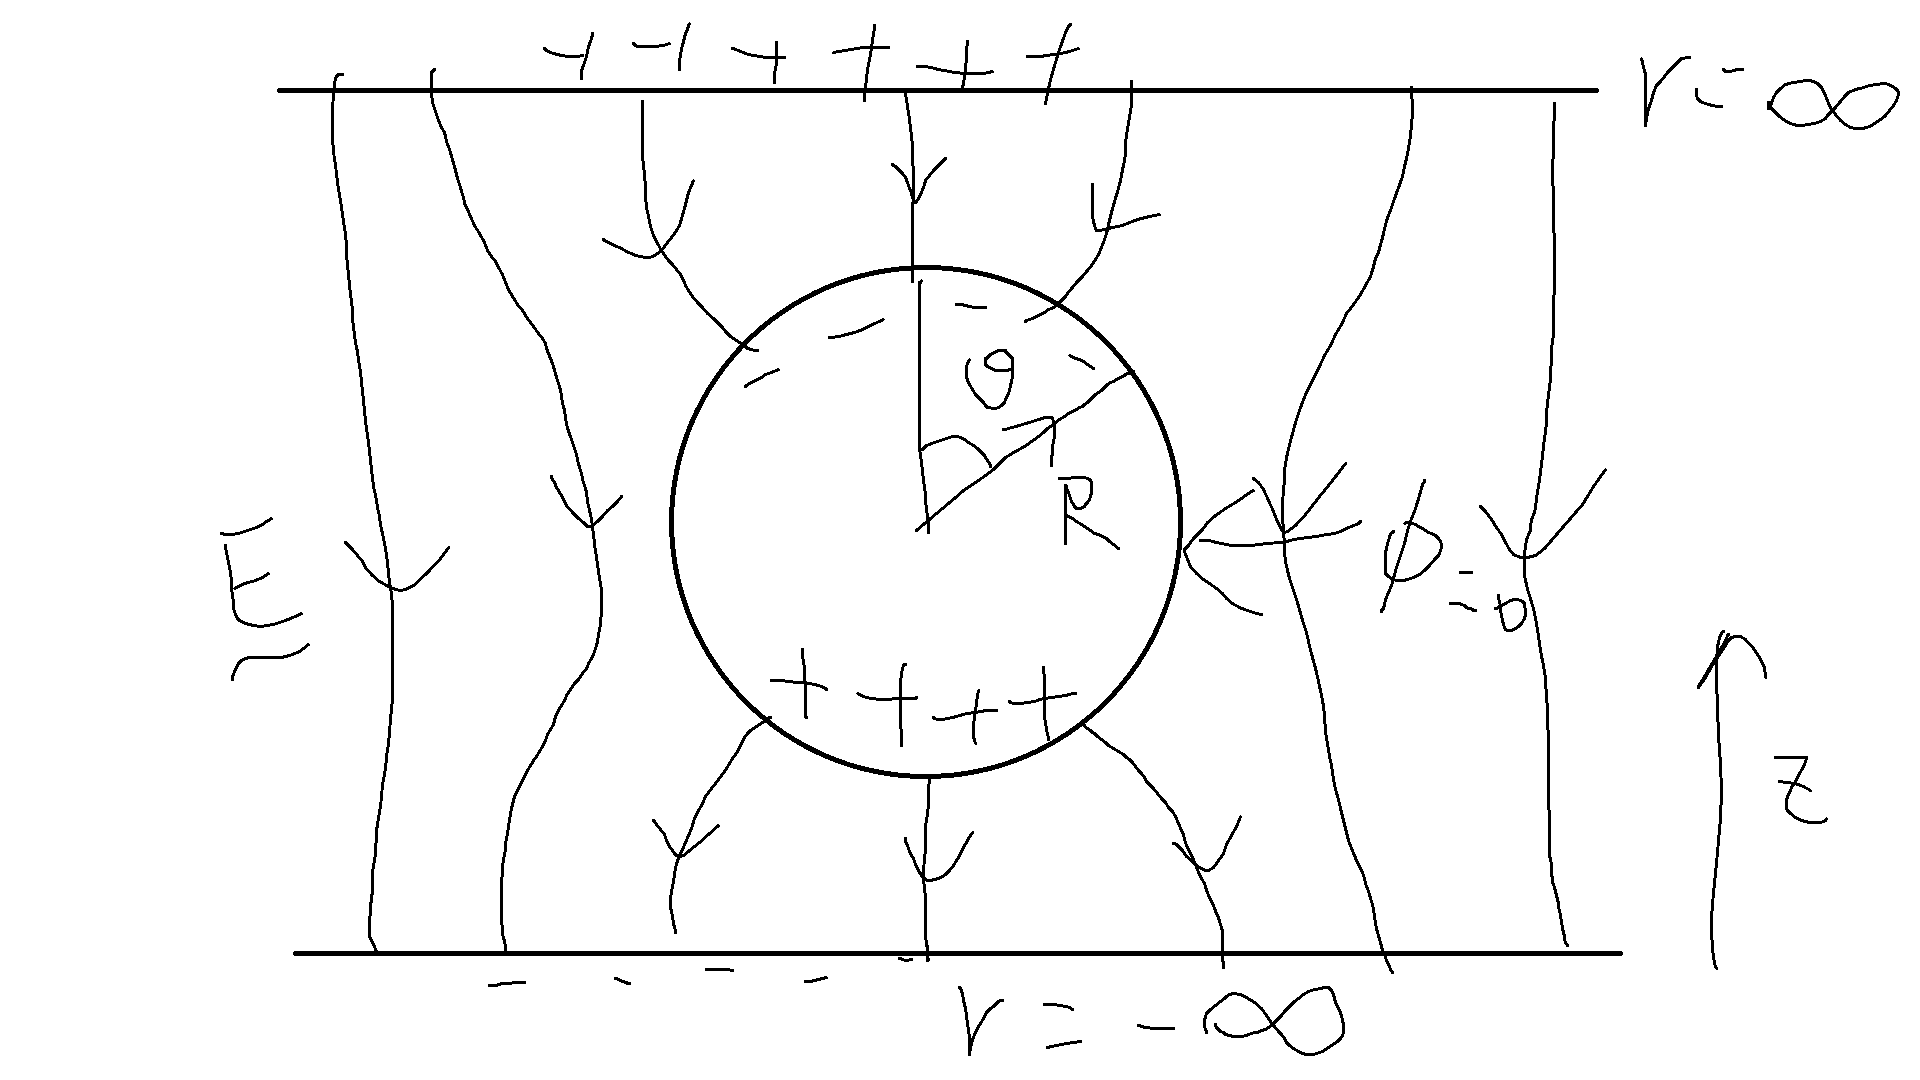
\includegraphics[scale=0.5]{EM_20}

Initially uniform field $\mathbf{E} = -E_0 \hat{\mathbf{z}}$ plus a conducting sphere (radius $S$, centre $\mathbf{r}=0$, grounded $\phi = 0$).

Cylindrical symmetry $\mathbf{E}(\mathbf{r}) = \mathbf{E}(r,\theta)$ in 3D polar coordinates.

Instead of image charge, try adding image dipole field at $\mathbf{r}=0$,
\begin{equation*}
\begin{aligned}
\phi(r,\theta) = -E_0 \hat{\mathbf{z}} + \frac{\mathbf{p} \cdot \mathbf{r}}{4\pi \varepsilon r^2}
\end{aligned}
\end{equation*}
by \eqref{eq:2.17}. By syymetry, take $\mathbf{p} = p_0 \hat{\mathbf{z}}$. So $\hat{\mathbf{r}} \cdot \hat{\mathbf{z}} = \cos \theta$.

We require $\phi=0$ at $r = |\mathbf{r}| = R$, satisfied if
\begin{equation*}
\begin{aligned}
\phi(R,\theta) = -E_0 R\cos\theta + \frac{p\cos\theta}{4\pi \varepsilon_0 R^2} = 0
\end{aligned}
\end{equation*}
So 
\begin{equation*}
\begin{aligned}
p = 4\pi\varepsilon_0 R^3 E_0
\end{aligned}
\end{equation*}
Solution for $r>R$ (by uniqueness) is
\begin{equation*}
\begin{aligned}
\phi(r,\theta) = -E_0 r \cos\theta + \frac{E_0 R^3 \cos\theta}{r^2}
\end{aligned}
\end{equation*}
the first term is a uniform field, while the second term is a dipole field.
\end{eg}

\textbf{Exercise.} Find $\mathbf{E} = -\nabla \phi$.

\subsection{Capacitors}
These are usually closely spaced conductors which store electrical energy. A potential difference $V$ caused by opposite charges $\pm Q$ accumulating, with capacitance defined by
\begin{equation*}\tag{2.32} \label{eq:2.32}
\begin{aligned}
C=\frac{Q}{V}
\end{aligned}
\end{equation*}

Consider two parallel conductor plates with area $A$, charges $\pm Q$, positined at $z=0,d$ (with $d \ll \sqrt{A}$).

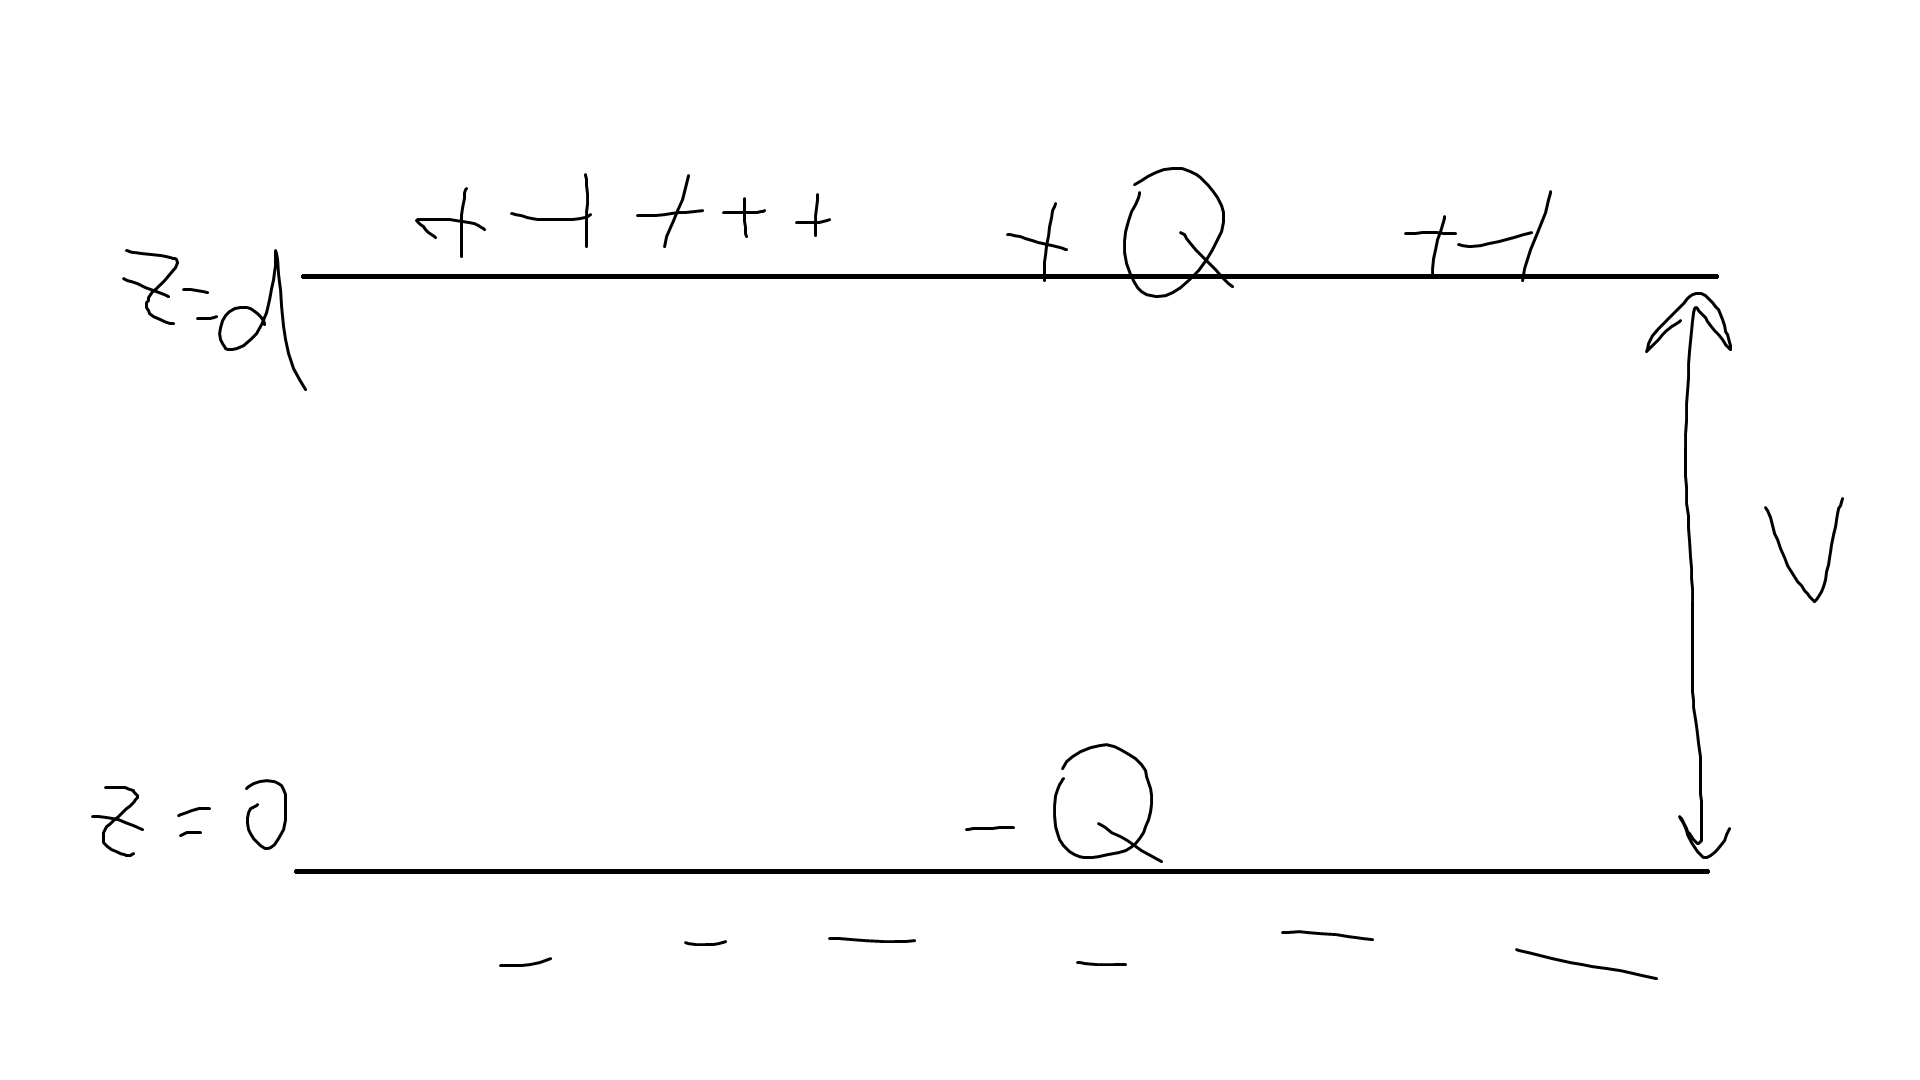
\includegraphics[scale=0.4]{EM_21}

$\mathbf{E} = -E_0 \hat{\mathbf{z}} = -\frac{\sigma}{\varepsilon_0} \hat{\mathbf{z}}$ is a constant with $\sigma = Q/A$.

Since $\mathbf{E} = -\frac{d\phi}{dz}$, we must have $\phi(z) = E_0 z + c$, and potential difference $V = \phi(d) - \phi(0) = E_0 d = \frac{Qd}{A\varepsilon_0}$.

Hence, the capacitance is
\begin{equation*}\tag{2.33} \label{eq:2.33}
\begin{aligned}
C=\frac{A\varepsilon_0}{d}
\end{aligned}
\end{equation*}

The electrical energy \eqref{eq:2.27} stored by a capacitor is
\begin{equation*}
\begin{aligned}
U=\frac{1}{2} \int d^3 \mathbf{x} \mathbf{E} \cdot \mathbf{E} = \frac{\varepsilon}{2} Ad \left(\frac{Q}{A\varepsilon_0}\right)^2 = \frac{Q^2d}{A\varepsilon} = Q^2 C  \  (\frac{Q^2}{2C}??)
\end{aligned}
\end{equation*}
by \eqref{eq:2.33}.

\textbf{Exercise.} Spherical capacitor with $\pm Q$ at $R_1 < R_2$ with
\begin{equation*}
\begin{aligned}
\phi = \frac{Q}{4\pi\varepsilon_0 r}
\end{aligned}
\end{equation*}
for $R_1<r<R_2$. Show that
\begin{equation*}
\begin{aligned}
C = \frac{4\pi\varepsilon_0 R_1 R_2}{R_2-R_1}
\end{aligned}
\end{equation*}

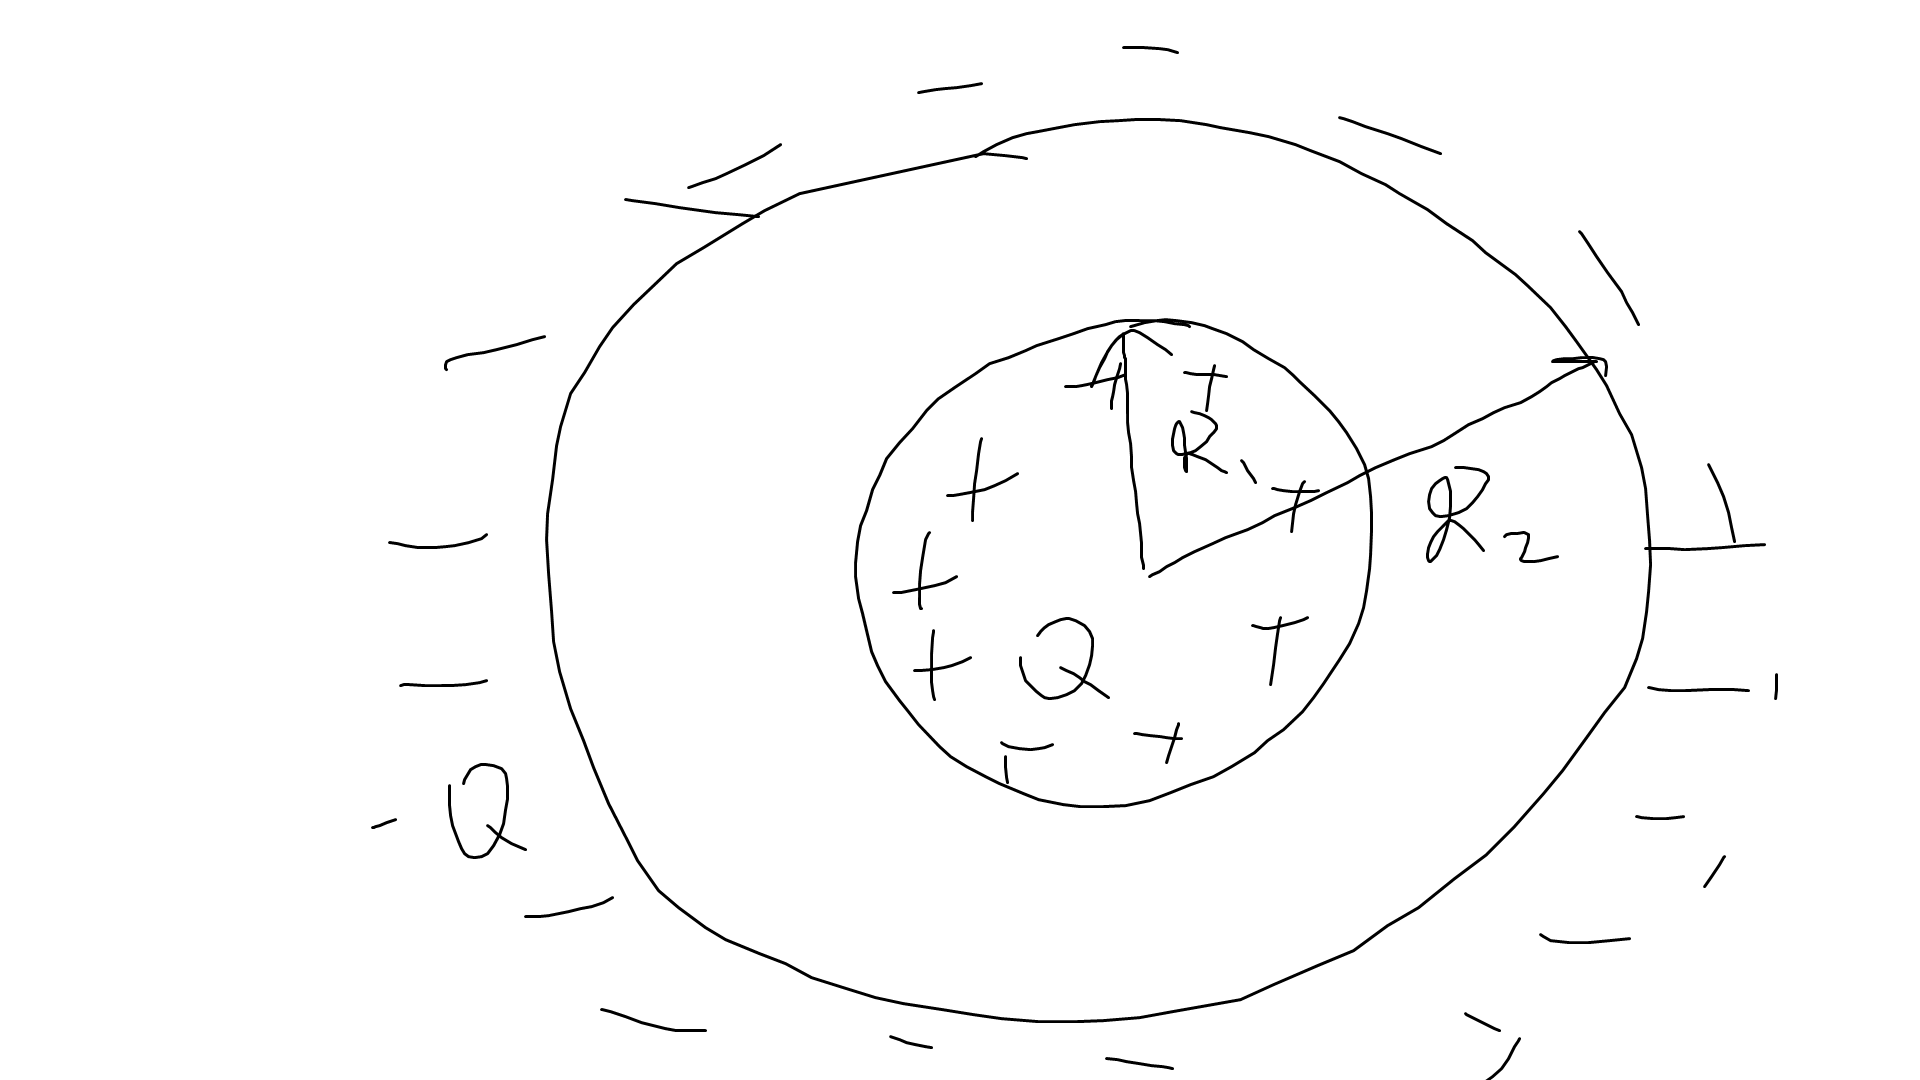
\includegraphics[scale=0.4]{EM_22}

\newpage

\section{Magnetostatics}
We will now solve Maxwell's equations sourced by steady currents $J \neq 0$ which gives rise to magnetic fields $\mathbf{B}$. We will take $\rho = 0$, $\mathbf{E} = 0$, and $\frac{\partial \mathbf{J}}{\partial t} = 0$, so \eqref{eq:1.12} - \eqref{eq:1.15} become
\begin{equation*}\tag{3.1} \label{eq:3.1}
\begin{aligned}
\nabla \times \mathbf{B} = \mu_0 J
\end{aligned}
\end{equation*}
\begin{equation*}\tag{3.2} \label{eq:3.2}
\begin{aligned}
\nabla \cdot \mathbf{B} = 0
\end{aligned}
\end{equation*}

The continuity equation \eqref{eq:1.11}, $\frac{\partial \rho}{\partial t} + \nabla \cdot \mathbf{J} = 0$ implies that
\begin{equation*}\tag{3.3} \label{eq:3.3}
\begin{aligned}
\nabla \cdot \mathbf{J} = 0
\end{aligned}
\end{equation*}

\subsection{Ampere's Law}

\subsubsection{Straight wire with steady current}
Suppose we have a steady current flowing through a surface $S$ with boundary curve $C$, element $d\mathbf{l}$. 

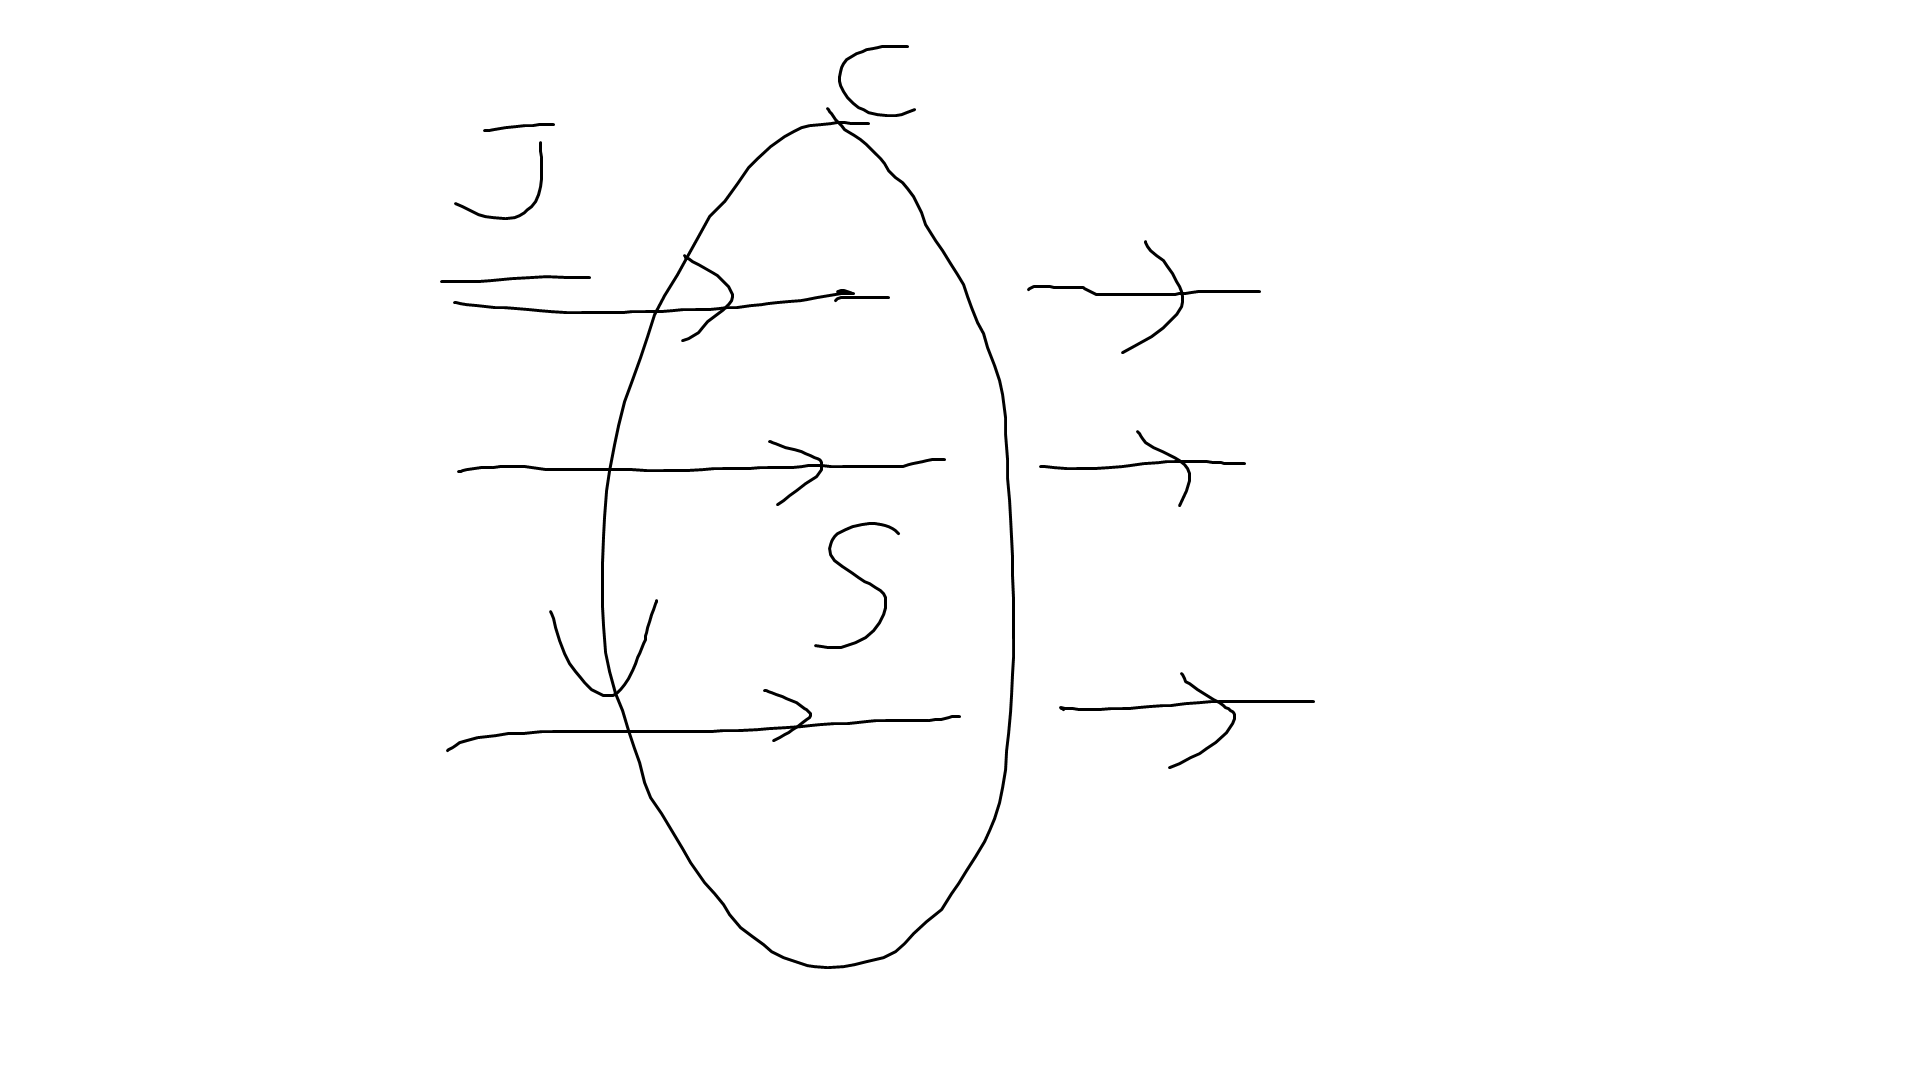
\includegraphics[scale=0.4]{EM_23}

By Stokes' theorem,
\begin{equation*}
\begin{aligned}
\int_S \nabla \times \mathbf{B} \cdot dS &= \oint_C \mathbf{B} \cdot d\mathbf{l}\\
&= \mu_0 \int \mathbf{J} \cdot d\mathbf{S}
\end{aligned}
\end{equation*}

This is Ampere's Law
\begin{equation*}\tag{3.4} \label{eq:3.4}
\begin{aligned}
\oint \mathbf{B} \cdot d\mathbf{l} = \mu_0 I
\end{aligned}
\end{equation*}
where $I$ is the current through $S$.

Consider cylindrical coordinates $(r,\varphi,z)$ with wire along $z-$axis and current $I$. By symmetry, we have $\mathbf{B}(\mathbf{r}) = B(r) \hat{\mathbf{\phi}}$. This is the \emph{right hand rule} - thumb points along current, fingers around $B$ field lines. 

Check \eqref{eq:3.2}:
\begin{equation*}
\begin{aligned}
\nabla \cdot \mathbf{B} = \frac{1}{r}\frac{\partial B(r)}{\partial \varphi} = 0
\end{aligned}
\end{equation*}

Around $z=$constant circle, we have
\begin{equation*}
\begin{aligned}
\oint \mathbf{B} \cdot d\mathbf{l} = \int_0^{2\pi} B(r) rd\varphi = 2\pi r B(r) = \mu_0 I
\end{aligned}
\end{equation*}
by Ampere's Law. So we have
\begin{equation*}\tag{3.5} \label{eq:3.5}
\begin{aligned}
B(r) = \frac{\mu_0 I}{2\pi r} \hat{\mathbf{\varphi}}
\end{aligned}
\end{equation*}
Compare with line charge \eqref{eq:2.6}.

\subsubsection{Surface currents and matching conditions}
Suppose $z=0$ plane has a steady current with current density $\mathbf{K} = k\hat{\mathbf{x}}$ (current per unit length).

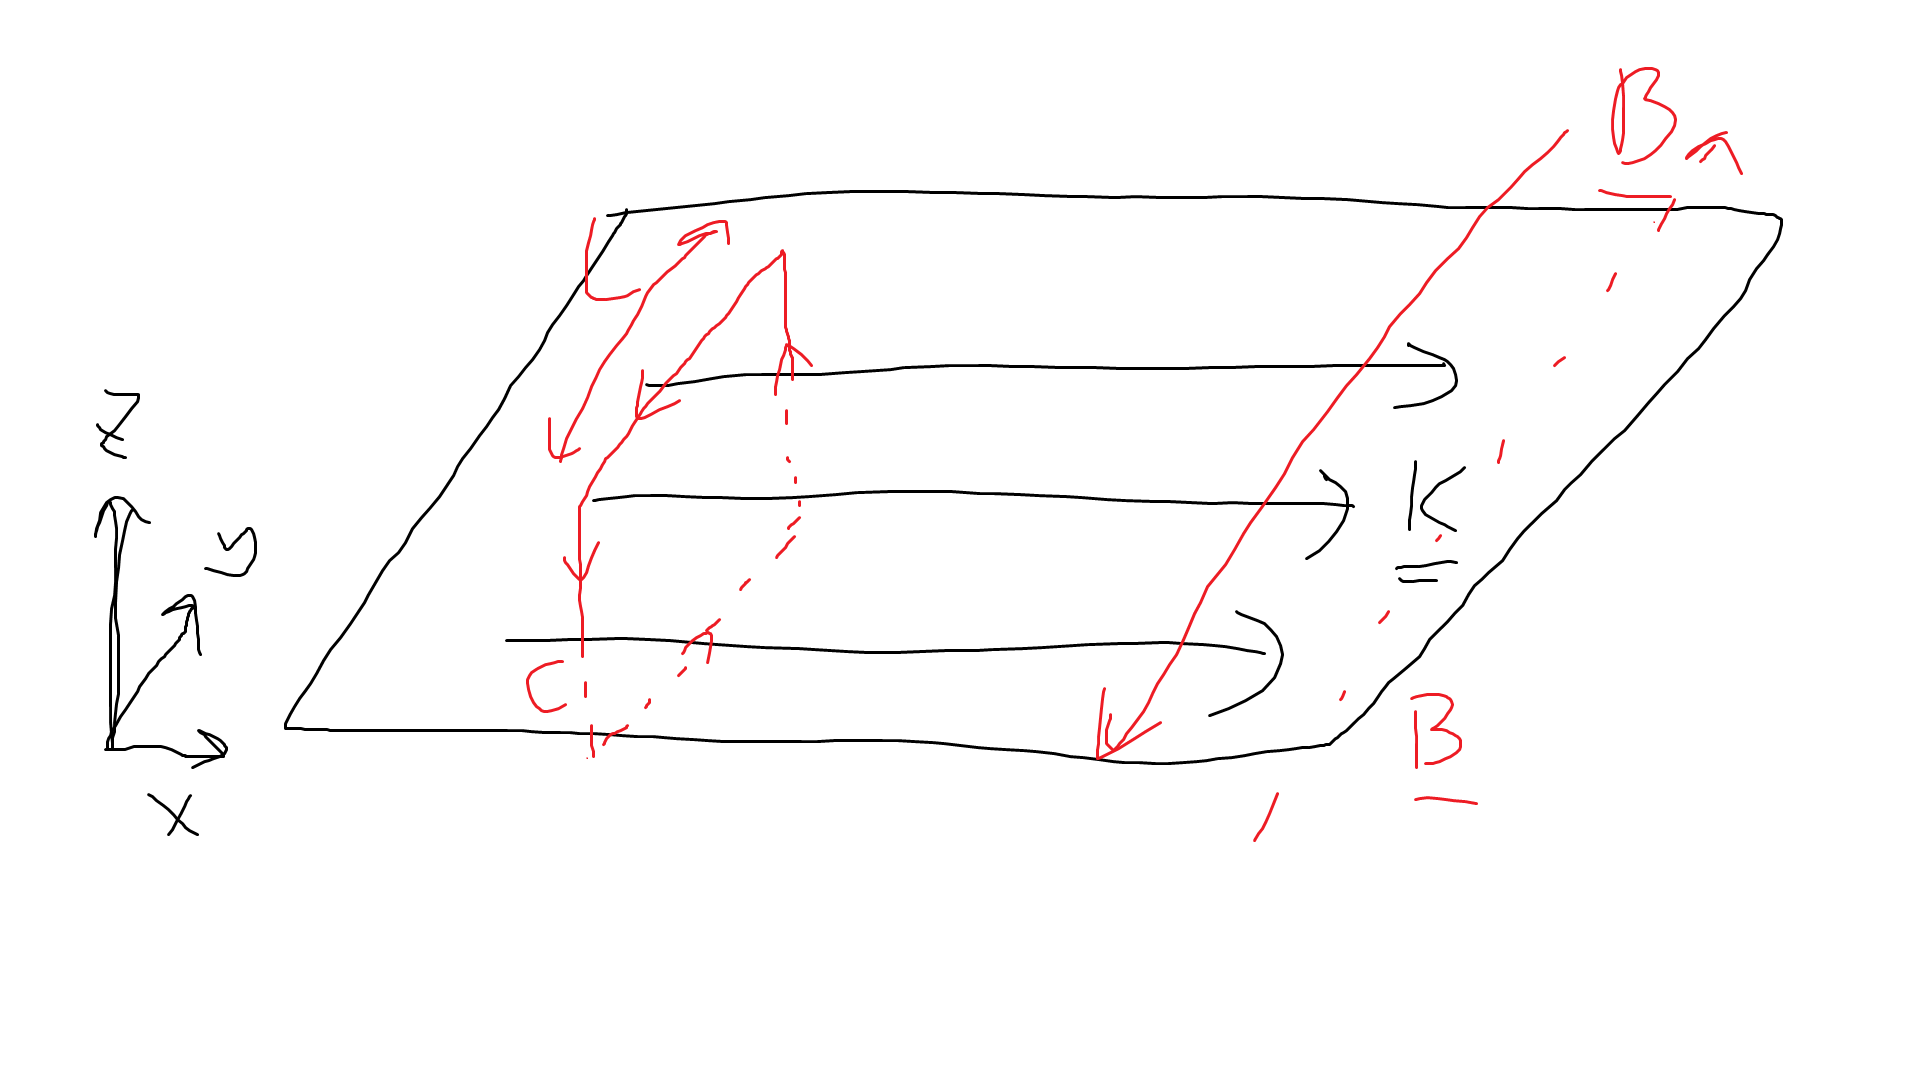
\includegraphics[scale=0.5]{EM_24}

By symmetry,
\begin{equation*}
\begin{aligned}
\mathbf{B} = \left\{\begin{array}{ll}
-B(z) \hat{\mathbf{y}} & z>0\\
B(-z) \hat{\mathbf{y}} & z<0
\end{array}\right.
\end{aligned}
\end{equation*}
Now integrate about loop of length $L$ in the $x=$constant plane, we have
\begin{equation*}
\begin{aligned}
\oint \mathbf{B} \cdot d\mathbf{l} &= LB(z) - LB(-z)\\
&= 2LB(z)\\
&= \mu_0 kL
\end{aligned}
\end{equation*}
So we have
\begin{equation*} \tag{3.6} \label{eq:3.6}
\begin{aligned}
B(z) = \frac{mu_0 k}{2}
\end{aligned}
\end{equation*}
which is a constant field (compare with \eqref{eq:2.7}).

Note the discontinuity across the surface $B(z \to 0^+) - B(z \to 0^-) = \mu_0 k$.

This can be generalized to the following matching conditions
\begin{equation*}\tag{3.7} \label{eq:3.7}
\begin{aligned}
\hat{\mathbf{n}} \times [\mathbf{B}^+ - \mathbf{B}^- ] = \mu_0 k
\end{aligned}
\end{equation*}
and
\begin{equation*}\tag{3.8} \label{eq:3.8}
\begin{aligned}
\hat{\mathbf{n}} \cdot [\mathbf{B}^+ - \mathbf{B}^- ] = 0
\end{aligned}
\end{equation*}
Note the duality with $\mathbf{E}$, see \eqref{eq:2.8} -\eqref{eq:2.9}.

\subsubsection{Solenoid}

By wrapping wire continuously around a cylinder, we can create a circular surface current (infinite length).

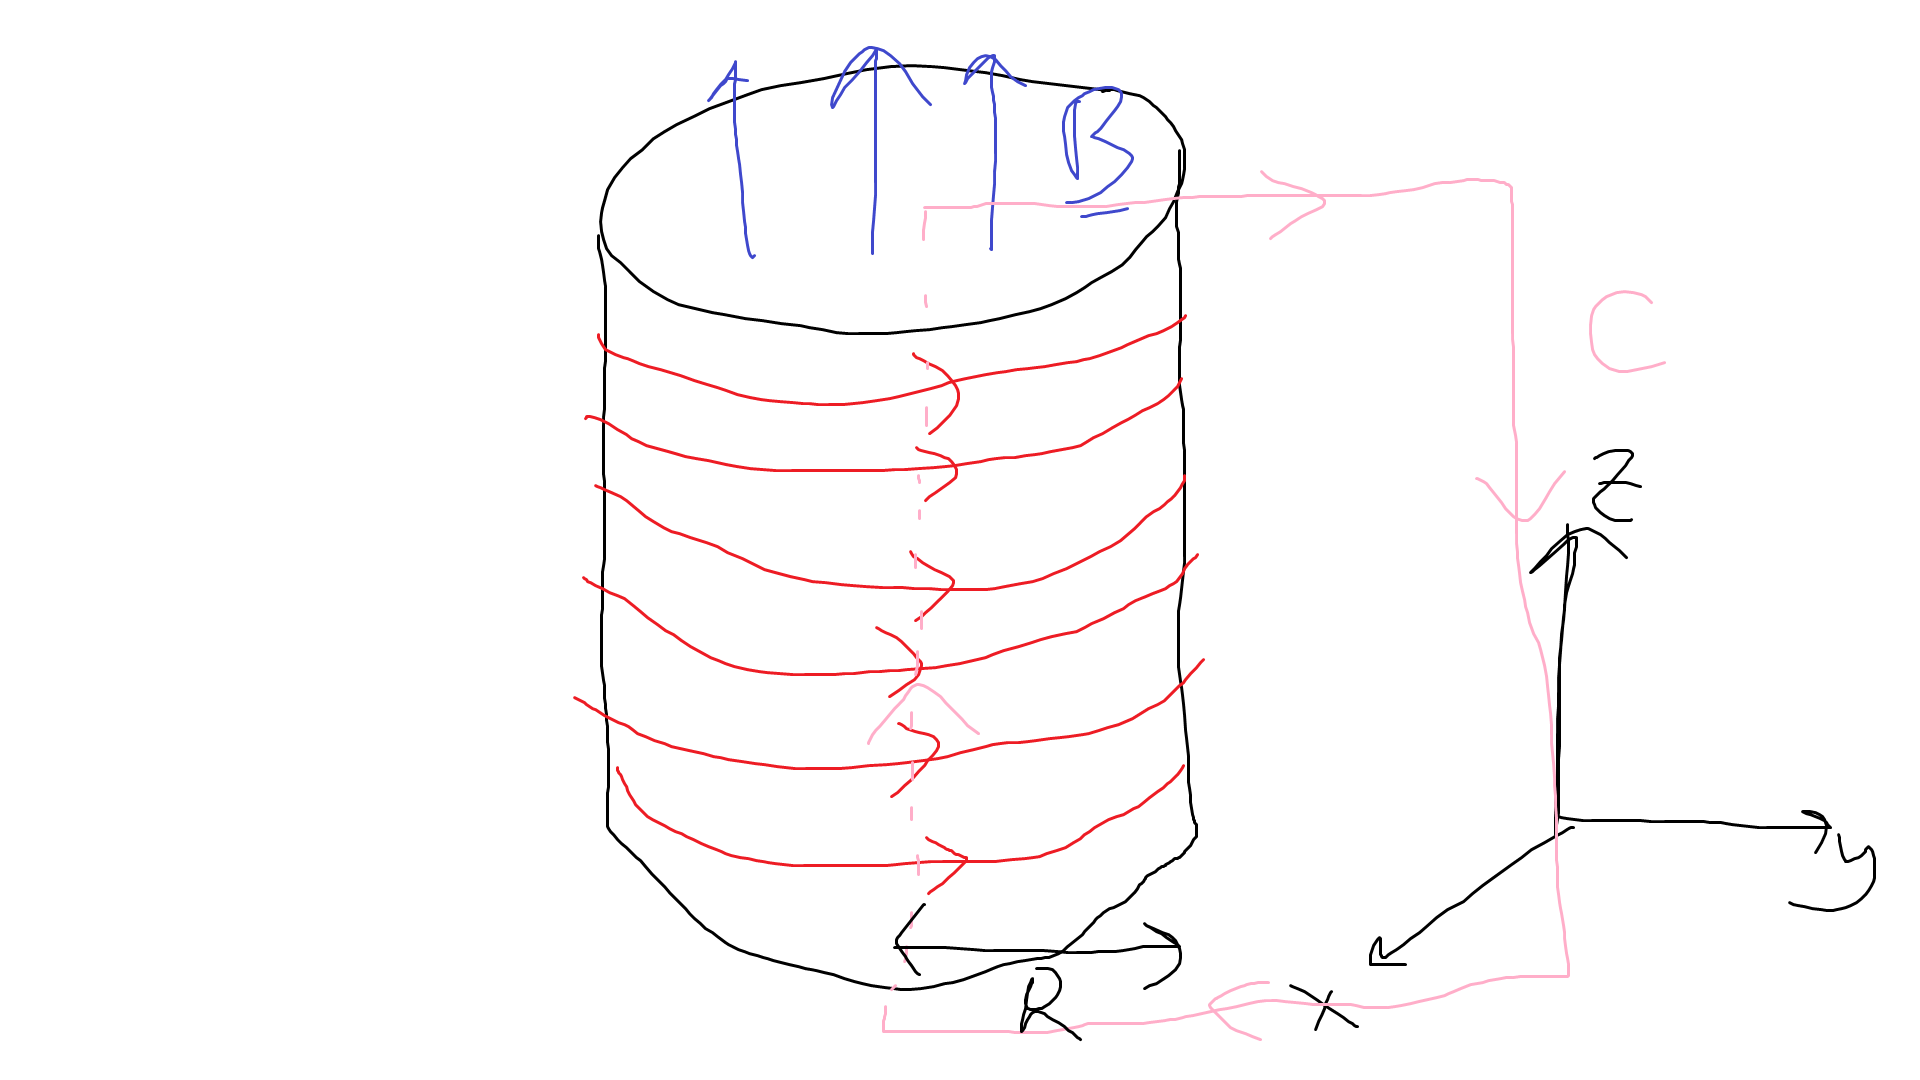
\includegraphics[scale=0.4]{EM_25}

By symmetry, $\mathbf{B} = b(r) \hat{\mathbf{z}}$ with $r=\sqrt{x^2+y^2}$.

Away from surface $\mathbf{J} = 0$, so by \eqref{eq:3.1}, $\nabla \times \mathbf{B} = 0$, so $\frac{dB}{dr} = 0 \implies B(r)=$constant.

Consider the curve $C$: Outside $r>R$ we must have $B \equiv 0$, since physically $B \to 0$ as $r \to \infty$. Apply Ampere's law,
\begin{equation*}
\begin{aligned}
\int \mathbf{B} \cdot d\mathbf{l} &= BL + 0 + 0 + 0 = BL\\
&= \mu_0 I NL
\end{aligned}
\end{equation*}
where $I$ is the current in each wire the $N$ is the number of winding per unit length. So we have
\begin{equation*}\tag{3.9} \label{eq:3.9}
\begin{aligned}
B = \mu_0 I N.
\end{aligned}
\end{equation*}

Check \eqref{eq:3.7}:
\begin{equation*}
\begin{aligned}
B= \left\{\begin{array}{ll}
\mu_0 IN \hat{\mathbf{z}} & r<R\\
0 & r>R
\end{array}\right.
\end{aligned}
\end{equation*}
So $\hat{\mathbf{n}} \times \Delta \mathbf{B} = \mu_0 \mathbf{K}$, where $\mathbf{K} = IN \hat{\mathbf{z}}$ which is consistent.

\subsection{Vector potential}
Recall from Methods the \emph{Helmholtz theorem}, that any vector field $\mathbf{F}$ can be decomposed as 
\begin{equation*}\tag{3.10} \label{eq:3.10}
\begin{aligned}
\mathbf{F} = \nabla \phi + \nabla \times \mathbf{A}
\end{aligned}
\end{equation*}
i.e. a curl-free (irrotational) part and a divergence-free (solenoidal) part, where $\mathbf{F} \to 0$ as $r \to \infty$,
\begin{equation*}
\begin{aligned}
\phi(\mathbf{r}) = \frac{1}{4\pi} \int \frac{\nabla_\mathbf{r} \cdot \mathbf{F}(\mathbf{r}')}{|\mathbf{r} - \mathbf{r}'|} d^3 \mathbf{r}'
\end{aligned}
\end{equation*}
and
\begin{equation*}
\begin{aligned}
\mathbf{A}(\mathbf{r}) = \frac{1}{4\pi} \int \frac{\nabla_\mathbf{r'} \times \mathbf{F}(\mathbf{r'})}{|\mathbf{r}-\mathbf{r'}|} d^3 \mathbf{r}'.
\end{aligned}
\end{equation*}

For magnetostatics $\nabla \times \mathbf{B} = 0$, we can describe it with a vector potential $\mathbf{A}$,
\begin{equation*}\tag{3.11} \label{eq:3.11}
\begin{aligned}
\mathbf{B} = \nabla \times \mathbf{A}
\end{aligned}
\end{equation*}
Now applies \eqref{eq:3.1},
\begin{equation*}
\begin{aligned}
\nabla \times \mathbf{B} = \nabla \times (\nabla \times \mathbf{A}) = -\nabla^2 \mathbf{A} + \nabla(\nabla \cdot \mathbf{A})
\end{aligned}
\end{equation*}
so
\begin{equation*}\tag{3.12} \label{eq:3.12}
\begin{aligned}
-\nabla^2 \mathbf{A} + \nabla(\nabla \cdot \mathbf{A}) = \mu_0 \mathbf{J}.
\end{aligned}
\end{equation*}

\subsubsection{Gauge transformations}
Note that $\mathbf{B}$ is unique, but $\mathbf{A}$ is not. Consider
\begin{equation*}\tag{3.13} \label{eq:3.13}
\begin{aligned}
\mathbf{A}'(\mathbf{r}) = \mathbf{A}(\mathbf{r}) + \nabla \chi(\mathbf{r})
\end{aligned}
\end{equation*}
for some arbitrary smooth function $\chi$.

Clearly $\nabla \times \mathbf{A}' = \nabla \times \mathbf{A}$.

\subsubsection{Coulomb gauge}
It is \emph{often} convenient to choose $\chi$ s.t. $\nabla \cdot \mathbf{A}' = 0$.e In other words, we fix to the Coulomb gauge. Can we always do this?

Consider gauge transformation $\mathbf{A}' = \mathbf{A} + \nabla x$ yielding identical $\mathbf{B} = \nabla \times \mathbf{A}$. Suppose $\nabla \cdot \mathbf{A} = \psi(\mathbf{r}) \neq 0$, then
\begin{equation*}
\begin{aligned}
\nabla \cdot \mathbf{A'} = \nabla \cdot \mathbf{A} + \nabla^2 \xi = \psi (\mathbf{r}) + \nabla^2 \xi = 0
\end{aligned}
\end{equation*}
if $\xi$ satisfies Poisson's equation $\nabla^2 \psi = \psi(x)$ for which there is always a unique solution.

\textbf{Exercise} For the straight wire \eqref{eq:3.5}, verify that
\begin{equation*}
\begin{aligned}
\mathbf{A}(\mathbf{r}) = \frac{-\mu_0 I}{2\pi} \ln r \hat{\mathbf{z}}
\end{aligned}
\end{equation*}
and reproduces the correct magnetic field
\begin{equation*}
\begin{aligned}
\mathbf{B}(\mathbf{r}) = \frac{\mu_0 I}{2\pi r} \hat{\mathbf{\varphi}} = \frac{\mu_0I}{2\pi r} \left(-\frac{y}{r} \hat{\mathbf{x}} + \frac{x}{y}\hat{\mathbf{y}}\right)
\end{aligned}
\end{equation*}
(and is in the Coulomb gauge $\nabla \cdot \mathbf{A} = 0$).

\subsection{Biot-Savart Law}
Consider \eqref{eq:3.12} in Coulomb gauge $\nabla \cdot \mathbf{A} = 0$, so Maxwell equation \eqref{eq:3.1} becomes
\begin{equation*}
\begin{aligned}
\nabla \times \mathbf{B} = \nabla \times (\nabla \times \mathbf{A}) = -\nabla^2 \mathbf{A} + \nabla(\nabla\cdot \mathbf{A}) = \mu_0 \mathbf{J}
\end{aligned}
\end{equation*}
So
\begin{equation*}\tag{3.16} \label{eq:3.16}
\begin{aligned}
\nabla^2 \mathbf{A} = \mu_0 \mathbf{J}
\end{aligned}
\end{equation*}
or in components, for $i=1,2,3$
\begin{equation*}
\begin{aligned}
\nabla^2 A_i = -\mu_0 J_i
\end{aligned}
\end{equation*}
which are 3 copies of Poisson equations. We've solve this already with Green's functions \eqref{eq:2.20}, implying
\begin{equation*}
\begin{aligned}
A_i(\mathbf{x}) = \frac{\mu_0}{4\pi} \int_V d^3 \mathbf{x}' \frac{J_i(\mathbf{x}')}{|\mathbf{x}-\mathbf{x}'|}
\end{aligned}
\end{equation*}
or
\begin{equation*}\tag{3.17} \label{eq:3.17}
\begin{aligned}
\mathbf{A}(\mathbf{x}) = \frac{\mu_0}{4\pi} \int_V d^3 \mathbf{x}' \frac{\mathbf{J}(\mathbf{x}')}{|\mathbf{x}-\mathbf{x}'|}
\end{aligned}
\end{equation*}
The magnetic field is then (using $\nabla \times (\psi \mathbf{D}) = \psi \nabla \times \mathbf{D} + \nabla \psi \times \mathbf{D}$),
\begin{equation*}
\begin{aligned}
\mathbf{B}(\mathbf{x}) = \nabla \times \mathbf{A}(\mathbf{x}) &= \frac{\mu_0}{4\pi} \int_V d^3 \mathbf{x}' \nabla_\mathbf{x} \times \left( \frac{\mathbf{J}(\mathbf{x})}{|\mathbf{x}-\mathbf{x}'|} \right)\\
&= \frac{\mu_0}{4\pi} \int d^3 \mathbf{x}' \left[\frac{\nabla_\mathbf{x} \times \mathbf{J}(\mathbf{x}')}{|\mathbf{x}-\mathbf{x}'|} + \nabla_\mathbf{x} \left(\frac{1}{|\mathbf{x}-\mathbf{x}'|} \right) \times \mathbf{J} (\mathbf{x}')\right]
\end{aligned}
\end{equation*}
The first term is $0$ as there is no $\mathbf{x}-$dependence, and the second term is equal to $\frac{-(\mathbf{x}-\mathbf{x}')}{|\mathbf{x}-\mathbf{x}'|^3}$. Hence, we have \emph{Biot-Savart Law},
\begin{equation*}\tag{3.18} \label{eq:3.18}
\begin{aligned}
\mathbf{B}(\mathbf{x}) = \frac{\mu_0}{4\pi} \int d^3 \mathbf{x}' \frac{\mathbf{J}(\mathbf{x}') \times (\mathbf{x}-\mathbf{x}')}{|\mathbf{x}-\mathbf{x}'|^3}
\end{aligned}
\end{equation*}
For localized current along a curve $C$ (by straight wire with $\mathbf{J}(\mathbf{x}) = I\delta(x) \delta(y) \hat{\mathbf{z}}$), then \eqref{eq:3.18} becomes
\begin{equation*}\tag{3.19} \label{eq:3.19}
\begin{aligned}
\mathbf{B}(\mathbf{x}) = \frac{\mu_0 I}{4\pi} \oint_C \frac{d\mathbf{x}' \times (\mathbf{x}-\mathbf{x}')}{|\mathbf{x}-\mathbf{x}'|^3}
\end{aligned}
\end{equation*}

Aside: verify $\mathbf{A}(\mathbf{x})$ in \eqref{eq:3.17} is in Coulomb gauge $\nabla \cdot \mathbf{A} = 0$:
\begin{equation*}
\begin{aligned}
\nabla_\mathbf{x}\cdot \mathbf{A}(\mathbf{x}) &= \frac{\mu_0}{4\pi} \int_V d^3 \mathbf{x}' \mathbf{J}(\mathbf{x}') \cdot \nabla_\mathbf{x} \left(\frac{1}{|\mathbf{x}-\mathbf{x}'|} \right)\\
&= \frac{-\mu_0}{4\pi} \int d^3 \mathbf{x}' \mathbf{J}(\mathbf{x}') \cdot \nabla_\mathbf{x'} \left(\frac{1}{|\mathbf{x}-\mathbf{x}'|}\right)\\
\end{aligned}
\end{equation*}
since if we interchange $\mathbf{x} \leftrightarrow \mathbf{x}'$, 
\begin{equation*}
\begin{aligned}
\nabla_\mathbf{x} \left(\frac{1}{|\mathbf{x}-\mathbf{x}'|}\right) = -\nabla_\mathbf{x'} \left(\frac{1}{|\mathbf{x}-\mathbf{x}'|}\right)
\end{aligned}
\end{equation*}
and the above then equals
\begin{equation*}
\begin{aligned}
\frac{-\mu_0}{4\pi} \int_V d^3 \mathbf{x}' \left[\nabla_\mathbf{x'} \left(\frac{\mathbf{J}(\mathbf{x'})}{|\mathbf{x}-\mathbf{x}'|}\right) - \frac{\nabla_\mathbf{x'} \cdot \mathbf{J}(\mathbf{x}')}{|\mathbf{x}-\mathbf{x}'|}\right] =0 
\end{aligned}
\end{equation*}
by \eqref{eq:3.3} the continuity equation.

\subsection{Current loop and magnetic dipole}
Consider a circular loop, current $I$, radius $R$, lying in $z=0$ plane. We could solve \eqref{eq:3.17} directly with $$\mathbf{J} = I\sin\theta \delta(\cos\theta) \frac{\delta(r-R)}{R} \times (-\sin\varphi \hat{\mathbf{i}} + \cos\varphi\hat{\mathbf{j}})$$ but we will seek a far-field ($|\mathbf{r}| \gg |\mathbf{r}'|| = R$) solution only.

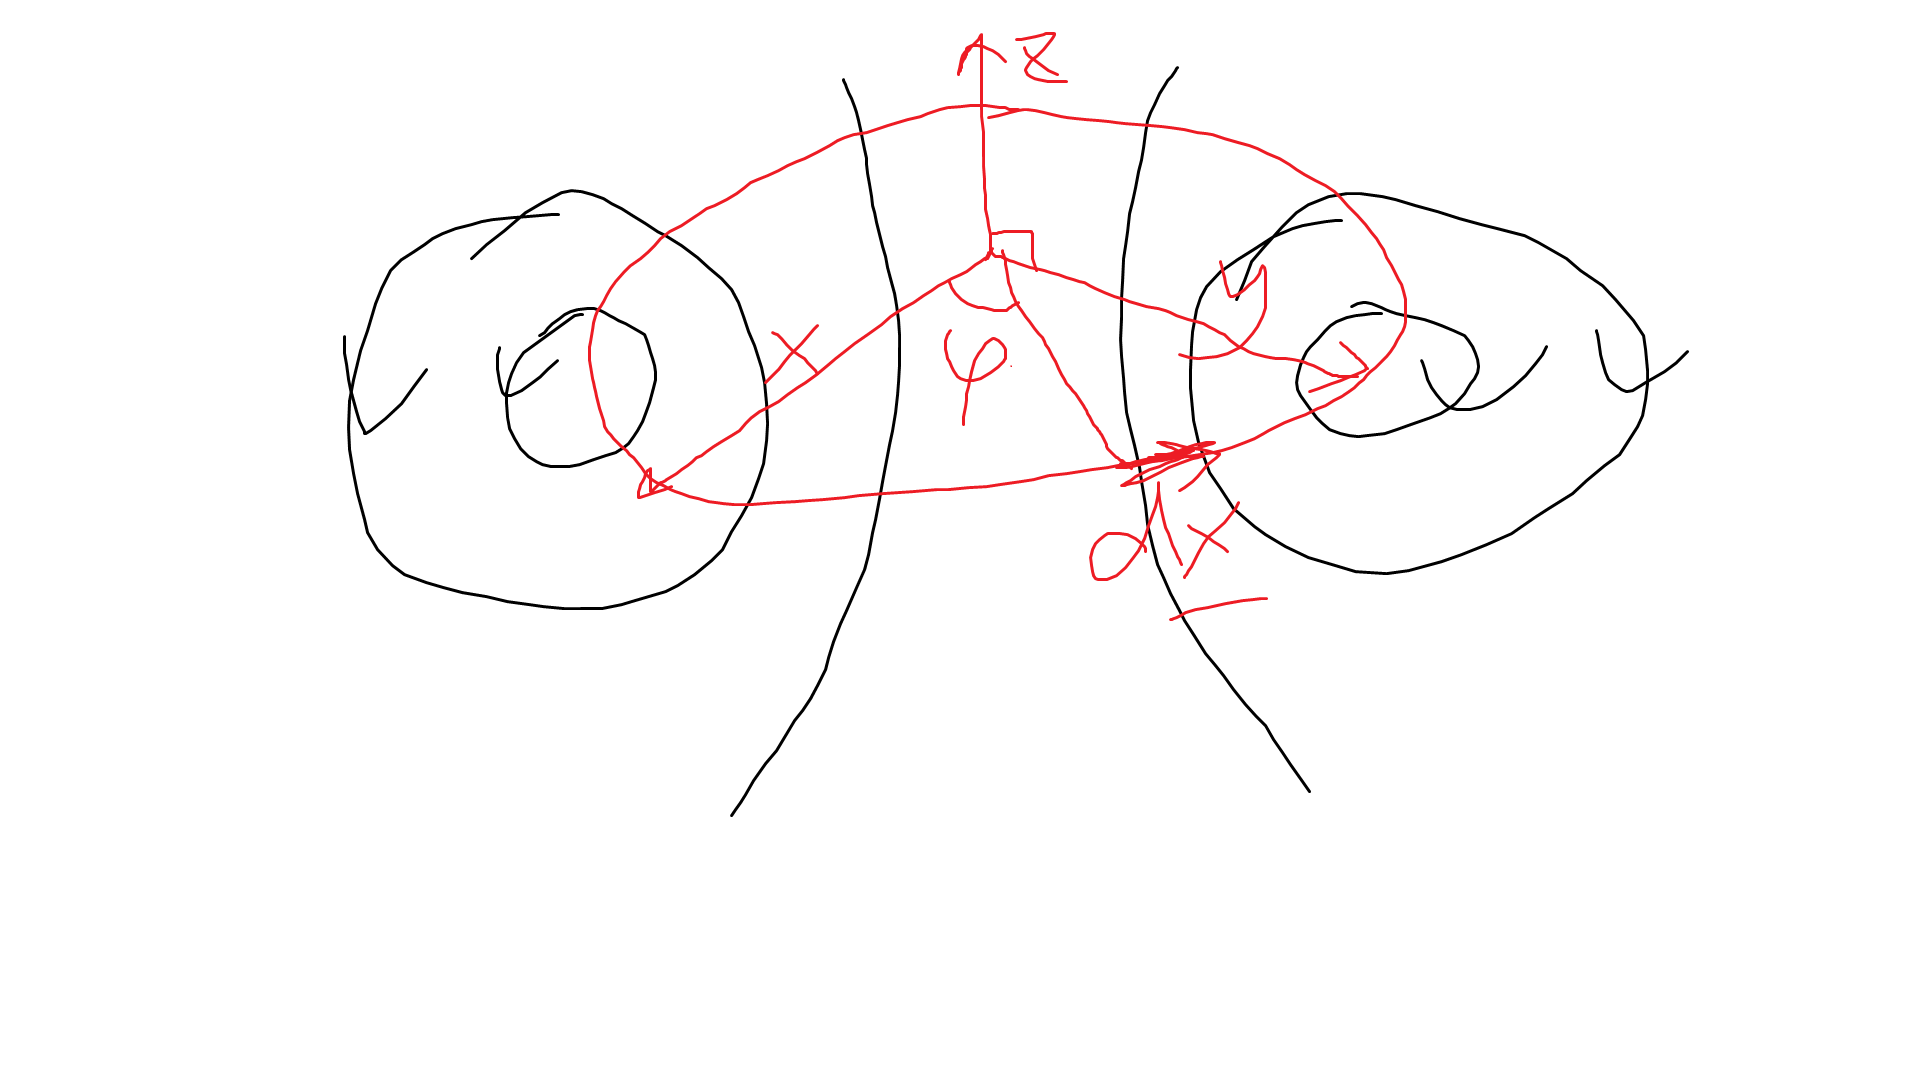
\includegraphics[scale=0.5]{EM_26}

The vector potential $\mathbf{A}(\mathbf{x})$ \eqref{eq:3.17} expands as
\begin{equation*}\tag{3.20} \label{eq:3.20}
\begin{aligned}
\mathbf{A}(\mathbf{r}) &= \frac{\mu_0I}{4\pi} \oint \frac{dr'}{|\mathbf{r}-\mathbf{r}'|}\\
&= \frac{\mu_0}{4\pi} \oint d\mathbf{r}' \left(\frac{1}{r} + \frac{\mathbf{r} \cdot \mathbf{r}'}{r^3} + ... \right) 
\end{aligned}
\end{equation*}
under localized current. Also the integral involving $\frac{1}{r}$ vanishes around the loop. So
\begin{equation*}
\begin{aligned}
\mathbf{A}(\mathbf{r}) = \frac{\mu_0I}{4\pi r^3} \oint \mathbf{r}\cdot\mathbf{r}' d\mathbf{r}' = \frac{-\mu_0I}{4\pi r^3} \int_S \nabla_{\mathbf{r}'} (\mathbf{r}\cdot\mathbf{r}')\times dS
\end{aligned}
\end{equation*}
because of Green's theorem
\begin{equation*}
\begin{aligned}
\oint_C fd\mathbf{r} = \int \nabla f \times d\mathbf{S}.
\end{aligned}
\end{equation*}
The above is then equal to
\begin{equation*}
\begin{aligned}
\frac{-\mu_0I}{4\pi r^3} \int_S \mathbf{r} \times d\mathbf{S} = \frac{\mu_0I}{4\pi r^3} \mathbf{r} \times \int d\mathbf{S}
\end{aligned}
\end{equation*}
since $\mathbf{r}$ is juts a constant vector in this integral. Now the integral of $d\mathbf{S}$ is the vector area $\mathbf{S}$ of surface $S$. So the above is equal to
\begin{equation*}
\begin{aligned}
-\frac{\mu_0I}{4\pi} \frac{\mathbf{r} \times \mathbf{S}}{r^3}
\end{aligned}
\end{equation*}
Define a \emph{magnetic dipole moment} by 
\begin{equation*}\tag{3.21} \label{eq:3.21}
\begin{aligned}
\mathbf{m} = I\mathbf{S}
\end{aligned}
\end{equation*}
and far field is
\begin{equation*}\tag{3.22} \label{eq:3.22}
\begin{aligned}
\mathbf{A}(\mathbf{r}) = \frac{\mu_0}{4\pi} \frac{\mathbf{m} \times \mathbf{r}}{r^3}.
\end{aligned}
\end{equation*}

\textbf{Exercise} Show that the magnetic dipole field $\mathbf{B}(\mathbf{r})$ takes an identical form to the electric dipole \eqref{eq:2.18}, i.e.,
\begin{equation*}\tag{3.23} \label{eq:3.23}
\begin{aligned}
\mathbf{B}(\mathbf{r}) = \nabla \times \mathbf{A}(\mathbf{r}) = \frac{\mu_0I}{4\pi} \left(\frac{3(\mathbf{m} \cdot \hat{\mathbf{r}})\hat{\mathbf{r}}-\mathbf{m}}{r^3}\right)
\end{aligned}
\end{equation*}

\subsubsection{General magnetic field solutions}
For a general current distribution $\mathbf{J}(\mathbf{x})$, note the following identities (note summation conventions)
\begin{equation*}\tag{*}
\begin{aligned}
\frac{\partial}{\partial x_i}(J_i x_j) = \frac{\partial J_i}{\partial x_i} x_j + J_i \delta_{ij} = J_j
\end{aligned}
\end{equation*}
since the first term is zero by the continuity equation $\nabla \cdot \mathbf{J}=0$. So $\mathbf{J}$ can be expressed as a total derivative
\begin{equation*}\tag{$\dagger$}
\begin{aligned}
\frac{\partial}{\partial x_i}(J_i x_j x_k) = \frac{\partial J_i}{\partial x_i} x_j x_k + J_j x_k + J_k x_j = J_j x_k + J_k x_j
\end{aligned}
\end{equation*}
So the general solution \eqref{eq:3.17} becomes
\begin{equation*}
\begin{aligned}
A_i (\mathbf{x}) = \frac{\mu_0}{4\pi} \int d^3 \mathbf{x}' \frac{J_i(\mathbf{x}')}{|\mathbf{x}-\mathbf{x}'|} &= \frac{\mu_0}{4\pi} \int d^3 \mathbf{x}' \times \left(\frac{J_i(\mathbf{x}'}{r} + \frac{J_i(\mathbf{x}' (\mathbf{x} \cdot \mathbf{x}')}{r^3}+...\right)\\
&=\frac{\mu_0}{4\pi} \left\{\frac{1}{r}\int d^3 \mathbf{x}' \frac{\partial}{\partial x_j} (J_j x'_i) + 
\frac{x_j}{r^3} \int d^3 \mathbf{x}' \left[\frac{1}{2} J_i x'_j + \frac{1}{2} J_i x'_i + \frac{1}{2} J_i x'_j - \frac{1}{2} J_i x'_i \right]\right\}
\end{aligned}
\end{equation*}
for the first term, by (*), the surface term
\begin{equation*}
\begin{aligned}
\sim \frac{1}{r}\int_S x'_i J_i dS_j = 0
\end{aligned}
\end{equation*}
vanishes with $V \subset V$ interior sources ($r' \ll r$). And for the second term, by ($\dagger$) the surface term is $\frac{1}{2} \frac{\partial}{\partial x_i} (J_k x'_i x'_j)$. So above is equal to
\begin{equation*}
\begin{aligned}
&\frac{\mu_0}{4\pi r^3} \frac{x_j}{2} \int d^3 \mathbf{x}' (J_i x'_j - J_j x'_i)\\
=& \frac{\mu_0}{4\pi r^3} \frac{1}{2} \int d^3 \mathbf{x}' \left[J_i (\mathbf{x}\cdot \mathbf{x}') - x'_i (\mathbf{J} \cdot \mathbf{x})\right]\\
&= \frac{-\mu_0}{4\pi r^3} \frac{1}{2} \left[\mathbf{x} \times \int d^3 \mathbf{x}' J(\mathbf{x}' \times \mathbf{x}'\right]
\end{aligned}
\end{equation*}
Hence 
\begin{equation*}\tag{3.24} \label{eq:3.24}
\begin{aligned}
\mathbf{A}(\mathbf{r}) = \frac{\mu_0}{4\pi} \frac{\mathbf{m} \times \mathbf{r}}{r^3}
\end{aligned}
\end{equation*}
where 
\begin{equation*}\tag{3.25} \label{eq:3.25}
\begin{aligned}
\mathbf{m} = \frac{1}{2} \int d^3\mathbf{r}' (\mathbf{r}' \times \mathbf{J}(\mathbf{r}'))
\end{aligned}
\end{equation*}

\subsection{Magnetic Forces}
Ampere showed that one current-carrying wire (current $I_1$) exerts a force on a second wire ($I_2$), so consider the force on the second wire in the $\mathbf{B}-$field of the first.

\subsubsection{Two straight wires}

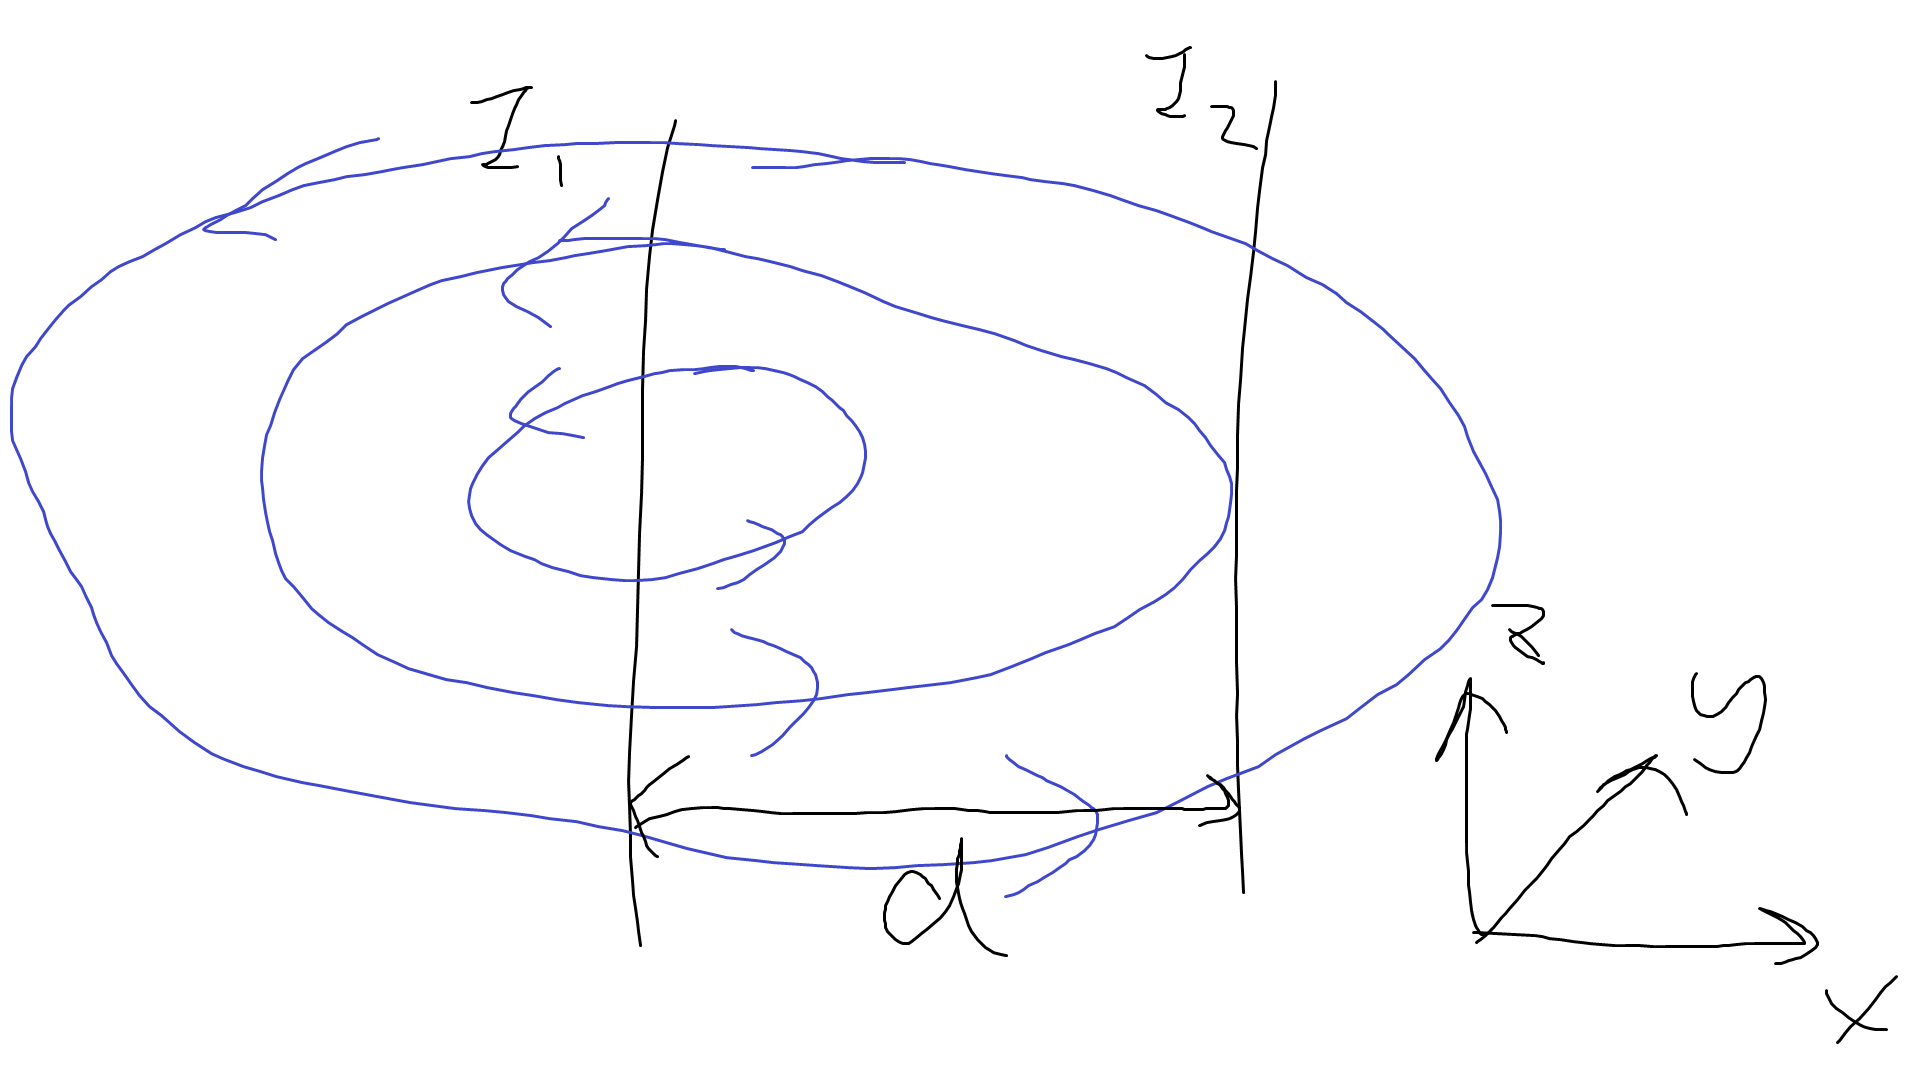
\includegraphics[scale=0.4]{EM_27}

Parallel to $z-$axis, distance $d$ apart. So we have \eqref{eq:3.5},
\begin{equation*}
\begin{aligned}
B_1 = \frac{\mu_0 I_1}{2\pi r} \hat{\mathbf{\varphi}}.
\end{aligned}
\end{equation*}
Also, $\mathbf{J}_2 = nq\mathbf{v}$, where $n$ is the density of charge carriers and $\mathbf{v}$ is the average velocity in the $z-$direction, and $I_2 = J_2 A$, where $A$ is the cross-sectional area of wire.

From the Lorentz force $\mathbf{F} = q\mathbf{v} \times \mathbf{B}$, we get a force law per unit length,
\begin{equation*}\tag{3.26} \label{eq:3.26}
\begin{aligned}
\mathbf{f} = nA \mathbf{F} = nAq\mathbf{v} \times \mathbf{B}_1 = A\mathbf{J}_2 \times \mathbf{B}_1 = \mu_0 \frac{I_1 I_2}{2\pi d} \hat{\mathbf{z}} \times \hat{\mathbf{\varphi}} = -\mu_0 \frac{I_1I_2}{2\pi d} \hat{\mathbf{x}}
\end{aligned}
\end{equation*}
where $nA$ is the number of charge carriers per unit length.

If $I_1$ and $I_2$ have the \emph{same} direction ($I_1 I_2>0$), then the force is attractive. Conversely, the force is repulsive.

\subsection{General case}

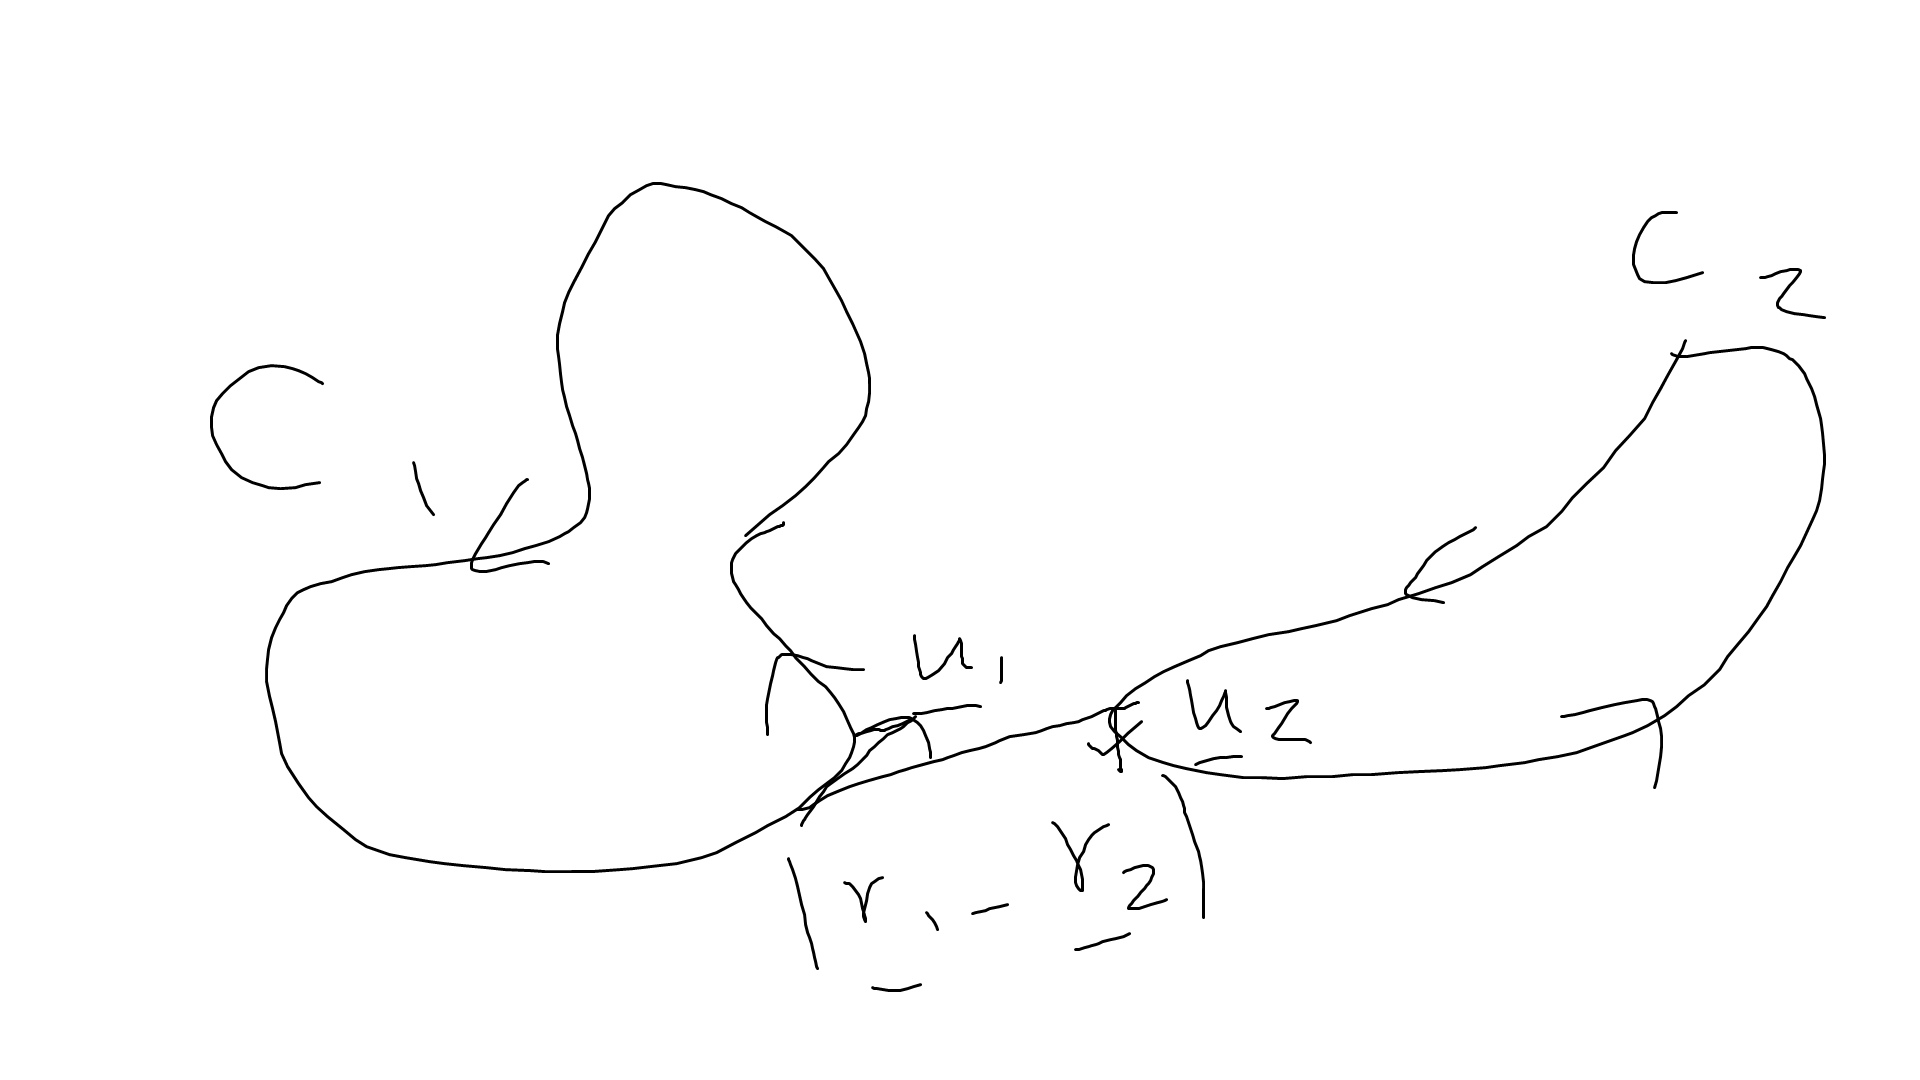
\includegraphics[scale=0.4]{EM_28}

First loop on curve $C_1$ with current $I_1$, and line element $d\mathbf{r}_1$ induces:
\begin{equation*}
\begin{aligned}
\mathbf{B}_1 (\mathbf{r}) = \frac{\mu_0 I_1}{4\pi} \oint_{C_1} \frac{d\mathbf{r}+1 \times (\mathbf{r}-\mathbf{r}_1)}{|\mathbf{r}-\mathbf{r}_1|^3}.
\end{aligned}
\end{equation*}
Integrated force on second loop
\begin{equation*}\tag{3.27} \label{eq:3.27}
\begin{aligned}
\mathbf{F} &= \int d^3 \mathbf{r} J_2 (\mathbf{r}) \times \mathbf{B}_1(\mathbf{r})
\end{aligned}
\end{equation*}
\begin{equation*}\tag{3.28} \label{eq:3.28}
\begin{aligned}
&= I_2 \oint d\mathbf{r}_2 \times B\mathbf{B}_1(\mathbf{r})\\
&= \frac{\mu_0 I_1I_2}{4\pi} \oint_{C_1} \oint_{C_2} \frac{d\mathbf{r}_2 \times (d\mathbf{r}_1 \times (\mathbf{r}_2 - \mathbf{r}_1))}{|\mathbf{r}_2-\mathbf{r}_1|^3}
\end{aligned}
\end{equation*}
Suppose loops are well-separated ($r=|\mathbf{r}_2-\mathbf{r}_1| > R_1,R_2$). Expand to find
\begin{equation*}\tag{3.29} \label{eq:3.29}
\begin{aligned}
\mathbf{F} = \frac{\mu_0}{4\pi} \nabla \left(\frac{3(\mathbf{m}_1 \cdot \hat{\mathbf{r}})(\mathbf{m}_2\cdot \hat{\mathbf{r}}) - \mathbf{m}_1 \cdot \mathbf{m}_2}{r^3}\right)
\end{aligned}
\end{equation*}
(See D Tong's EM notes -- non-examinable).

\newpage

\section{Electrodynamics}

\subsection{Faraday's Law of Induction}
Consider the time-dependent Maxwell's equations \eqref{eq:1.14},
\begin{equation*}\tag{4.1} \label{eq:4.1}
\begin{aligned}
\nabla \times \mathbf{E} = -\frac{\partial \mathbf{B}}{\partial t}
\end{aligned}
\end{equation*}
This shows how varying magnetic fields \emph{induces} electric fields (and, in turn, currents and further magnetic fields will be created, \eqref{eq:1.12}, \eqref{eq:1.15}).

(missing 1 lecture)

Inductance (4.8) $L=\phi/I$.

Solenoid (continued)

Field through single turn $B=\mu_0 IN$ and flux is $\phi_0 = \mu_0 INA$ and total flux is
\begin{equation*}
\begin{aligned}
\phi = \phi_0 NL = \mu_0 IN^2 Al = \mu_0 IN^2\nu
\end{aligned}
\end{equation*}

So self-inductance is
\begin{equation*}\tag{4.9} \label{eq:4.9}
\begin{aligned}
L=\phi/I = \mu_0 N^2 \nu
\end{aligned}
\end{equation*}
Work must be done to create $I$ but this is reversible.

\subsubsection{Magnetostatic energy}
How much energy is stored in wire curve $C$ with current $I$? Build up from $U=0$ and use inductance $L$ to find the work done.

Change in current $\frac{dI}{dt}$ induces EMF because of flux change (4.8)
\begin{equation*}\tag{4.10} \label{eq:4.10}
\begin{aligned}
\varepsilon = -\frac{d\phi}{dt} = -L \frac{dI}{dt}
\end{aligned}
\end{equation*}
The current must do work (recall $dV/dt = P=VI$)
\begin{equation*}
\begin{aligned}
\delta W = \varepsilon I \delta t = -LI \frac{dI}{dt} \delta t
\end{aligned}
\end{equation*}
So $dW/dt = -LI dI/dt$ which integrates to
\begin{equation*}\tag{4.11} \label{eq:4.11}
\begin{aligned}
W = \frac{1}{2} LU^2 = \frac{1}{2}I\phi
\end{aligned}
\end{equation*}

\begin{eg}
Consider solenoid with $|phi=\mu_0 IN^2 \nu$, we have
\begin{equation*}
\begin{aligned}
W = \frac{1}{2}I\phi = \frac{1}{2} \mu_0 I^2 N^2 \nu = \frac{1}{2\mu_0} B^2 \nu
\end{aligned}
\end{equation*}

The energy of steady current is stored in magnetic fields:
\begin{equation*}
\begin{aligned}
U &= \frac{1}{2} I \phi = \frac{1}{2} I \int_S \mathbf{B} \cdot d\mathbf{S} = \frac{1}{2} I \int_S \nabla \times \mathbf{A} \cdot d\mathbf{S} = \frac{1}{2} \oint_C \mathbf{A} \cdot d\mathbf{r}\\
&= \frac{1}{2} \int_V d^3 \mathbf{r} \mathbf{J} \cdot \mathbf{A}\\
&= \frac{1}{2\mu_0} \int d^3 \mathbf{r} \nabla \times \mathbf{B} \cdot \mathbf{A}\\
&= \frac{1}{2\mu_0} \int d^3 \mathbf{r} [\nabla \cdot (\mathbf{B} \times \mathbf{A}) + \mathbf{B} \cdot \nabla \times \mathbf{A}]
\end{aligned}
\end{equation*}
note that we've used Stoke's theorem, Maxwell's theorem \eqref{eq:3.1} and  the identity
\begin{equation*}
\begin{aligned}
\nabla \cdot (\mathbf{A} \times \mathbf{B}) = \mathbf{A} \cdot \nabla \times \mathbf{B} - \mathbf{B} \cdot \nabla \times \mathbf{A}
\end{aligned}
\end{equation*}
\end{eg}
So the above equals
\begin{equation*}\tag{4.12} \label{eq:4.12}
\begin{aligned}
\frac{1}{2\mu_0} \int d^3 \mathbf{r} \mathbf{B} \cdot \mathbf{B}
\end{aligned}
\end{equation*}
Also applies for several curves $C_i$, currents $I_i$. Combining this with electrostatic energy \eqref{eq:2.27} we have
\begin{equation*}\tag{4.13} \label{eq:4.13}
\begin{aligned}
U = \int d^3 \mathbf{r} \left(\frac{\varepsilon_0}{2} \mathbf{E} \cdot \mathbf{E} + \frac{1}{2\mu_0} \mathbf{B} \cdot \mathbf{B}\right)
\end{aligned}
\end{equation*}

\subsection{Resistance and heat loss}
Building up (or maintaining) current $I$ also requires irreversible work because of friction or resistance. Usually there is an effective EMF $\mathcal{E}$ proportional to the speed of the charge carriers: Ohm's law is
\begin{equation*}\tag{4.14} \label{eq:4.14}
\begin{aligned}
\mathcal{E}=IR
\end{aligned}
\end{equation*}
where $R$ is the resistance of the circuit $C$.

For a wire of cross-sectional area $A$, length $l$ the \emph{resistivity} $\rho$ is
\begin{equation*}\tag{4.15} \label{eq:4.15}
\begin{aligned}
\rho = \frac{AR}{l}
\end{aligned}
\end{equation*}
while the \emph{conductivity} $\sigma$ is $\sigma = 1/\rho$. In general, Ohm's Law is 
\begin{equation*}\tag{4.16} \label{eq:4.16}
\begin{aligned}
\mathbf{J} = \sigma \mathbf{E}
\end{aligned}
\end{equation*}

\subsubsection{Energy dissipation (Joule heating)}
In the presence of resistance, work is required to maintain a current $I$. In a time $\delta t$,
\begin{equation*}\tag{4.17} \label{eq:4.17}
\begin{aligned}
\delta W = \mathcal{E} I \delta t = I^2 R \delta t \implies \frac{dW}{dt} = I^2 R
\end{aligned}
\end{equation*}
This energy is lost as friction or heating.

\subsubsection{Moving wire example}

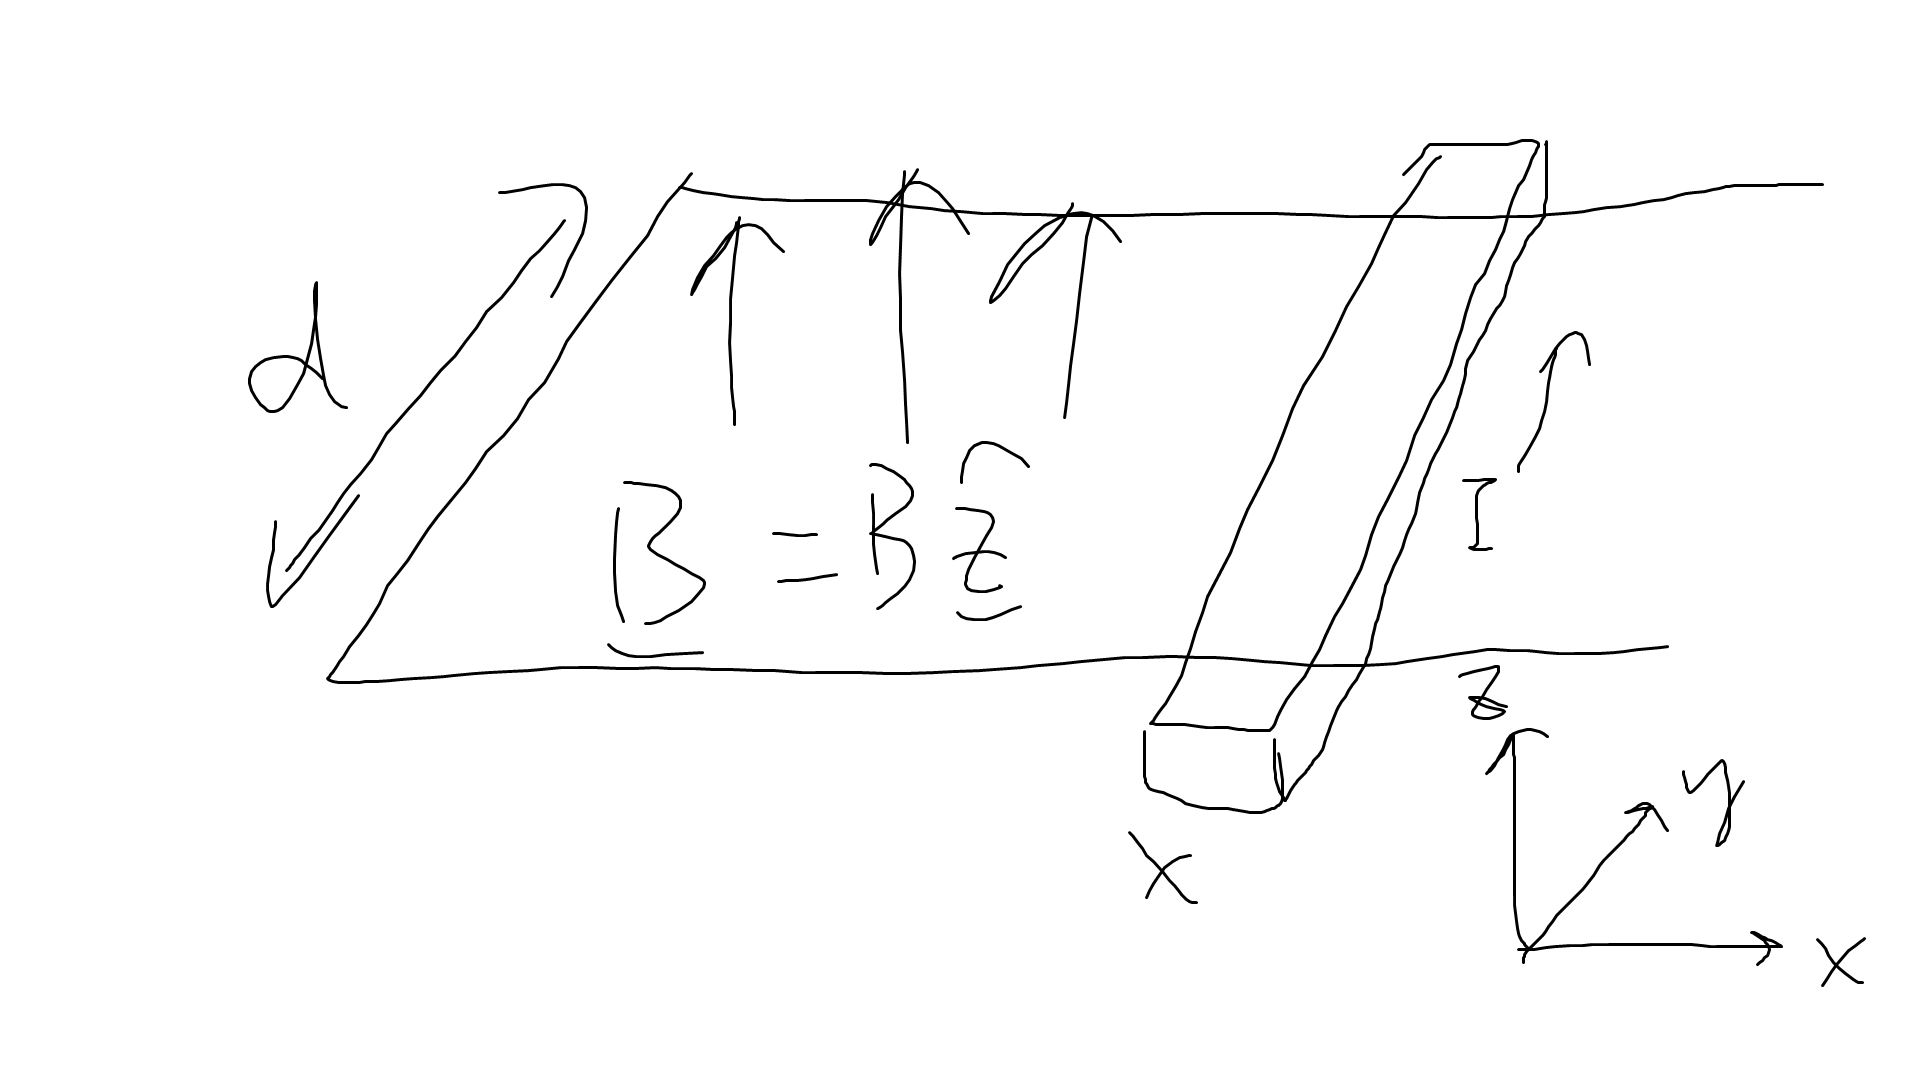
\includegraphics[scale=0.4]{EM_29}

Suppose we have a frictionless sliding bar (length $d$, mass $m$). Degrees of freedom position $x$, current $I$. For position, the Lorentz force per unit length is
\begin{equation*}
\begin{aligned}
\mathbf{f} = IB \mathbf{\hat{y}} \times \mathbf{\hat{z}}
\end{aligned}
\end{equation*}
so total force
\begin{equation*}
\begin{aligned}
\mathbf{F} = IB d\mathbf{\hat{x}}
\end{aligned}
\end{equation*}
From $\mathbf{F} = m\ddot{x}$ we have $m\ddot{x} = IBd$ (*) (we ignore $B$ due to the current itself here).

For current, we know total EMF is
\begin{equation*}
\begin{aligned}
\mathcal{E} = -\frac{d\phi}{dt} = -B dv = -B d \dot{x}
\end{aligned}
\end{equation*}
But Ohm's Law \eqref{eq:4.14} gives $I=\mathcal{E}/R = -Bd\dot{x}/R$. So we have
\begin{equation*}
\begin{aligned}
m \ddot{x} = -B^2 d^2 \dot{x}/R
\end{aligned}
\end{equation*}
which has the decaying solution
\begin{equation*}\tag{+}
\begin{aligned}
\dot{x} = -v_0 e^{-B^2d^2t/mR}
\end{aligned}
\end{equation*}
where $v_0$ is the initial velocity. Whichever way the bar moves by Lenz's law acts against the motion. Current obeys
\begin{equation*}
\begin{aligned}
I = \mathcal{E}/R = -Bd\dot{x}
\end{aligned}
\end{equation*}
so the energy dissipates 
\begin{equation*}\tag{4.17}
\begin{aligned}
dW/dt = \mathcal{E} I = I^2R.
\end{aligned}
\end{equation*}

With a battery with EMF $\mathcal{E}$ included a current $I_0 = \varepsilon_0/R$, the total EMF becomes
\begin{equation*}
\begin{aligned}
\mathcal{E} = \mathcal{E}_0 + \mathcal{E}_{induced} = \mathcal{E}_0 - Bd\dot{x}
\end{aligned}
\end{equation*}
Again using Ohm's Law $\mathcal{E} = IR$ we have
\begin{equation*}
\begin{aligned}
m \ddot{x} = IBd = -Bd/R(Bd\dot{x}-\mathcal{E}_0)
\end{aligned}
\end{equation*}
This is simple to solve exploiting the solution (+).





\end{document}